\documentclass{wustlthesis}

\setmainfont{Times New Roman}               % Use Times New Roman
\setmathfont{STIXTwoMath}[math-style=ISO]   % Use math font that matches Times New Roman

% Re-calculate the lengths of a text line using the current font
\setlxvchars[\normalfont\normalsize]
\setxlvchars[\normalfont\normalsize]
\checkandfixthelayout[classic]

%Read ai files
\usepackage{graphicx}
\DeclareGraphicsRule{.ai}{pdf}{.ai}{}
% Enable refinements of typographics
\usepackage[
    activate=true,
    %disable=false,  % enable microtype even in the draft mode
    babel=true,     % enable language-specific kerning.
]{microtype}
%\DeclareMicrotypeAlias{Times New Roman}{ptm}
% Tweak LaTeX line breaking
\midsloppy

% Hyperlinks
\usepackage{hyperref}
\hypersetup{%
    colorlinks=true,
    linkcolor=black,
    urlcolor=[rgb]{0.0855,0.3675,0.5470},
    citecolor=black%
}
% default URL style
\urlstyle{same}

% Tables (optional packages)
\usepackage{threeparttable}
%\usepackage{makecell}  % allow multiple lines in a table cell
\usepackage{multirow}   % allow multiple lines in a table cell

% for the degree
\usepackage{gensymb}
\let\dg\degree
% Graphics
\usepackage{graphicx}
%forsuppfigure
\usepackage{newfloat}
\DeclareFloatingEnvironment[
    fileext=lof,
    name=Figure,
    placement=tbhp,
    within=chapter,
]{suppfigure}
\DeclareFloatingEnvironment[name={Supplementary Table},within=chapter,placement=tbhp,fileext=lsf,listname={List of Supplementary Tables}]{supptable} % Set up supplementary figures
% Add newcommand to set up the numbering of supplementary figures and tables
\newcommand{\beginsupplement}{%
        \setcounter{table}{0}
        \renewcommand{\thetable}{S\arabic{table}}%
        \setcounter{figure}{0}
        \renewcommand{\thefigure}{S\arabic{figure}}%
}


% Subcaptions
% The caption format is "Figure 1. Some caption. (A) subcaption. (B) subcaption".
% And the label reference format is "Figure 1A".
\usepackage{subcaption}
\renewcommand\thesubfigure{\Alph{subfigure}}
\renewcommand\thesubtable{\Alph{subtable}}
\captionsetup{subrefformat=parens}

% Allowing subcaptions when all figure panels are combined
% into one source image. Based on https://tex.stackexchange.com/a/255790
\newcommand{\phantomlabel}[1]{%
    \parbox{0pt}{\phantomsubcaption\label{#1}}%
}

% Add a note for figure caption spanning multiple pages
\newcommand{\legendcontdnote}{%
    \sourceatright[2em]{%
        \footnotesize\itshape(legend continued on next page)%
}}
\newcommand{\legendcontdref}[1]{%
    \emph{(\fref{#1} continued)}%
}

% Bibliography
% use BibLaTeX + Biber and Nature citation style.
% some extra configurations:
%   - Hide ISBN and URL
%   - Display DOI
%   - Show up to 9 authors
%   - Enable back references
\usepackage[
    backend=biber,
    style=nature,
    date=year,
    isbn=false, url=false, doi=true,
    minnames=1, maxnames=9,
    backref=true
]{biblatex}
% rename bibliography section name
\DefineBibliographyStrings{english}{
    bibliography = {References},
    backrefpage = {cited on p\adddot},
    backrefpages = {cited on pp\adddot}}
% hide PubMed ID (pmid:xxx) in the bibliography
\DeclareFieldFormat{eprint:pmid}{}

% define the bibliography path
\addbibresource{references.bib}



% Configure title page
\settitle{Understanding the sources and consequences of cell-to-cell variability in gene expression}
\setauthor{Avinash Ramu}
\setthesistype{Dissertation}
\setthesisdegree{Doctor of Philosophy}
\setthesisdegreeabbrv{Ph.D.}
% Degree officially earn date must be in December, May, or August
\setdegreedatemy{May}{2023}
\setthesisadvisorwithtitle{%
    Professor Barak A Cohen, Chair}
\setthesiscommittee{%
    Barak A Cohen, Chair\\
    Tim Schedl \\
    Gary D. Stormo \\
    Shankar Mukherji \\
    Nathan O. Stitziel
}
\setthesisschool{Division of Biology and Biomedical Sciences}
\setthesisdepartment{Human and Statistical Genetics}


% Configure PDF metadata
\hypersetup{
    pdftitle={%
        Causes and consequences of cell-to-cell variability of gene expression.
    },
    pdfauthor={\thesisauthor},
}


\begin{document}

\thetitlepage                       % Title page
\frontmatter
\thesiscopyright{%                  % Thesis copyright page
    \textcopyright~\degreeearnyear, Avinash Ramu}

\SingleSpacing*
\setSingleSpace{1.15}
\tableofcontents*                   % Table of contents (ToC)
\listoffigures                      % List of figures (LoF)
\listoftables                       % List of tables (LoT)

\DoubleSpacing
\thesisacknowledgments

First, I would like to thank my thesis mentor Barak Cohen. I was in a tough spot when I joined Barak's lab, a sinking ship I think Barak called it. The PI of the lab I had joined decided to move out of WashU towards the end of the second year of my PhD. I'm extremely thankful that Barak gave me an opportunity to join and train in his lab. Barak's mentoring is something I will really miss to say the very least. He put my development as a scientist at the forefront of my PhD, and was able to help me identify my strengths and weaknesses right at the start of my PhD (starting at the rotation.) He encouraged all of us to attend seminars, department events and always set an example by doing things himself first. He gave me complete independence as a computational student doing experiments to seek out external core/industry services that would make my experimental load lighter. He gave me complete freedom in my work, trusted me to make the right decisions and encouraged me to be fearless. The work in Chapter 3 just started as a conversation amongst three graduate students and Barak was supported and encouraged our ideas from the beginning. I could tell right from the beginning that the years I spent in Barak's lab were going to be some of the most formative years of my life.

Next, I would like to thank my wife Alicia for her kindness, constant fun presence and thoughtfulness from before and throughout graduate school. We got married and welcomed our son Arjun during graduate school. There were innumerable occasions of me complaining to her about something that didn't work and she helped me see my blind spots and the bigger picture on many such occasions. Her work in Global Health also helped me realize the massive present day challenges facing the world and helped me put my work in perspective. Thank you for being there, I truly couldn't have finished this thesis without you and I feel lucky to have you in my life. Thanks also for introducing me to your amazing parents, Karen and Juan, your family and many of your friends who later became my friends. They were all vested in my success during this program.

I would like to thank my Mom for always checking in on me during graduate school and for coming over to watch Arjun during the chaotic few months after his birth. I'd also like to thank my sister for watching over my mom in India. I'm grateful for the opportunity to live away from where I grew up and pursue this career, something that would have not been possible for me without the efforts of my parents.

I would like to thank my thesis commmittee members - Tim Schedl, Gary Stormo, Shankar Mukherji and Nate Stitziel. Every one of them met with me outside committee meetings and I took it upon myself to learn from their varied expertise. I'd especially like to thank my chair Tim Schedl. Tim helped me on numerous occasions through graduate school. He helped me figure out a lab when I had to find a new lab towards the end of my second year. There were innumerable occasions that I would just stop by Tim's office to chat about something interesting that I'd read or heard just to have a conversation and see what he thought about it. I found these conversations an amazing learning experience and also fun to just chat with him. I will miss these conversations. He was always welcoming and I feel really fortunate that I could receive his mentorship throughout graduate school. The Precision Medicine Pathway that Tim organized offered me innumerable occasions to interact with and learn from top researchers from around the world. Thank you Tim.

I'd also like to thank all the HSG faculty and the program directors John Rice and Nate Stitziel, and the previous director Pat for making the program such a friendly place to learn and do research. I'd like to especially thank Nancy Saccone for answering all my questions related to statistical genetics, hosting journal club and for helping work on a project related to Polygenic Risk Scores. I'd like to also thank my mentors prior to graduate school, Malachi Griffith and Obi Griffith for their support and mentorship when I worked in their lab. They were incredibly supportive of my decision to apply to graduate school while working in their lab. I'd like to also thank Don Conrad for sharing his insatiable passion for human genetics with me during the years I spent in his lab.

I would like to thank my lab mates for a fantastic intellectual atmosphere to do a PhD in and asking me the tough questions during lab meetings. I'll definitely miss our lab meeting environment. I'd like to especially acknowledge Siqi and Clarice, whom I worked closely with on the work described in Chapter 3. Attending both their weddings was one of the biggest highlights of my graduate school life. Siqi also helped me get started on experiments in the Cohen Lab and I owe a lot to him for transitioning from being completely lost to just occasionally lost. I'd also like to thank Dana King who was incredibly supportive when I first joined the lab. I always enjoyed chatting with Dustin Baldridge about human genetics research, sharing the same experimental 3T3 system with Dustin gave me some company in my solitary efforts. Also, thanks to everyone on the fourth floor of the Couch building for the many conversations over coffee/tea and lunch. I'll miss just sitting outside in the lobby area with a cup of tea and laptop in front of me.

WashU has been an incredible place for me to pursue my PhD, and I am deeply grateful for this opportunity. I joined WashU as a staff Bioinformaticist in August 2011, and my experiences here made me interested in applying to graduate school. My awe for the university grew with every passing year as I began to understand the incredible work that was being done here over such a long time. Walking through the halls where many scientific legends had walked and the pivotal human genome had been sequenced was not just intimidating but also inspiring. I would like to acknowledge DBBS for a fantastic training environment for my PhD. The program is so flexible in it's present form and let me pursue any research area that I was interested in. I'd especially like to acknowledge Sara Holmes for help behind the scenes with my PhD and all my fellow DBBS students I worked with at the Student Advisory Committee (SAC). Doing a PhD definitely took a toll on my physical and mental health but thanks to the fantastic health resources available to DBBS PhD students at Student Health this was manageable for me. 

I would like to personally thank Abul Usmani whom I know from my time in Don Conrad's lab for sharing his experimental knowledge with me and showing me around the wet-lab. Thanks also to Xuhua Chen from Rob Mitra's lab for sharing her wet-lab genius with me, the project in Chapter 2 and Chapter 3 would not be possible without her guidance with the 10X protocol. Chatting with Xuhua often helped me forget my wet-lab worries. Thanks to Jess, ML, Brian and Eric for enabling the CGS be a fantastic place to do genomics research.

I would like to acknowledge all my friends both in St. Louis and beyond - Harry, Jia, Ching, Kuan, Kalpit, Deepak, Niel. Thank you for directly or indirectly supporting me throughout this journey with your great company, often over boardgames, dinner, movies or cricket.

The work of Jon Kabat-Zinn \cite{ludwig2008j} helped me try to stay present, especially during stressful times and made me think deeply about the bigger picture of life. I'm  thankful that Jon switched to the work he does after starting out as a molecular biology scientist.

Finally, thanks to Sky and Arjun for sharing your playtime with me and reminding me of the joys of life everyday.

\null\hfill \thesisauthor

\noindent
\textit{Washington University in St.\@ Louis}\\
\textit{May 2023}
    % Acknowledgements
\thesisdedication{%                 % Dedication page
    To Alicia, Sky and Arjun.
}
\begin{abstract}

Gene expression is a stochastic process. A population of genetically identical cells grown in an identical environment can express different amounts of any given gene. This cell-to-cell variability in gene expression often underlies important phenotypic differences between cells. If we can understand the sources of cell-to-cell variability in gene expression this will further our understanding of the mechanisms of transcription. The core of this thesis is split into two chapters. One chapter I examine the impact of cell-to-cell variability on a specific phenotype, a signaling pathway response. In another chapter I discuss the results of using a novel technology that I developed to uncover the sources of cell-to-cell variability.

In the second chapter, I examine cell-to-cell variability in a signaling pathway response. The hedgehog signaling pathway is an important developmental pathway. We examine cell-to-cell variability in how fast genetically identical cells can respond to stimulation of this pathway using a well established cell-culture model of hedgehog signaling. We identify two groups of cells, one that can respond very fast to hedgehog stimulation and another that responds on a slower timescale. We hypothesized that stochastic  fluctuations in transcription factor activity could underlie functional differences between these subsets of cells. Using computational analysis of single-cell RNA sequencing data I identified multiple transcription factors that are differentially expressed between the fast responders and the slow responders. Overexpression of four of these transcription factors is sufficient to create the fast responder cell-state. I also found that overexpression of one of the transcription factors, \emph{Prrx1} is also sufficient to drive the fast response. We conclude that stochastic cell-to-cell variability of \emph{Prrx1} underlies part of the cell-to-cell variability in how fast a given cell responds to hedgehog pathway stimulation. An important follow-up question that I tackle in the next chapter is what are the factors that determine the cell-to-cell variability of different genes in the genome.

In the third chapter I helped develop a novel technique for measuring  the factors underlying cell-to-cell variability. Specifically, I looked at the effect of genomic environments and cellular environments on cell-to-cell variability. The method is called Single-cell Analysis of Reporter Gene Expression Noise and Transcriptome (SARGENT). Using this method we integrate the same reporter in multiple genomic locations and measuring the expression of the reporter gene at a single-cell level. This helps us estimate the expression mean and variance of the reporter gene at multiple genomic locations. Using SARGENT we also measure the global transcriptome of the same cells expressing the reporter. We then associated the cell-to-cell variability of the reporter at different genomic locations with the chromatin marks at the different genomic locations. We find that the chromatin marks that are associated with the cell-to-cell variability are often different from or have a different direction of association compared to the chromatin marks that are associated with the mean level of expression. We used the global transcriptome to understand the effect of cell state on the cell-to-cell variability. Finally, using pairs of reporters observed in different cells we decomposed the total cell-to-cell variability into extrinsic and intrinsic noise and find that the cell-state has an effect on the extrinsic noise. 

Cell-to-cell variability in gene expression, amongst genetically identical cells in the same environment can have functional consequences. One such consequence that I detected is the variability in the timing of response to hedgehog stimulation. The sources of cell-to-cell variability are important to understand both to further our fundamental understanding of the mechanisms of transcription and for practical reasons such as genome engineering and gene-therapy efforts. The genomic and cellular environment features associated with cell-to-cell variability uncovered in this thesis are good candidates for further examination of the sources of noise.

\end{abstract}

\mainmatter
\pagestyle{main}

\chapter{Introduction}
\label{chap:introduction}
\tightlists

As a geneticist, my main goal is to shed more light on how genotype results in phenotype. These can be phenotypes at any level, for example at the cellular level, tissue level or organismic level. We know that DNA sets the blueprint for all the phenotypes of an organism. The first and arguably one of the most important steps in the process of going from DNA to cellular machines is gene expression. DNA gets transcribed to RNA and these are then translated to proteins, and these are the molecules that set up life as we know it - both inside us and around ourself. We function as who we are due to the concerted action of these DNA, proteins and RNA.

So, to understand how genotype translates to phenotypes it is key to understand gene expression. There are indeed a large number of research programs devoted to understanding gene expression. This thesis also attempts to answer a question related to gene expression. Specifically, how is gene expression regulated amongst a population of cells?

Let's peek inside a single-cell. In most cell-types in a human body there are two copies of each chromosome. A small part, about 1\% of this DNA is what codes for proteins \cite {lander2001n}. Through a series of molecular steps that we don't quite yet understand, genes are turned on and off in a precise manner during development. It is this precise turning on and off of genes that generates a whole organism from a single-cell and the multitude of cell-types and organisms inside and around us. When we hear of such precision, one might think of a well oiled machine that is entirely predictable. A machine that turns on and off in an entirely predictable manner within a cell. But this is not what we observe.

We have become really good at measuring gene expression both in a population of cells \cite{bulk rnaseq, }, and now within a single-cell \cite{macosko2015c, flow cyto, xia2019pnasu, raj2006pb}. If it were true that the gene expression operates in a predictable manner, if we start with a single cell and follow gene expression in it's daughter cells, the cells would express identical amounts of RNA and protein. However this is not what one observes \cite{elowitz_stochastic_2002}. There is a tremendous amount of cell-to-cell variability in gene expression amongst a population of cells. This thesis deals with understanding this cell-to-cell variability - how does this cell-to-cell variability come about i.e its sources, and does this variability have any phenotypic impact i.e its consequences. In this thesis, I use cell-to-cell variability in gene expression and gene expression noise interchangeably.

\section{Gene expression variability exists amongst cells}

Gene expression is the result of probabilistic interactions between molecules in the cell. These molecules include the two copies of DNA, transcription factors, RNA polymerase amongst others. The low numbers of molecules involved in transcription can results in  variable gene expression across cells and time. It is still a mystery how even in the presence of these fluctuations  biological systems function in a reliable manner.

The phenomenon of variability between cells is not new. Novick and Weiner \cite{novick_enzyme_1957} \cite{raj_nature_2008} described a phenonmenon in 1957 where given a population of E. Coli, the fraction of cells that produce beta galactidase is not deterministic at low inducer concentrations. This fraction varies with the concentration of the inducer. The increase in the concentration of inducer only increases the chance that a bacterium produces beta galactidase. Given a fixed concentration of the inducer, it is not possible to predict with certainty if a single bacterium will produce beta galactidase but it is possible to estimate the probability of this event. This is fascinating. This paper is also one of the earliest works that I am familiar with that talks about variable cell-state - there's an induced state and a non-induced state and the whole question is about the transition from one cell-state to another. The authors also compare the enzyme induction state to a mutation.

Now let us turn to variability in gene expression. In 2002, Elowitz et al.  \cite{elowitz_stochastic_2002} showed using two-colored reporter genes in E. Coli that identical genes on two different chromosomes show cell-to-cell variability in expression. The authors decomposed this variability into two components. The first is intrinsic noise that is specific to a locus. Intrinsic noise is due to the local interactions of molecules involved in transcription at a locus. These might include promoters switching between active and inactive states, proteins binding to enhancers, recruitment of RNA polymerase and so on. The second source of variability is extrinsic noise. Extrinsic noise is due to differences between cells in what is commonly termed the cellular milieu. The cellular milieu can include upstream regulators of transcription such as transcription factor concentrations, number of ribosomes in the cell, differences in cell cycle stage, differences in mitochondrial number etc. These differences in the cellular environment is likely to affect the expression of multiple genes. Several other studies that came out around roughly the same confirmed the observation that genetically identical cells in the same environment display variability in gene expression, this phenomenon is observed in cells from multiple organisms. \cite{raser_control_2004,blake_phenotypic_2006,blake_noise_2003,raser_noise_2005,volfson_origins_2006}.

Following these studies variability in gene expression has also been observed and modeled at the RNA level. As an example of an early study, in 2006 Raj et al \cite{raj2006pb} counted the number of mRNA molecules of using fluorescence in situ hybridization (FISH). They found a large variation in the number of mRNA molecules between cells of the same cell type. They find that most of the variability they measure is due to intrinsci noise. They then modeled the mRNA distributions using a stochastic model of gene transcription and show transitions between an inactive state and a state of active transcription can result in such cell-to-cell variability. They observe variations in burst size, which they attribute to transcriptional activators, but they did not find that the data fit changes to burst frequency. This work marked the beginning of a series of studies that used the cell-to-cell variability in the mRNA molecules to understand mechanisms of transcription \cite{symmons2016mc} \cite{Chen and Teichmann and Meyer 2018 from Larson paper}.

More recently it has become possible to visualize transcription in live cells and infer mechanisms of transcription. For example, in 2019 Rodriguez et al. \cite{rodriguez_intrinsic_2019} used live-cell RNA imaging to look at the regulation of hte estrogen-responsive gene TFF1. The authors observe periods where the gene is transcriptionally active or inactive. The inactive periods vary hugely, they can range from periods in minutes to many hours. The active periods are much  shorter and are of the order of 16 minutes on average. They also find instances of allelic coupling where transcription of one allele influences the transcription of the other allele more likely. Deletion of an enhancer region increases the inactive time period, which fits with the literature reflecting that enhancers control burst frequency. Using single-cell RNA sequencing data, the authors postulate that the deep repressive state that is observed for TFF1 could extend to other genes in certain functional categories such as secretion, transmembrane and signal peptides. Their modeling reveals a deep repressive state  which a gene could spend hours in a repressive state. It remains to be seen if this deep repressive state is observed in cells in the future, this paper used observation times of 14 hours which is insufficient to observe this state. If this state is real it would be fascinating to understand the mechanisms at the DNA level that underlie this state again revealing the fascinating ways in which cell-to-cell variability can unveil mechanisms of gene expression.

As time passed, technical innovations have helped us peer at different molecules within cells and they have all revealed that cell-to-cell variability in gene expression is ubiquitous. But does this cell-to-cell variability matter?

\section{Cell-to-Cell variability can result in functional differences}

An increase in cell-to-cell variability in gene expression has been observed in cells undergoing differentiation. Richard et al.  \cite{richard_single-cell-based_2016} looked at a well-studied differentiation system of chicken erythroid progenitors differentiating into erythrocytes. The authors showed that chicken erythroid cells show an increase in variability of gene expression of relevant genes prior to differentiation. Similar results were obtained by Mojtahedi et al  \cite{mojtahedi_cell_2016} while studying the differentiation of murine heamatopoetic progenitor cells into myeloid or erythroid cells. The authors hypothesize that this surge in variability allows the cells to transition out of stable cell-states and transition to different cell-states. 

Other examples have shown that genetically identical cells don't all reprogram at the same rate. Hanna and Saha et al. showed that reprogramming of somatic cells to iPSCs is stochastic with a random subset of initial cells completing reprogramming  \cite{hanna_direct_2009}. The authors showed that eventually all somatic cells reprogram to pluripotent stem cells when induced with transcription factors but the rate at which cells reprogram can be increased by increasing the cell-division rate. Similar stochasticity has been observed when fibroblasts were reprogrammed into induced endoderm progenitor cells \cite{biddy_single-cell_2018}.

Variability in phenotype has also been shown to be functionally important at the organismal level. In C. elegans, two identical cells from different lineages known as alpha cells always give rise to exactly one ventral uterine progenitor cell and one anchor cell \cite{seydoux_cell_1989}. Both the alpha cells have the potential to generate either of the two downstream cell-types but the cell fate is decided in a stochastic and co-ordinated manner. This case is a well-studied model of a stochastic cell-fate decision where a robust outcome is produced as a result of a stochastic choice. In another example in C. elegans, mutations that cause incomplete penetrance have been shown to be due to increased variability in the expression of cell-fate determining genes  \cite{raj_variability_2010}.  The mutants display increased variability in the expression of a gene called *end-1*. Cells with high-levels of *end-1* are able to activate downstream targets in the intestinal fate specification network whereas the cells with low levels of *end-1* do not. 

In bacteria, individual bacterium often display a persistor phenotype and grow at slower rates by expressing different subsets of genes. This confers the bacteria an ability to survive adverse changes such as antibiotic treatment that might otherwise terminate a homogenous population \cite{veening_bet-hedging_2008}. In yeast, variability has been observed in the utilization of the sugar galactose. The Gal genes that are responsible for the metabolism of galactose pathway display a bimodal expression pattern \cite{acar_enhancement_2005}. This bimodality has been explained using stochastic modelling of the expression of genes in this pathway. These results all show how biological variability, arising from variability in gene expression, can have functional consequences. 


\section{RNA sequencing can be used to uncover cell-to-cell variability}

RNA sequencing, both at the bulk and single-cell level, can be used as a readout of functional cell-states. A prominent example is the work by Chang et al. \cite{chang_transcriptome-wide_2008}. Chang et al. isolated mouse heamatopoetic progenitors with different levels of a haematopoetic stem-cell marker Sca-1.  Sca1 expression showed reproducible variability across cells that was not just due to technical error in measurement. The authors used microarrays to show that cells with low amounts of Sca-1 had different transcriptomes compared to cells with low amounts of Sca-1. Furthermore, cells with higher levels of Sca-1 have an increased likelihood of differentiation towards the Myeloid lineage while cells with low amounts of Sca-1 are more prone to differentiate towards the Erythroid lineage. Similar examples have been observed for embryonic mouse cells with different amounts of a stem-cell marker Nanog \cite{kalmar_regulated_2009}. The authors showed that cells with low levels of Nanog exhibit increased variability in gene expression and are prone to differentiate.

Computational modeling approaches are important to understand expression differences between single-cells. The single-cell RNA seq data gives us a static snapshot of a dynamic process. Every cell on a PCA plot is a summary of an enormous number of events. These cells are transitioning through different cell-types in a differentiating system or through different cell-states within a homogenous cell-type population. A commonly used approach to understand this dynamical process is to cluster cells with similar transcriptomes together. The predicted paths of cellular trajectories are inferred by drawing a principal curve through the cells. By correlating the expression patterns along the trajectory with known biology we can infer the processes active in these cells. \cite{trapnell_dynamics_2014}. Another recently developed method called RNA-velocity allows us to infer the near-term future transcriptome of cells. This is done by fitting a kinetic model to the ratio of spliced to unspliced transcripts of each gene. This allows the number of inferred transcript counts of different genes to be estimated. The inferred transcriptome is then plotted on a PCA or tSNE plot to infer the position where a given cell's transcriptome is headed.  \cite{manno_rna_2018} Cell state transitions can be modeled as Markov processes \cite{stumpf_stem_2017} and the RNA-velocity approach can be used to infer transition rates of the model. Using such computational models can help answer interesting questions. For example, we can try to understand the proportion of time cells spend in a certain cell-state and transition to different cell-states, how many cell-states explain the observed data  \cite{chang_transcriptome-wide_2008}, what are the characteristic markers of different cell-states, and what are the genes are driving cell-state transitions \cite{furchtgott_discovering_2017}.

A recent study used single-cell RNA-seqeuencing to estimate the burst frequency and burst size of about 7000 genes genome-wide \cite{rodriguez_intrinsic_2019}. This study used Smart-seq2 technology which provides coverage across the transcript and shows a reduced 3' bias compared to alternative technologies such as 10X. \cite{picelli2013nm} The authors estimated the average waiting time for a transcriptional burst of a gene is 4 hours though a smaller fraction of genes had waiting times of greater than 20 hours for a burst. Smaller genes have higher burst size, and the authors suggest this is expected for housekeeping genes which are usually compact and consistently expressed in most tissues. Genes with TATA elements also have a higher burst size. By applying their method to a different cell types the authors show that many DE genes show a difference in burst frequency between cell-types. The difference in burst frequency also correlates with histone marks that mark enhancer activity. The authors conclude that core promoter elements play a major role in determining burst size and enhancer elements determine burst frequencies and that cell-type specific gene expression is determined by changes in burst frequencies. This sort of genome-wide study of transcriptional kinetics can be enabled by single-cell RNA sequencing and provide a supplement to more focused, less noisy assays looking at transcription of a single reporter gene. As the capture technology for scRNA-seq improves we will get better estimates of genome-wide transcriptional kinetics and how they change across different dimensions, for example with genetic background or with age or with disease.


\section{ Noise can  be biological or technical }

\section{Genetic control of noise}

%figure1
\begin{figure}[t!]  
    \centering
    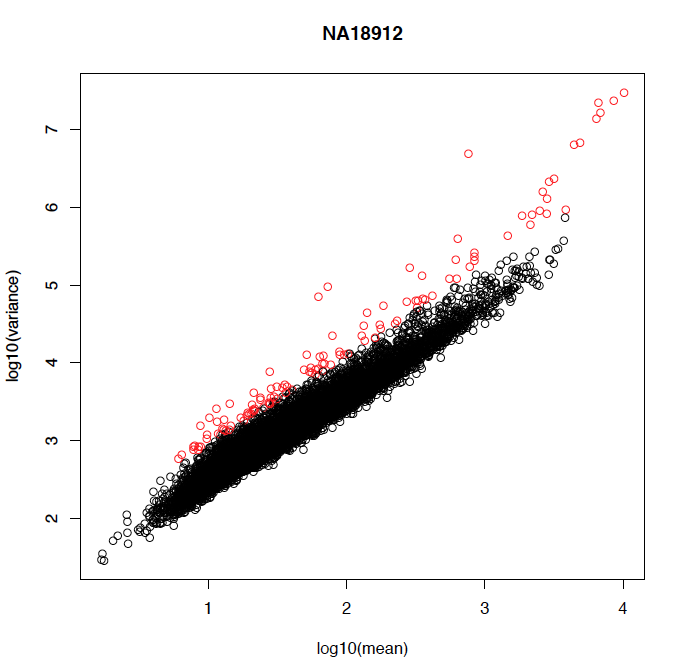
\includegraphics[width=\linewidth, scale=0.25]{figures/intro/intro_outlier1.png}
    \caption[Distribution of a Transcription Factor across cells.]{%
        \textbf{Distribution of a Transcription Factor across cells}
        The protein levels of any given transcription factor is a distribution across cells. Some cells have high amounts of the protein, some have intermediate levels, and some cells have lower amounts of the protein.
    }
    \label{fig:intro1}
\end{figure}

An important question that still remains to be answered is are the mean and noise controlled by different genetic regulatory elements.
We have made a lot of progress in identifying loci that are associated with the mean level of expression \cite{gtex_consortium_genetic_2017} \cite{vosa2021ng} \cite{more}. These studies have identified eQTLs for almost every gene in the genome and about half of all GWAS hits can now be mapped to eQTLs \cite{gtex_consortium_genetic_2017}. However this only looks at the mean level of expression. Could a similar approach be used to find loci that find variance QTLs?

Studies have looked explicitly for variance QTLs. Sarkar et al. tried to find variance QTLs using the well characterized YRI cell lines(n = 53) from the HapMap project \cite{gibbs2003n}. Briefly, they collected single-cell RNA-sequencing data from N individuals using 10X. Then they fit a negative binomial to each gene and came up with a noise measure for each gene. Since they also had genotype information for each of these individuals they looked for variance QTLs. What di they find? They found all variance QTLs were also mean QTLs. THey concluded that their sample size was too small and that they would need around 4000 number of samples to find the strongest mean independent variance QTLs at 80\% power. This study provided some methodological innovations despite being a negative result. There has been one other study that has used a simlar approach to find variance QTLs. Francesca et al. used 10X scRNA-seq data from X sampels and attempted to find QTLs. They found...

Prior to the publication of the study by Sarkar et al. I also looked at the single-cell data from their group through a collaboration with their group. I looked at cell-to-cell variability using different approaches. My variance QTL analysis also detected variance QTLs that were explained entirely by mean QTLs. I also looked at every gene's expression for every individual, and tried to find genes whose variance in gene expression was disproportionate to their mean levels. I found a set of genes that had variance above expectation consistently in many individuals (shown in red in \fref{fig:intro1}). Upon closer inspection, many of the genes that displayed this property were enriched for Mitochondrial genes. We hypothesized that mitochondrial genes might have increased variability for some functional reason. However, it is a known observation in single-cell RNA sequencing that cells that are unhealthy or dying exhibit higher levels of mitochondrial transcripts \cite {stuart2019c}, hence we did not follow up on this observation. We also used this data to look pathway specific gnees that displayed abnormal levels of variability. However, I did not find any pathways that displayed this property. Like Sarkar et al. I attribute this partly to higher technical noise of single-cell RNA sequencing as well as lower power to detect real effects due to the relatively small sample size.

\section{Selection on noise levels}

A long-standing question is whether the cell-to-cell variability of different genes are under natural selection, or does selection act only at the mean level. The alternate hypothesis is that the noise is just unconstrained by selection and all the selection acts on the mean level of expression. As discussed in the previous section, we are now beginning to identify regulatory elements that are associated with noise but not mean levels. If these regulatory elements are under selection, or if they are conserved across species, these could indicate a possible important functional role for noise that's independent of the mean level of expression of that gene. Some studies have explored this question.

Newman et al. \cite{newman2006na} measured the noise level for 2500 genes in the the yeast genome under rich and minimal media conditions. They did this by GFP-tagging each gene and measuring the fluorescence level on a cytometer. This collection of GFP-tagged yeast strains has been an invaluable resource, and indeed I used a couple of strains from this project for my early exploratory noise projects that I described in this chapter. Newman et al. found that proteins that respond to environmental cues are more noisy than other groups of genes like housekeeping genes. Zhang et al. \cite{zhang2009msb} confirm this observation for plasma transporter genes and use mathematical models to argue that higher noise promotes evolvability of favourable gene expression levels, and could be under positive selection. 

Fraser et al. \cite{fraser2004pb} looked at noise in two classes of genes in yeast - essential genes, and genes involved in protein complex subunits and compared the noise levels in these two groups to the rest of the genes in the genome. They estimated protein production rates, and transcription rates for every gene in the genome and found that the essential genes and the genes that are part of protein complexes display a lower rate of translation, and a high rate of transcription and decay - a strategy that minimizes noise. The authors speculate that this strategy might have been an evolutionary mechanism to minimize noise in genes that are essential to life.

Batada et al. \cite{batada2007ng} asked whether genes that are essential are in regions are in regions of the genome that have low nucleosome occupancy, and whether noise-sensitive genes cluster with essential genes in the genome. They reason that genes that are essential might have evolved to be in regions of the genome that are less noisy. Using Myc-tagged histone data they indeed find an anti-corrrelation between regions of high essential gene density and nucleosome occupancy. They find a dearth of essential genes in subtelomeric regions which are high noise regions of the yeast genome.

Metzger et al. \cite{metzger2015n} have looked at the promoter of a yeast enzyme that is involved in glucose metabolism in multiple yeast species. They looked at both polymorphisms that have fixed after undergoing selection through time and new mutations, induced through mutagenesis, which have not yet undergone seleection. They find that the polymorphisms have a slightly smaller effect size on the noise level compared to new mutations, suggesting the action of selection in removing some of the noise affecting polymorphisms in the TDH3 promoter. Naturally occuring haplotypes show lower amounts noise than what would be expected under neutral evolution.

The studies cited in this section have looked for signatures of selection acting specifically on the noise level. However for some of these studies it has been hard to attribute this signal entirely to the variability, and not to the mean level of expression. Indeed, most of these studies don't rule out alternative explanations for the signals of selection that are observed in the discussion sections.

\section{Noise in transcription factors}

%figure1
\begin{figure}[t!]  
    \centering
    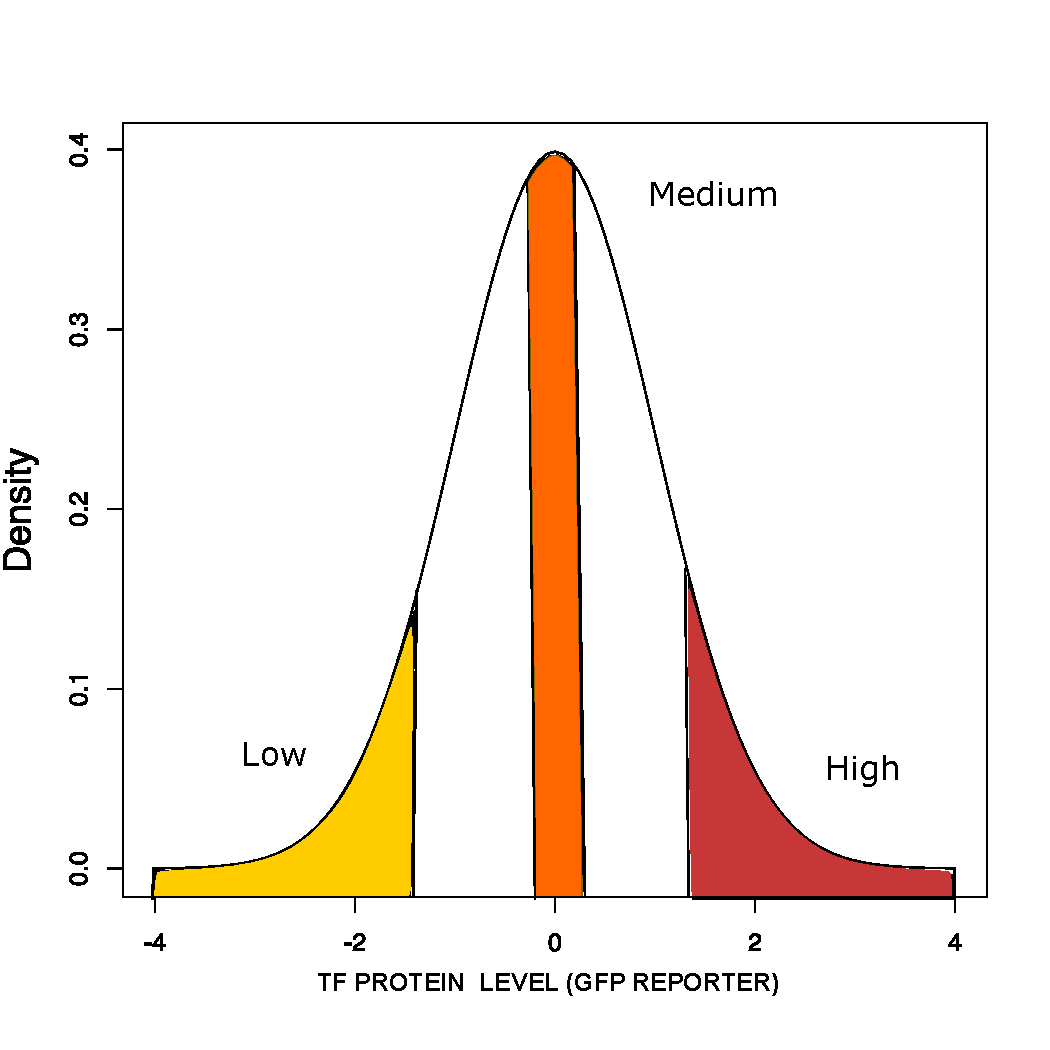
\includegraphics[width=\linewidth, scale=0.25]{figures/intro/intro_gfp_density_X.pdf}
    \caption[Distribution of Transcription Factor across cells.]{%
        \textbf{Distribution of Transcription Factor across cells}
        caption goes here
    }
    \label{fig:intro2}
\end{figure}

Consider the distribution in expression of a single transcription factor protein as shown in figure \fref{fig:intro2}. Transcription factors play vital roles in development and disease, and can convert between cell-types. \cite {Tim Hughes}. Could it then be that a cell that expresses high amounts of a transcription factor behave differently from another cell with an identical genome and growing in essentially identical environment but expressing lower amounts of the same transcription factor? Indeed, several studies have shown this to be the case across different organisms.

Wernet et al. \cite{wernet_stochastic_2006} examined the cell-fate choice in the Drosophila photorecptor cells. The drosophila eye consists of optical units called ommatidia which choose between two subtypes pale and yellow which is determined by the pairs of rhodopsin genes expressed in them. How this fate is chosen amongst genetically identical cells had been a fascinating question. The authors of this paper showed that the expression of a single transcription factor spineless is necessary and sufficient to specify the mosaic cell-fate in the Drosophila eye. Spineless is stochastically expressed in a majority of the cells which then adopt the yellow subtype. The knockout of Spineless results in all of the ommatidia adopting the blue subtype. Overexpressing spineless results in all of the ommatidia adopting the yellow subtype. This fascinating and crucial development process is thus controlled by the stochastic expression of a single transcription factor.

In \emph{C. elegans} somatic primordium four cell have the potential to be the Anchor cell (AC) which is an important cell in the gonads. \cite{attner2019cb}. How only one of these four cells becomes the AC is determined by the the transcription factor HLH-2. The rest of the four cells become the ventral uterine precursor cells (VU) cells. The relative timing of the expression transcription factor influences cell-fate in this system. The parent that expresses HLH-2 first results in the daughter becoming the VU cell. This onset of expression is also linked to the birth order of the parent cells, the parent cell that is born first also expresses HLH-2 first and adopts the VU fate. However when the birth order difference is  relatively short, the AC/VU decision appears to be random. This system is different from the previous study since it is stochastic while also being deterministic in that there is always only one AC cell, and this is determined by the birth order of the ancestor cells. The authors speculate that other stochastic outcomes might be resolved by finding other such deterministic elements. 

In Bacteria, Maamar et al. \cite{maamar2007s} examined the emergence of the transient state of competence that enables a bacterium to uptake DNA from the environment. They showed that the noise in comK the master regulator of the competence pathway involving autorogelation. This autoregulation results in bistability where in one state comK expression is low, and in the other state the comK expression is higher than a critical threshold and enables the bacterium to become competent. They show that the noise in comK is mostly intrinsic.

In this section we have seen several examples across species how the cell-to-cell variability of a single transcription factor can result in important functional differences between cells. An important follow-up question that emerges from this observation is what determines the noise levels of a certain gene? While the actual regulatory mechanisms can vary a lot between genes, certain general mechanisms of transcription can be examined for their impact on noise.

\section{Sources of noise}

\subsection{Effect of genomic features and chromatin on noise}

Several studies have looked at the effect of genomic location by integrating the same reporter gene in multiple locations. These sutudies used sequencing, time-lapse microscopy and flow cytometry approaches to look at bulk RNA and single-cell protein levels in cells. Our approach in Chapter 3 uses a similar integration strategy to look at RNA levels in single-cells to uncover the effects of cellular and genomic environment on gene expression noise.

Akhtar et al. \cite{akhtarw_vansteenselb:ChromatinPosition2013} integrated the same reporter gene in roughly 30000 locations along the mouse genome in ES cells by devising a barcode based technology called Thousands of Reporters in Parallel (TRIP). They measured the mean level of RNA expression of the reporter by using bulk RNA sequencing. The expression levels of the reporter genes vary more than 1000-fold in these locations. Nearby locations are correlated in terms of their expression and the authors used a HMM to separate the genome into permissive and non permissive domains. The non-permissive domains overlap with lamina associated domains and late-replicating domains. Permissive IR domains coincide with gene-dense and active regions. The integration locations that are promixal to genes are 10-fold more active than those located far from genes. Our technology in Chapter 3 is highly inspired by the TRIP method of Akhtar et al. The first part of our experimental pipeline is derived from the protocols of Akhtar et al. We wanted to extend TRIP to look at the factors underlying the variance of a reporter gene and not just the mean.

Dar et al. \cite{dar2012pnas} did a genome-wide study of burst frequency and burst size by using time-lapse fluorescence mircoscopy at 8,000 loci. The authors use autocorrelation time of the fluctuations as a third axis, apart from mean and noise, to understand the dynamics at different loci. The third dimension allows the authors to constrain the two-state model. They used HIV-1 lentivirus to integrate GFP driven by three different promoters. They find that bursty transcription predominates over consitutive transcription genome-wide. Both burst size and burst frequency vary in equal measure across the genome. Weaker loci modulate the burst frequency to increase expression, whereas after a certain level of expression is reached burst size is modulated to increase expression. They perturbed transcription at this loci using histone deacetylase inhibutors. They find that both burst frequency and burst size increase with increasing expression. 

Dey et al. \cite{Dey} used a lentiviral approach to integrate reporter genes at hundreds of promoters. Their approach used a dual reporter system to quantify the GFP reporter by flow-cytometry and the RNA levels by smFISH. They also assayed chromatin accessibility at the integration sites and found that higher noise locations are enriched for inaccessible chromatin. They also fit a two-state stochastic model to the data and found that the burst size determines the RNA mean while the promoter On rate influences the noise. This approach by Dey et al. provided a lot of novel insight, however multiple clones had to be measured individually as a result chromatin analysis was done on a small set of locations and the locations used in this study were not mapped. A high-throughput approach that allows for potential mapping of thousands of locations would provide more fine-grained insights.

While all three prior approaches described above furthered our understanding of how mean RNA expression and noise at the protein level changed with genomic locations, there are still some unanswered questions. Can we understand the noise at the RNA level in more locations? How does the cell-state of a cell influence the gene expression noise?

\subsection{Effect of cell state on phenotypic variability}

The previous section highlighted the effect of chromatin and genomic features of the location where a gene is situated on expression noise. A complementary factor affecting gene expression noise is the cell-state. Noise can be decomposed into intrinsic and extrinsic components \cite{swain2002pnas} \cite{raser_noise_2005}. The intrinsic component is related to the local transcriptional machinery at the gene. The extrinsic component of noise is at the cellular level and varies from cell-to-cell - for example differences in cell-cycle, cell size etc. A part of this extrinsic component can be captured by measuring the transcriptomes of individual cells \cite{macosko2015c}. This set of transcriptional measurements of each cell is also referred to as the cell-state of the cell. Recent studies have begun to examine how cell-state affects gene expression noise.

Foreman et al. \cite{foreman_mammalian_2019} measured the role of cell-state in explaining the amount of variance related to Calcium signaling after ATP stimulation. The authors also used multiplexed error robust RNA fluorescent in situ hybridization (MERFISH) to measure the cell-state of each cell by measuring the mRNA levels of 150 genes mostly related to Calcium signaling and some genes related to the cell cycle. The question that the authors were examining is how much of the variance in the Calcium signaling response can be explained by global factors such as the cell-state, cell-cycle, cell-volume and differentiation state. They also set to examine why most gene expression distributions are overdispersed. The answer is that most of the variability can be explained by cell-to-cell differences such as the cell-state and cell-size. Whatever variability remained after accounting for the cell-to-cell differences was Poissonian. This result argues that most of the noise is not gene-specific and that the shared noise dominates the allele-specific noise. This paper offers an intriguing conclusion that transcriptional bursting might not be as prevalent as previously described and that after accounting for the cell-state most genes don't follow a bursty model of transcription. While it remains to be seen how much of this finding translates to other models of study outside Calcium response, it becomes necessary to measure cell-state in any study related to gene expression noise. Our method in Chapter 3 meets this need.

Torre et al. \cite{Torre} used a genetic screening approach to find genes that regulate a drug-resistant cell-state. This drug-resistant cell-state is initially transient and rare (about 1 in 2000-3000 cells) but upon treatment, these become a stable cell-state.  The authors were interested in understanding what are the pathways that control the transient drug resistant state in the first place. This approach could potentially uncover genes that are missed in a classic drug-resistance screen. They tested two genes identified in the screen DOT1L and LATS2 which increased the frequency of the primed state and BRD2 which resulted in fewer primed cells. Along these lines, they found that the knockout of DOT1L and LATS2 results in larger tumor volumes and knockout of BRD2 results in smaller tumor volumes. This sort of genetic-screening approach can help identify the regulators of cell-states that underlie phenotypic variability. One thing that is essential to know is some sort of marker of the cell-state one is interested in. In the Torre et al. study they could sort cells based on expression of NGFR and EGFR which mark the primed cells.

Topoleweski et al. \cite{topolewski2022ssb} looked at cell-to-cell heterogeneity in the JAK-STAT signaling pathway response. The authors wanted to test if most of the variability could be explained by differences between cells in their cytoplasmic content, which would reflect cell-state or if the variability could be explained by just the local intrinsic fluctuations of genes also referred to as intrinsic noise. The authors used an interesting approach by fusing together fibroblast cells to form binuclear synctia. The reason that the fused cells could approximate as two cells with the same molecular content. The authors find that the response of two nuclei is almost always identical and explains 91\% of the variance. The remaining noise is just around 9\%. The authors speculate that the cell-state or the molecular phenotype of a cell coudl result in the cells interpreting the same signal differently. Thus the phenotypic variability doesn't argue against reliable functioning of single-cells but reflects variability in the content of cells. It still remains to be well understood how the differnt molecular phenotypes can result in variable outcomes, can we for example predict how a cell will respond to a stimulus using its transcriptome. Such approaches are likely to be possible in the future.

\subsection{ How does noise propagate within a network}

Extrinsic noise reflects global cell-to-cell differences such as cell-cycle, cell-size and affects many genes within a cell. It is still unclear what are the different levels at which extrinsic noise can act. For example can extrinsic noise act at the level of pathways?

One of the questions that I asked early in my thesis work was whether the noise in an upstream regulator of a pathway propagates within it's network. The way I tested this was by using one of the GFP-tagged yeast strain for the gene TDH2 from Newman et al.\cite{newman2006na}. TDH2 is an enzyme that plays a role in the glycolysis pathway. We hypothesized that levels of this enzyme in a given yeast might manifest as differences in the transcriptomes between yeast and possibly phenotypic differences between yeast. If the noise in TDH2 propagated downstream to the other genes in the pathway then we would be able to see differences in the target genes. 

\begin{figure}[t!]  
    \centering
    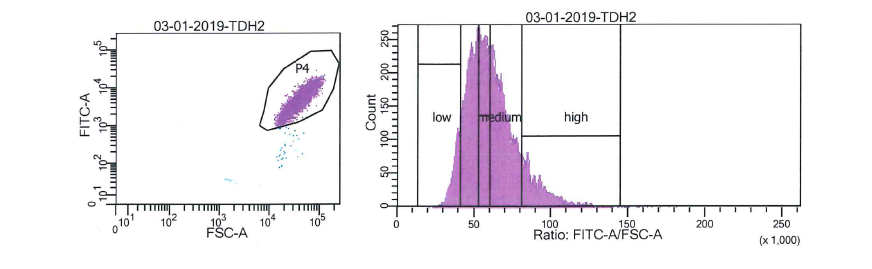
\includegraphics[width=\linewidth]{figures/intro/intro_tdh2_facs.png}
    \caption[Representative sort results of TDH2]{%
        \textbf{Representative sort results of TDH2}
        Yeast with GFP-tagged copies of the gene TDH2 were grown out and sorted on a flow sorter. Three populations of yeast with relative high, medium and low amounts of TDH2-GFP were sorted into individual tubes.
    }
    \label{fig:intro3}
\end{figure}

I sorted out three populations of cells as shown in \fref{fig:intro3}. One population expressed TDH3 at a relatively high level, marked by high levels of GFP, another population at a lower level, and another population at an intermediate level between the high and low levels.  I sorted these two populations into three separate vials, extracted RNA from the three populations and measured the transcriptomes using RNA-seq.

\begin{figure}[t!]  
    \centering
    \phantomlabel{fig:intro4a}
    \phantomlabel{fig:intro4b}
    \phantomlabel{fig:intro4c}
    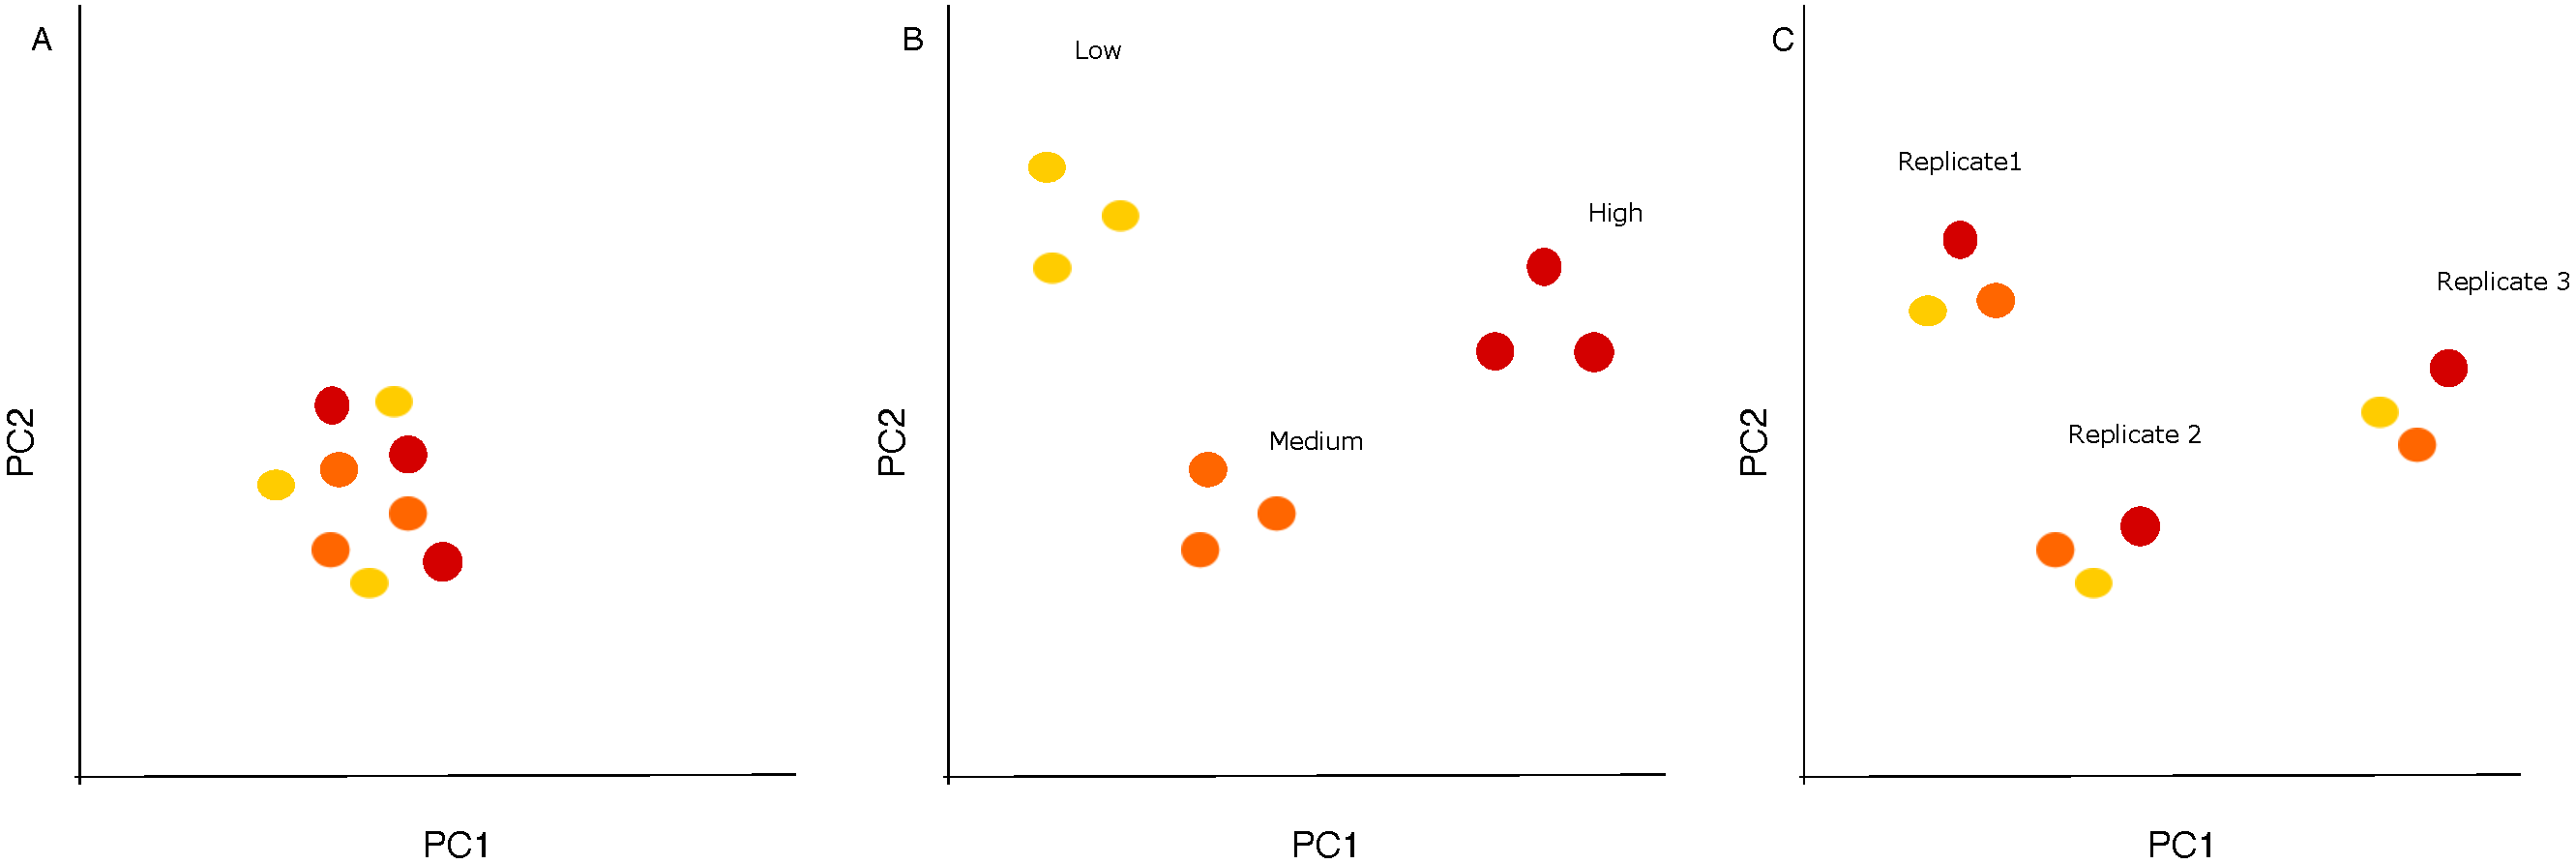
\includegraphics[width=\linewidth, scale=0.5]{figures/intro/intro_clustering_expectedresults.pdf}
    \caption[Expected results from sorting out populations with high, low and medium levels of a protein as in \fref{fig:intro2]{%
        \textbf{Expected results from sorting out populations with high, low and medium levels of a protein as in \fref{fig:intro2}}
        A) The transcriptomes don't show any discernible pattern. B) The transcriptomes separate out by the levels of the sorted protein. C) The transcriptomes separate out by a technical factor like batch.
    }
    \label{fig:intro4}
\end{figure}

What might we expect from the transcriptomes obtained from an experiment. There are three posibble outcomes if we use a clustering analysis like PCA. If the levels of the enzyme did not result in any distinct transcriptional changes, and by extension phenotypic differences amongst populations, then we would expect the transcriptomes from the high, low and medium populations to overlap as seen in Figure \fref{fig:intro4a}. If the high and low levels of the enzyme result in distinct transcriptional states, due to upregulation of the pathway in the high cells, we would expect to see the results in Figure \fref{fig:intro4b} where the high, low and medium levels of TDH2 result in distinct transcriptional states that cluster separately. This is similar to what Chang et al see in embryonic stem cells with different levels of Sca1 \cite{chang2008n}. If the experiment-to-experiment variability and batch effects of the experiment dominate the within day variability then we would expect to see the results in Figure \fref{fig:intro4c} where the samples cluster by replicate i.e the day of the experiment. This framework helps us look at the observed data.

\begin{figure}[t!]  
    \centering
    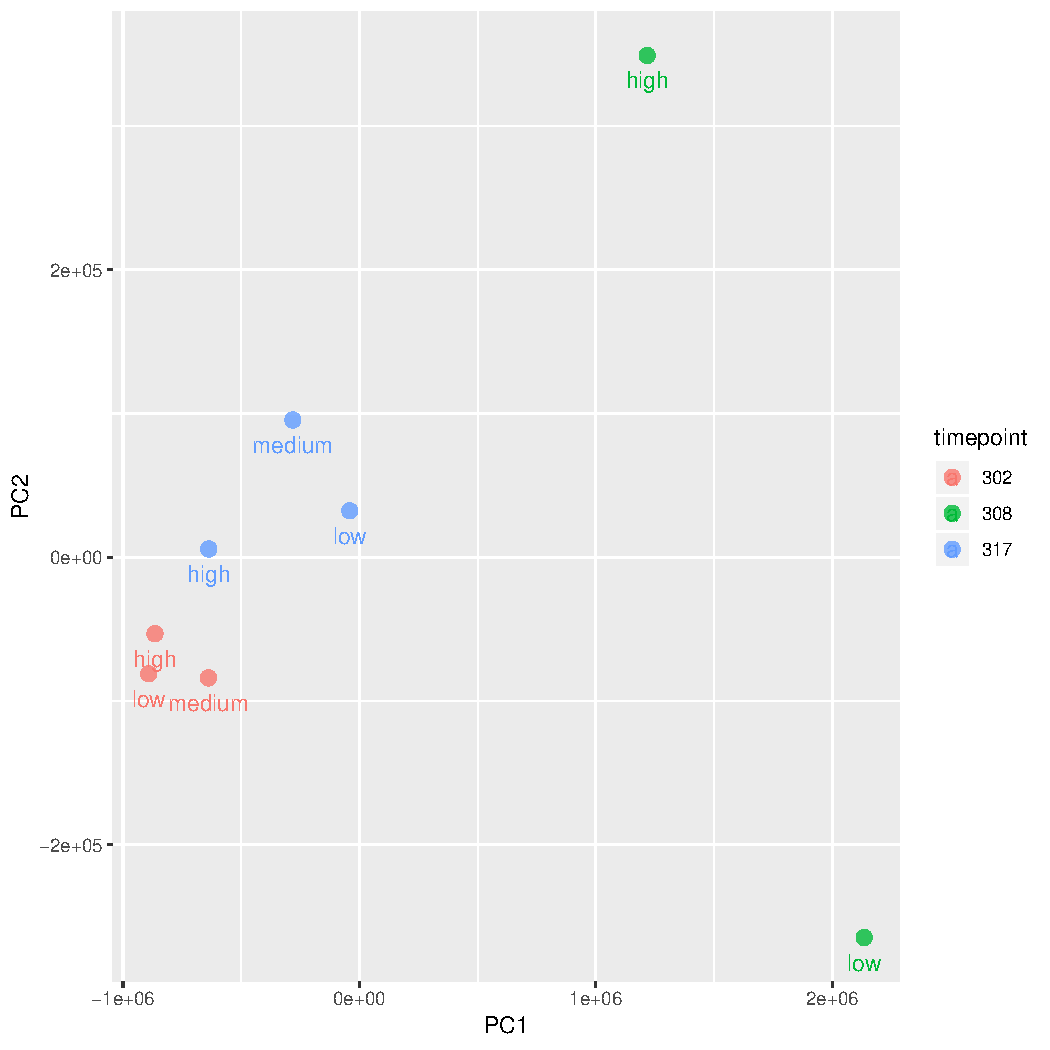
\includegraphics[width=\linewidth, scale=0.5]{figures/intro/intro_tdh2_clustering_timepoints.pdf}
    \caption[Transcriptomes of yeast don't separate out by TDH2 levels]{%
     	\textbf{Transcriptomes of yeast don't separate out by TDH2 levels}
     	We sorted out populations of yeast with high, low and medium levels of TDH2 (3 technical replicates each) as shown in \fref{fig:intro3}. We then extracted RNA and performed RNA-seq. We used PCA to visualize the transcriptomes and find that they don't separate out by the sorted TDH2 levels.
    }
    \label{fig:intro5}
\end{figure}

We counted the transcripts for every expressed gene and performed a PCA analysis on the tnormalized transcript counts. These results are seen in \fref{fig:intro5} The transcriptomes separated out by the day of experiment along PC1. Furthermore, when we looked at individual transcript changes between high and low populations there were very few differentially expressed genes. This result looks like our expected result in \fref{fig:intro4c}. The variability between replicates is higher than the variability within a replicate. Since there were so few differentially expressed genes between teh high and low populations we didn't find any pathway related differences between these populations as well.

While this early experiment of mine was largely a negative result I was still able to get started and thinking about transcriptional variability and its possible functional effects. This experiment was technically challenging since large number of yeast had to be sorted in order to obtain enough RNA for library construction. We had to ensure that the yeast were processed in such a way as to not allow for transcriptional changes after sorting which would remove any real transcriptional differences between the high and low cells. The lessons learnt from this experiment better prepared me for the experiments in Chapter 2 and also inspired me to look for the effect of cell-state on gene expression noise in Chapter 3.

\section{Scope of thesis work}

This thesis consists of two main chapters. In  Chapter 2 I will try to explain the source of phenotypic variability observed within a cell-type. I will test the hypothesis that cells of the same cell-type express different subsets of genes due to stochastic activation of upstream regulators. Specifically, I will test the hypothesis that stochastic expression of transcription factors and stochastic activation of signaling pathways leads to variability between cells of the same cell-type.

In Chapter 3, I aim to understand what determines the noise levels of different genes in the genome. In collaboration with two other graduate students I developed a new genomic technology called SARGENT (Single-cell Analysis of Reporter Gene Expression Noise and Transcriptome) to study noise across genomic locations. Using SARGENT, we integrate the same reporter gene in multiple genomic locations and measure the cell-to-cell variability in expression of this reporter gene using single-cell RNA sequencing. We then attempt to understand the determinants of this noise, after removing the effect of the mean level of expression, using the chromatin state and sequence features at different genomic locations. We also decompose the variability into extrinsic and intrinsic noise, and understand the determinants of these two noise sources. SARGENT also allows us to identify cell-states and quantify the impact of cell-states on noise.

\chapter{Transcription factor fluctuations underlie cell-to-cell variability in a signaling pathway response}
\label{chap:hedgehog}
\vspace{0.2in}

Avinash Ramu\textsuperscript{1} and Barak A. Cohen \textsuperscript{1}

\vspace{0.2in}

\textsuperscript{1} The Edison Family Center for Systems Biology and Genome Sciences and the Department of Genetics, Washington University School of Medicine, USA. 

\vspace{2in}

The manuscript is currently under review and has been uploaded to \textit{Biorxiv} (doi: \href{https://www.biorxiv.org/content/10.1101/2022.11.30.518555v1}{10.1101/2022.11.30.518555}) \cite{ramu2022}.

\newpage

\section{Abstract}
Stochastic differences among clonal cells can initiate cell fate decisions in development or cause cell-to-cell differences in the responses to drugs or extracellular ligands. We hypothesize that some of this phenotypic variability is caused by stochastic fluctuations in the activities of transcription factors. We tested this hypothesis in NIH3T3-CG cells using the response to Hedgehog signaling as a model cellular response. Here we present evidence for the existence of distinct fast and slow responding substates of NIH3T3-CG cells. These two substates have distinct expression profiles, and fluctuations in the activity of the Prrx1 transcription factor (TF) underlie some of the differences in expression and responsiveness between fast and slow cells. We speculate that similar variability in other TFs may underlie other phenotypic differences among genetically identical cells.

\section{Introduction}
Stochastic molecular fluctuations occur within cells \cite{Raser2004-pb,McAdams1997-zq}\cite{Ozbudak2002-dx,Elowitz2002-wn,Raj2006-oo}\cite{Blake2003-yd}. These molecular fluctuations can cause phenotypic variability between genetically identical cells in the same environment. For example, cell-to-cell fluctuations of SCA1 help determine the lineage along which hematopoietic stem cells will differentiate \cite{Chang2008-kv}, and cell-to-cell fluctuations of EGFR and AXL underlie the resistance of rare melanoma cells to chemotherapy \cite{Shaffer2017-ql,Shaffer2018-zl}. Because such molecular fluctuations can have important phenotypic consequences, a key question that needs to be answered is what are the molecular mechanisms underlying cell-to-cell variability within clonal cell populations?

Several mechanisms underlying cell-to-cell variability in gene expression have been identified to date. Some variables that can cause differences between genetically identical cells include cell-cycle stage\cite{Zopf2013-ua}, cellular volume\cite{Kempe2015-xy,Padovan-Merhar2015-cx}, mitochondrial content\cite{Neves2010-vn}, ribosome numbers \cite{Guido2007-rf} and cell state\cite{Topolewski2022-bw,Kiviet2014-vj,Iwamoto2016-wf}. However, there are likely additional mechanisms controlling cell-to-cell variability in gene expression, and the advent of single-cell genomics\cite{Trapnell2015-zd,Eling2019-cr} may provide approaches for identifying these mechanisms.
 
Transcription factors control gene expression and play a vital role in development. Stochastic fluctuations in the activities of TFs can be caused by fluctuations in their expression, localization, or post-translational modification. In this study, we define the activity of a TF in a cell using the mRNA expression level of the TF in that cell. We hypothesize that stochastic fluctuations in the activities of TFs, and the subsequent fluctuations of their downstream target genes, contribute to cell-to-cell differences among genetically identical cells. A key prediction of this hypothesis is that the expression variability of certain TFs, or that of their target genes, will correlate with phenotypic differences between clonal cells. Cells that stochastically express high amounts of a TF’s target genes might behave differently from clonal cells expressing lower amounts of the same genes. Indeed this hypothesis has been tested previously in different systems. For example, it has been shown that stochastic levels of a transcription factor underlies cell fate in Drosophila photoreceptor cells \cite{Wernet2006-rg}. The timing of onset of the transcription factor HLH-2 has been linked to cell fate specification in C. elegans \cite{Attner2019-lh} Competence in bacteria is controlled by the levels of a transcription factor ComK \cite{Samoilov2006-gh}\cite{Suel2006-pw}.  We wanted to test if similar stochastic differences in TF levels could underlie other cell-to-cell differences in phenotype.

We use the cellular response to extracellular Hedgehog (HH) as a phenotype to test these predictions. HH signaling polarizes developing tissues through a signaling pathway that results in the activation of the Gli family of TFs \cite{Kong2019-wo,Briscoe2013-ze,Lee2016-bf}. HH signaling can therefore be measured using cells carrying a genome-integrated Gli-responsive reporter gene \cite{Pusapati2018-gs}. However, we found that even among clonal cells, treatment with HH results in significant cell-to-cell variation in the activation of a Gli-responsive reporter gene. We therefore attempted to identify TFs whose fluctuations might account for these cell-to-cell differences in HH responsiveness using single-cell RNA sequencing (scRNA-seq). We identified fast- and slow-responding subsets of cells characterized by distinct expression profiles that were caused, in part, by stochastic fluctuations in the activity of the Prrx1 TF.  We found that over-expression of Prrx1 was sufficient to speed up the response to Sonic Hedgehog agonist (SAG). Our results support the hypothesis that cell-to-cell phenotypic variation is in part caused by fluctuations in the activities of TFs.

\section{Results}

\subsection{Variability in the HH response}
%figure1
\begin{figure}[t!]  
    \centering
    \phantomlabel{fig:hh_figure1a}
    \phantomlabel{fig:hh_figure1b}
    \phantomlabel{fig:hh_figure1c}
    \phantomlabel{fig:hh_figure1d}
    \phantomlabel{fig:hh_figure1e}
    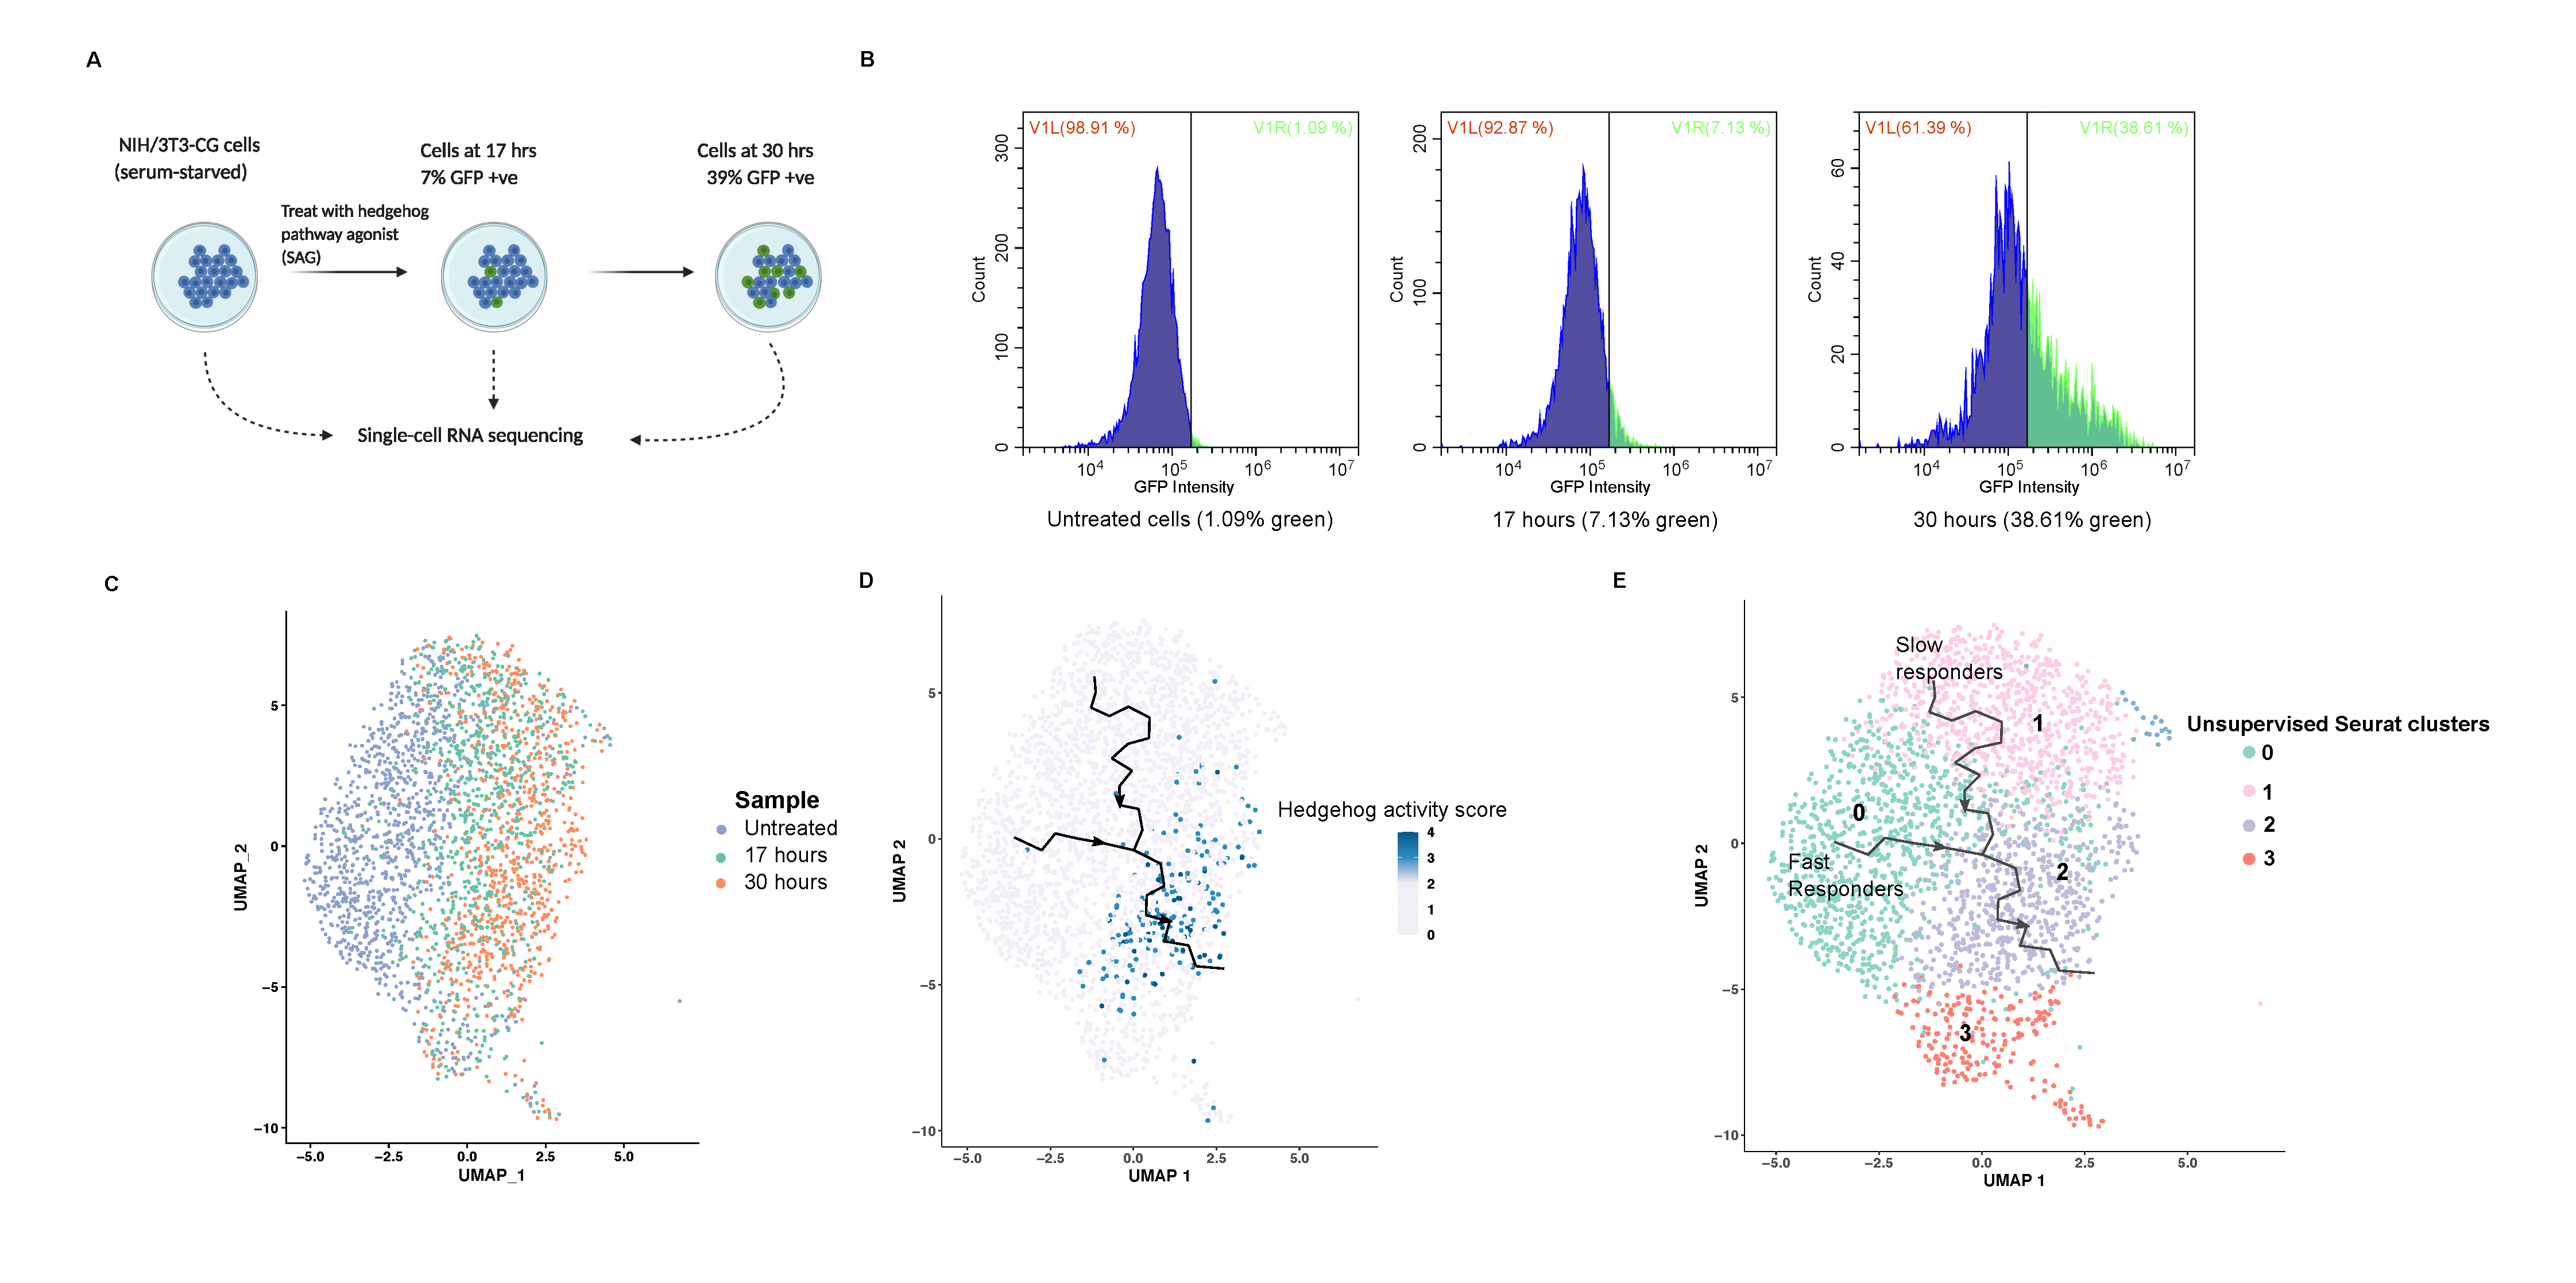
\includegraphics[width=\linewidth]{figures/hedgehog/hh_figure1.pdf}
    \caption[Cells show variability in response to hedgehog stimulation.]{%
        \textbf{Cells show variability in response to hedgehog stimulation.}
        A) Cells were treated with hedgehog agonist SAG for 0, 17 and 30 hours and collected for single-cell RNA sequencing and flow cytometry. (B) Flow cytometry results at 17 and 30 hours indicate that cells show variability in their timing of response, not all same cells respond at the same time (C) Cells clustered with a clear temporal progression of hedgehog response when colored by sample time-point (D) Cells were scored for hedgehog pathway response by looking at mRNA of four canonical hedgehog response genes, responder cells cluster in one part of the graph. Response trajectories were inferred using trajectory analysis software (E) Unsupervised clustering of cells is shown. Cells take two different trajectories to respond to hedgehog pathway activity, one path is fast responding consisting of only cells at zero hours, the other response is from slow responders consisting of cells at 0, 17 and 30 hours.
    }
    \label{fig:hh_figure1}
\end{figure}

We first asked whether clonal cells growing in the same environment show variability in their responses to HH signaling. To address this question, we used NIH3T3-CG cells which are an established model of HH signaling \cite{Pusapati2018-gs,Kinnebrew2019-gt}. Treating these cells with SAG activates the pathway, resulting in elevated activity of Gli transcription factors \cite{Briscoe2013-ze,Lee2016-bf,Kong2019-wo}. This increased activity of Gli is read out by a genome-integrated GFP reporter gene regulated by eight Gli binding sites (\fref{fig:hh_figureS1}). To assess variability in the HH response we treated NIH3T3-CG cells with SAG and monitored the response of the GFP reporter gene by flow cytometry (\fref{fig:hh_figure1a}). Although monocultures of NIH3T3-CG cells are clonal and are grown in the same controlled environment, we detected significant cell-to-cell variability in reporter gene expression in response to SAG (\fref{fig:hh_figure1b}). For example, at 30 hours post SAG treatment only 39\% of cells had activated the reporter gene, whereas by 92 hours most cells responded (\fref{fig:hh_figureS2}). We observed similar variability of response in multiple experimental replicates grown on different days and derived from multiple single-cell clones (\fref{fig:hh_figureS3}).  The data support a unimodal distribution using Hartigan’s dip test\cite{Hartigan1985-zq}. What accounts for the difference between fast and slow responding cells in monocultures with no genetic or environmental variation?

\subsection{Fast and slow responding NIH3T3-CG cells}


We asked whether cells that respond quickly to SAG derive from untreated cells with expression profiles that are distinct from the slow responding cells. To do this, we performed scRNA-seq on cells at 0, 17, and 30 hours after the addition of SAG. We chose the 30 hour time-point since we observed close to maximal cell-to-cell variability in response at this time-point and the 17 hour time-point is about halfway in-between the start of the response and 30 hours. The SAG addition was done in a staggered manner to process all three scRNA-seq libraries in a single batch (Methods, \fref{fig:hh_figureS4}). We first visualized the cells at the three time-points using UMAP (\fref{fig:hh_figure1c}) and performed unsupervised clustering of cells. On the same UMAP plot, we colored the cells for Hedgehog response using four Hedgehog response genes (Methods) and observed a region of the UMAP where the responding cells reside (\fref{fig:hh_figure1d}). We observed similar results when we visualized cells using Principal Components Analysis (PCA) (\fref{fig:hh_figureS5}), but UMAP highlighted the local differences between cells better and captured all the variation in two dimensions.

Next, we used trajectory analysis \cite{Qiu2017-uz,Trapnell2014-ho} to identify the cell states from which slow and fast responders derive. We observed two distinct trajectories after SAG treatment that lead towards cells expressing genes indicative of the Hedgehog response (\fref{fig:hh_figure1d}). Fast responding cells start in cluster 0 and follow a trajectory that leads into cells that express Hedgehog responsive genes at 17 and 30 hours (\fref{fig:hh_figure1e}). Slow responding cells start in cluster 1 and many of these cells remain in the same cluster at 17 and 30 hours, while other slow responding cells follow a trajectory that leads towards but does not reach Hedgehog responding cells. We interpret this result to mean that untreated NIH3T3-CG cells consist of two distinct subpopulations, one that is primed to respond quickly to SAG (fast-responders - cells in cluster 0 of \fref{fig:hh_figure1e}) and another that takes longer to respond (slow responders - cells in cluster 1 of \fref{fig:hh_figure1e}). Very few untreated cells lie outside these two clusters. The fact that these two subpopulations of untreated cells, identified through unsupervised clustering, are in distinct regions of the UMAP plot suggests that their global mRNA expression profiles define the fast and slow responding states.

We used a second trajectory analysis software, Slingshot \cite{Street2018-ak}, to verify the trajectory inferred using Monocle. Both Monocle and Slingshot were both rated accurate trajectory inference tools in a review evaluating different trajectory analysis software \cite{Saelens2019-fq}. We observed similar results with Slingshot (\fref{fig:hh_figureS6}) as we did with Monocle; we find two different trajectories, one starting from the fast responders and another from the slow responders, leading to the hedgehog responsive cells.

One hypothesis that might explain cell-to-cell differences in the timing of the Hedgehog response between the two subpopulations would be transient activation of Hedgehog signaling in the absence of ligand. Cells that are in the midst of transiently activating the pathway would then respond faster to extracellular ligand than the remaining cells. To test this hypothesis, we looked for subsets of cells that expressed targets of Hedgehog signaling. In the unstimulated population we did not observe individual cells with activation of Hedgehog target genes (\fref{fig:hh_figureS7}). Thus, Hedgehog signaling appears to be regulated tightly enough that stochastic activation of the pathway in the absence of ligand is unlikely to account for the cell-to-cell differences in cellular response after the addition of ligand.

\subsection{Differences in cell cycle state do not fully explain fast and slow responding cells}

We next asked whether differences in the cell-cycle state of cells might explain the differences between the fast and slow responding cells. We serum-starve cells prior to hedgehog treatment to synchronize the cells. We used the global expression profiles of serum-starved untreated cells to assign them to different phases of the cell cycle and asked whether fast responding cells were enriched for any specific phase of the cell-cycle. We observed a 1.5 fold enrichment (74.3\% of fast responders vs 50.4\% in the slow responders) of G1 cells in the fast responders compared to the slow responders (\fref{fig:hh_figureS8}). While we found a statistically significant enrichment, the fact that half of slow responding cells were found in G1 suggests that being in G1 is not sufficient to respond faster. To validate the Seurat cell cycle measurements, we measured the \% of cells in different phases of the cell cycle using Propidium Iodide staining after 24 hours and 48 hours of serum starvation (\fref{fig:hh_figureS9a}). The computed percent of cells in different phases of the cell cycle after 24 hours of serum starvation agrees with the Seurat estimated cell-cycle fractions. To further test the effect of the length of serum starvation, we serum starved cells to two lengths - 24 hours and 48 hours. We then used Propidium Iodide staining to look at the \% of cells in different phases of the cell cycle. We observe similar amounts of hedgehog response variability after 48 hours of serum starvation as compared to 24 hours of serum starvation (\fref{fig:hh_figureS9b}) indicating that 24 hour serum starvation is sufficient. We conclude that cell-cycle differences do not fully explain the differences between fast and slow responding cells.
\subsection{Differentially expressed transcription factors and pathways in the fast-responder cells}

We identified genes that are differentially expressed between untreated cells defined as either fast or slow responding (Methods). We focused on the top 300 genes, ranked by fold-change, that were statistically significantly different between the fast and slow populations (Supplementary Data 1). We use these 300 genes in subsequent analyses as markers of the fast responder state. Among the 300 genes, 37 genes are TFs; we decided to focus on the TFs in the differentially expressed genes because we hypothesize that fluctuations in TF activities account for the differences between fast and slow cells. The 37 differentially expressed TFs are shown in \fref{tab:hh_tableS1}. 

We also asked if any biological pathways were among differentially expressed genes between the fast and slow responding cells through a Gene Ontology(GO) analysis (Methods). We observed that the cholesterol biosynthesis pathway is significantly enriched in the set of genes differentially expressed between the two groups (\fref{tab:hh_tableS2}, Enrichment = 28.38, p-value = 1.7e-4, n = 5 out of 13 genes). Cholesterol boosts Hedgehog signaling by serving as a cofactor for Smoothened \cite{Huang2018-iz,Huang2016-er,Kinnebrew2019-gt,Luchetti2016-cd,Radhakrishnan2020-ii}. Increased cholesterol biosynthesis may contribute to the phenotype of fast responding cells. 


\subsection{Slow responding cells pass through the fast state before responding}

Slow responding cells might respond more slowly because they first have to enter the fast responding state from their current state or because they follow a distinct set of cellular states that lead to the Hedgehog response. We distinguished between these two possibilities by examining the set of genes that come on in the slow responders at later time points. Specifically we examined cells from hour 17 and hour 30 in the slow-responding cluster (cluster 1 in \fref{fig:hh_figure1d}) and asked what genes are differentially expressed compared to untreated cells in the same cluster. When the slower responders respond, we observe that they turn on the gene signature of the fast responding cells. At 17 hours these cells express 32 of the 300 fast responder genes (total number of DE genes = 117), and at 30 hours they express 48 of the 300 fast responder genes (total number of DE genes = 196), these are both statistically significant enrichments over random expectation (Hypergeometric test; p-values = 7.9e-27, 1.8e-37). We interpret this result to mean that the slower responders take longer to follow the same trajectory as fast responding cells rather than following a different trajectory.

\subsection{Overexpressing candidate transcription factors partially recreates the fast responder gene signature}

%figure2
\begin{figure}[t!]  
    \centering
    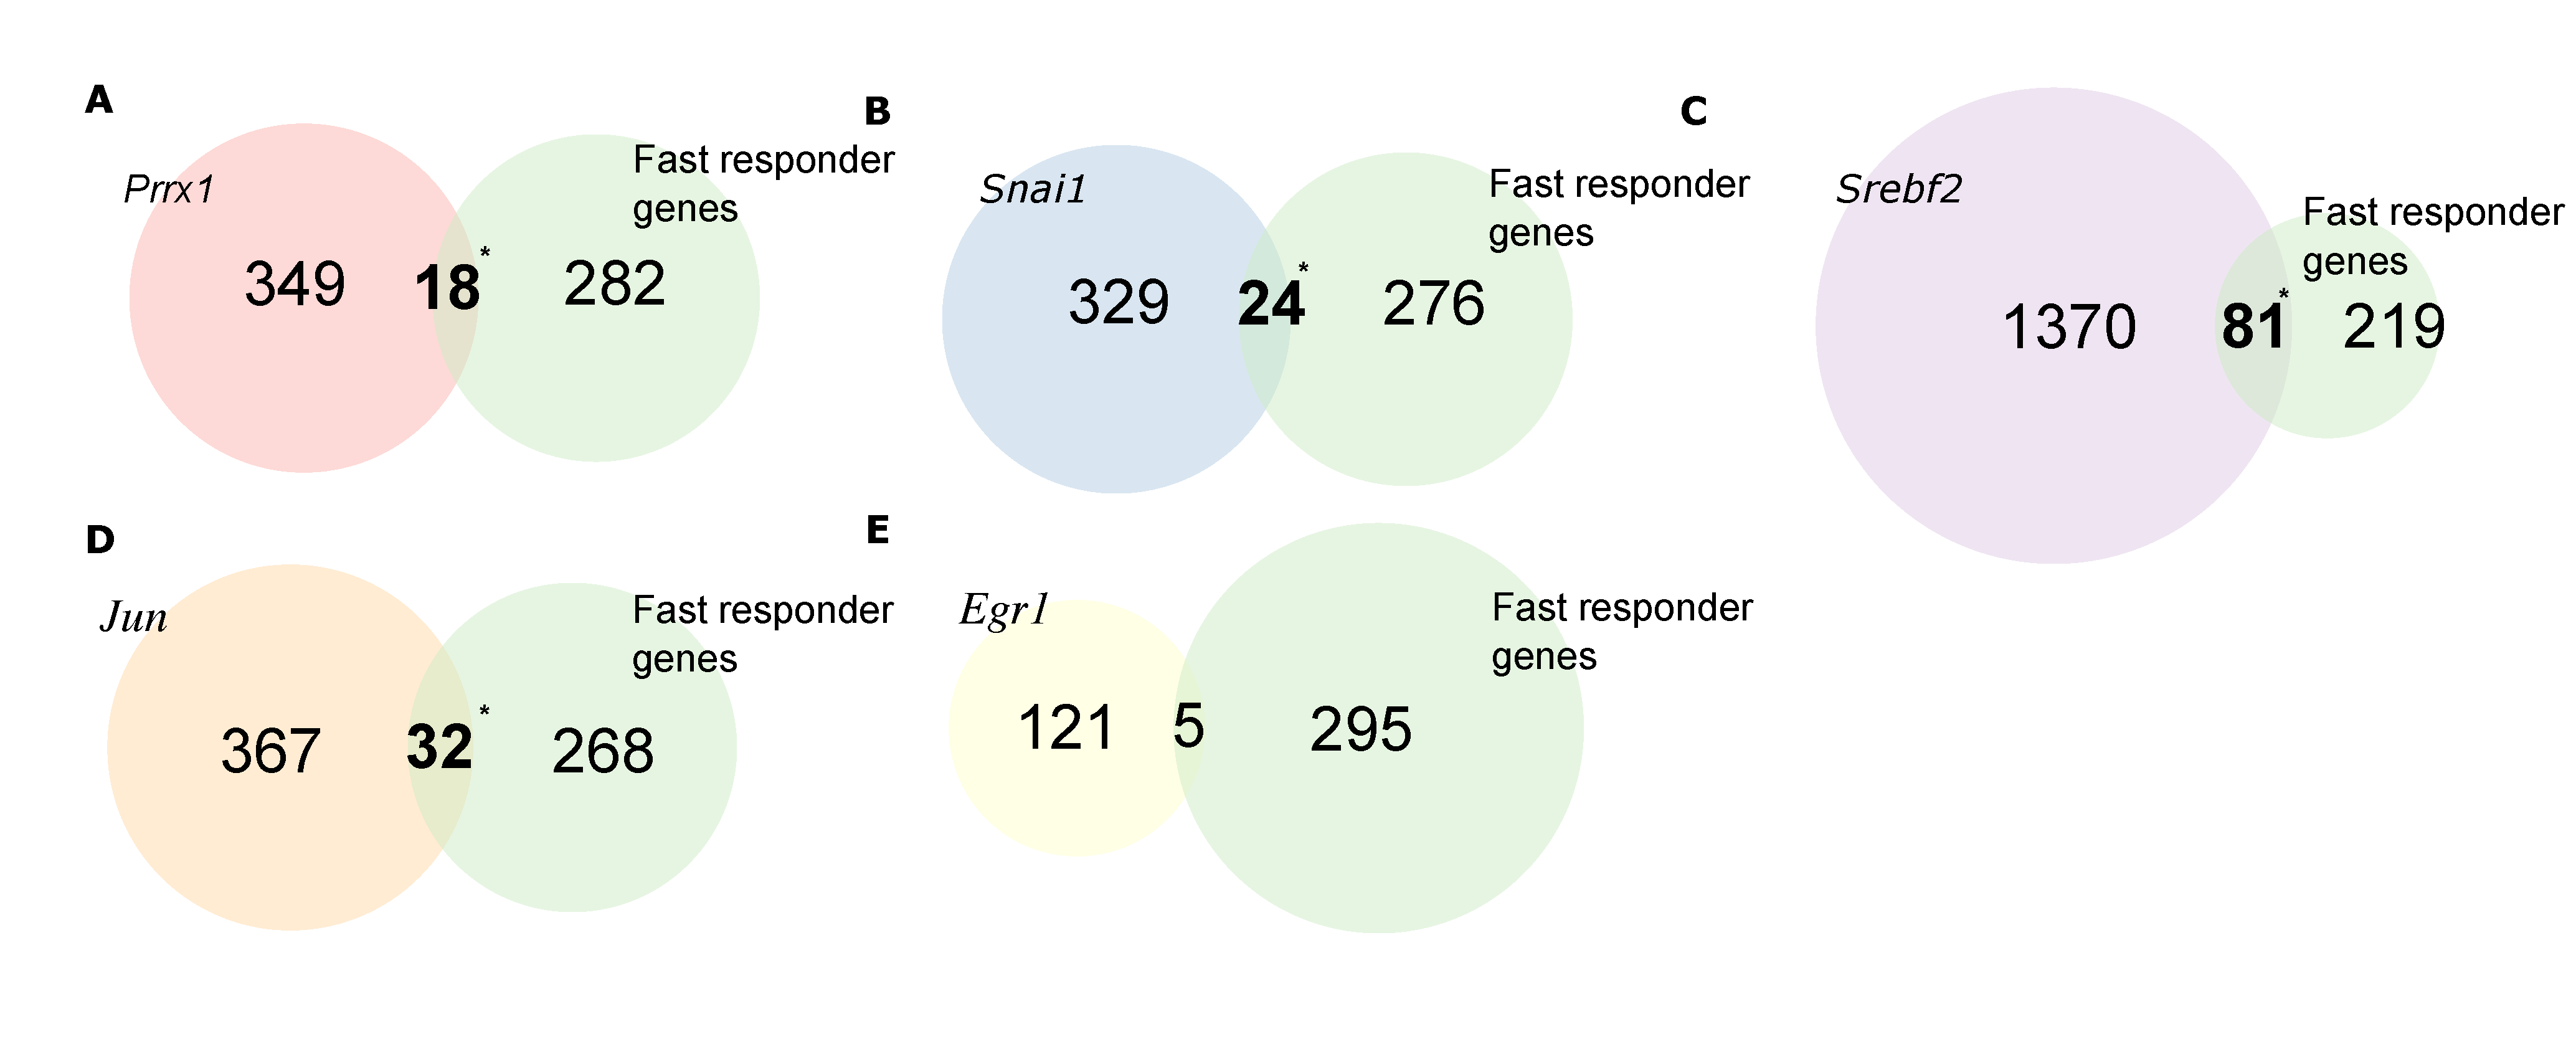
\includegraphics[width=\linewidth]{figures/hedgehog/hh_figure2.pdf}
    \caption[Overexpressing transcription factors partially recreates the fast responder gene expression signature.]{%
        \textbf{Overexpressing transcription factors partially recreates the fast responder gene expression signature.}
        We overexpressed five transcription factors, one at a time, Prrx1 (A), Snai1 (B), Srebf2 (C), Jun (D) and Egr1 (E) using a plasmid transfection assay followed by bulk RNA sequencing. We computed the overlap between the genes that change expression upon transcription factor overexpression(compared to control transfection, n = 3 replicates each) and the 300 genes in the fast-responder gene signature identified using the single-cell data. The (*) indicates a statistically significant enrichment using a hypergeometric test.

    }
    \label{fig:hh_figure2}
\end{figure}

Our results suggest that fluctuations in the activities of a small set of transcription factors and/or the upregulation of cholesterol biosynthesis pathway causes the differences between fast and slow responding cells. To test this hypothesis, we over-expressed these transcription factors and the cholesterol biosynthesis pathway and measured the bulk expression profiles of the resulting cells. We focused on the top three transcription factors based on fold-change in the fast responder cells (\fref{tab:hh_tableS1}): Jun, Egr1 and Prrx1. We also tested the transcription factor Srebf2, the main regulator of the cholesterol biosynthesis pathway \cite{Horton1998-lj}, because this pathway is upregulated in the fast responder cells (\fref{tab:hh_tableS2}). We chose Snai1 as a control transcription factor due to its lower fold change (fold-change 1.21). The expression of the top differentially expressed transcription factors co-localize with the fast responder cell populations (\fref{fig:hh_figureS10}). We designed plasmids encoding the coding regions of Jun, Egr1, Prrx1, Srebf2 and Snai1 under the control of a strong CMV promoter, and with an mCherry gene downstream of the TF to measure transfection efficiency (\fref{fig:hh_figureS11}, \fref{fig:hh_figureS12}). Separately, we used a plasmid containing an mCherry reporter gene driven by a CMV promoter as a transfection control plasmid. We transfected these plasmids into NIH3T3-CG cells and performed bulk RNA-seq. We identified genes that are differentially expressed before and after transfection of each of the transcription factors but not after the control transfection (Supplementary Data 2, 3, 4, 5, 6).

Overexpression of four of the five transcription factors (Prrx1, Snai1, Jun and Srebf2) individually misexpressed a significant number of the fast responder genes (\fref{fig:hh_figure2}; Hypergeometric test: p-values = 9.7e-4, 6.3e-7, 1.2e-10, 1.9e-16), whereas Egr1 overexpression did not (p-value = 0.13). We found that overexpressing Snai1, our control TF with a lower fold-change, also misexpressed a significant number of fast-responder genes indicating that even TFs with lower fold-changes might be involved in creating the fast-responder signature in cells. We found that the union of all four of these TFs (Prrx1, Snai1, Jun and Srebf2) resulted in 115 out of the 300 fast responder gene signature, this is smaller than the naive sum of the individual target genes and indicates overlap in the sets of target genes regulated by the TFs. Overall, we interpret this result to mean that each TF independently regulates a subset of the fast-responder signature.

\subsection{Prrx1 is a regulator of the fast responder state}
%figure3
\begin{figure}[t!]  
    \centering
    \phantomlabel{fig:hh_figure3a}
    \phantomlabel{fig:hh_figure3b}
    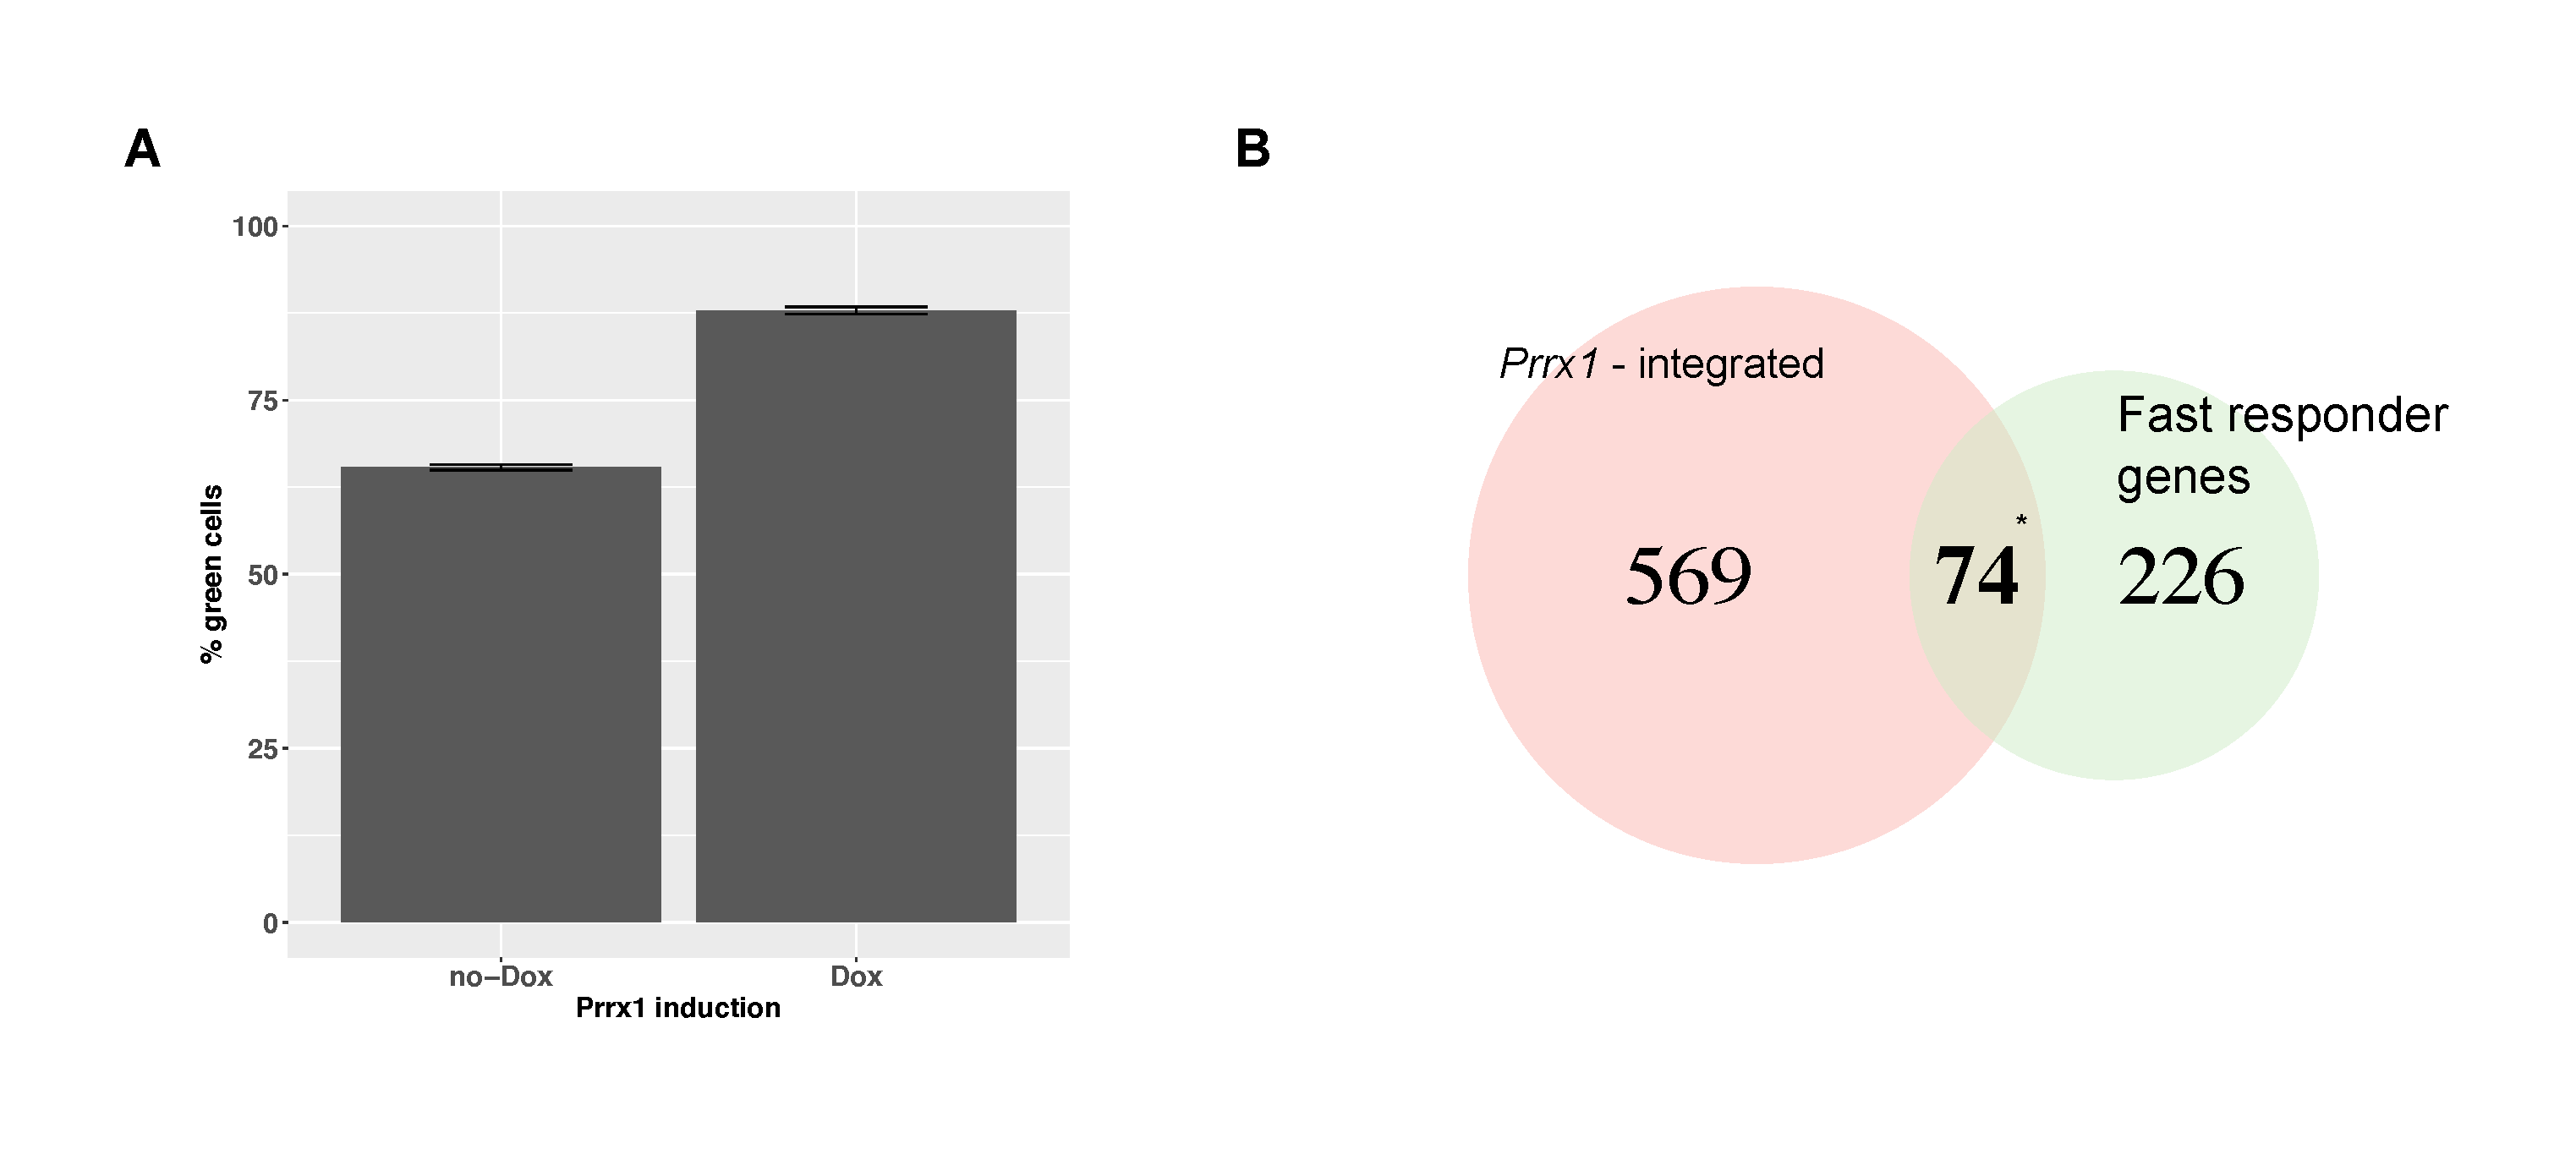
\includegraphics[width=\linewidth]{figures/hedgehog/hh_figure3.pdf}
    \caption[Inducing Prrx1 expression makes more cells fast-responders.]{%
        \textbf{Inducing Prrx1 expression makes more cells fast-responders.} (A) We induced Prrx1 expression in engineered cells by adding Doxycycline prior to performing the hedgehog assay. We compared the hedgehog response of induced cells to cells that were not induced using flow cytometry 32 hours post SAG treatment (n = 3 replicates each). (B) We identified the genes that change expression when Prrx1 is overexpressed by bulk RNA sequencing. We then computed the overlap of these genes with the 300 genes in the fast responder signature.The (*) indicates a statistically significant enrichment using a hypergeometric test. Error bars shown are standard error above and below the mean.
    }
    \label{fig:hh_figure3}
\end{figure}
We next asked whether the overexpression of any of these transcription factors was sufficient to increase the fraction of cells that respond to the Hedgehog signaling pathway. To test this prediction we engineered cells, using lentiviral vectors (Methods, \fref{fig:hh_figureS13}, \fref{fig:hh_figureS14}), carrying Dox-inducible (\fref{fig:hh_figureS15}) versions of Prrx1, Srebf2 and Snai1 integrated into their genomes. This allowed us to compare the fraction of cells that respond to SAG when a TF is either induced or uninduced. We prioritized the list of transcription factors to test since we could not test all of them. We chose Srebf2 since it is the main regulator of the cholesterol biosynthesis pathway which is the top differentially enriched pathway in the fast responding cells (\fref{tab:hh_tableS2}) and showed a statistically significant enrichment. Additionally, we chose Prrx1 and Snai since they showed strong enrichment for competent genes in the transfection assay and because of their roles as developmental TFs.

Inducing Prrx1 expression resulted in more cells responding to the Hedgehog pathway (\fref{fig:hh_figure3a}, \fref{fig:hh_figureS16}, \fref{fig:hh_figureS17}). In the +Dox condition, at 32 hours post SAG treatment, 87.9\% of cells become GFP+, whereas in the -Dox condition 65.4\% of cells become GFP+. We did not observe a difference between the two groups with the induction of Snai1 (\fref{fig:hh_figureS18}). Strong induction of Srebf2 was toxic to cells, and at induction levels that were not toxic we did not observe an increase in the response to SAG  (\fref{fig:hh_figureS19}). From these results, we conclude that Prrx1 plays a role in the regulation of the Hedgehog response.

Bulk RNA-seq profiles from Prrx1 induced cells (\fref{fig:hh_figureS7}) revealed a stronger overlap with fast responding genes than in the plasmid overexpressed cells (\fref{fig:hh_figure3b}; n = 74 out of 300, p-value = 4e-34, enrichment = 5.37 fold). This stronger measured response is likely because in transiently transfected cells only a subset of the cells are expressing Prrx1 whereas in the lentiviral transduced cells all the cells in the population are overexpressing Prrx1. Induction of Prrx1 results in significant enrichment of genes involved in the cholesterol biosynthesis pathway (adjusted p-value = 0.025, enrichment = 10.42, n = 4 out of 13 genes in the pathway). Prrx1 induction also results in the upregulation of Gli2, the primary effector TF of Hedgehog signaling \cite{Kong2019-wo,Briscoe2013-ze,Lee2016-bf}. Gli2 is regulated post-translationally by Hedgehog signaling, so the upregulation of Gli2 in uninduced cells may result in a larger pool of Gli2 protein to activate when the pathway is activated. We observe slight leaky expression in the transduced clone with a fold change of 1.5 X which could underlie some of the higher response in the -Dox condition compared to wild-type cells in \fref{fig:hh_figure1}. A previous study used genome-wide CRISPR knockouts \cite{Pusapati2018-gs} to identify regulators of hedgehog signaling and did not find Prrx1 necessary for Hedgehog signaling. Our results indicate that overexpression of Prrx1 can recreate a substantial part of responder signature, which we interpret as the reason more of these cells respond to Hedgehog signaling.

\subsection{Most cells activate the fast responder gene signature upon Prrx1 induction}
%figure4
\begin{figure}[t!]  
    \centering
    \phantomlabel{fig:hh_figure4a}
    \phantomlabel{fig:hh_figure4b}
    \phantomlabel{fig:hh_figure4c}
    \phantomlabel{fig:hh_figure4d}
    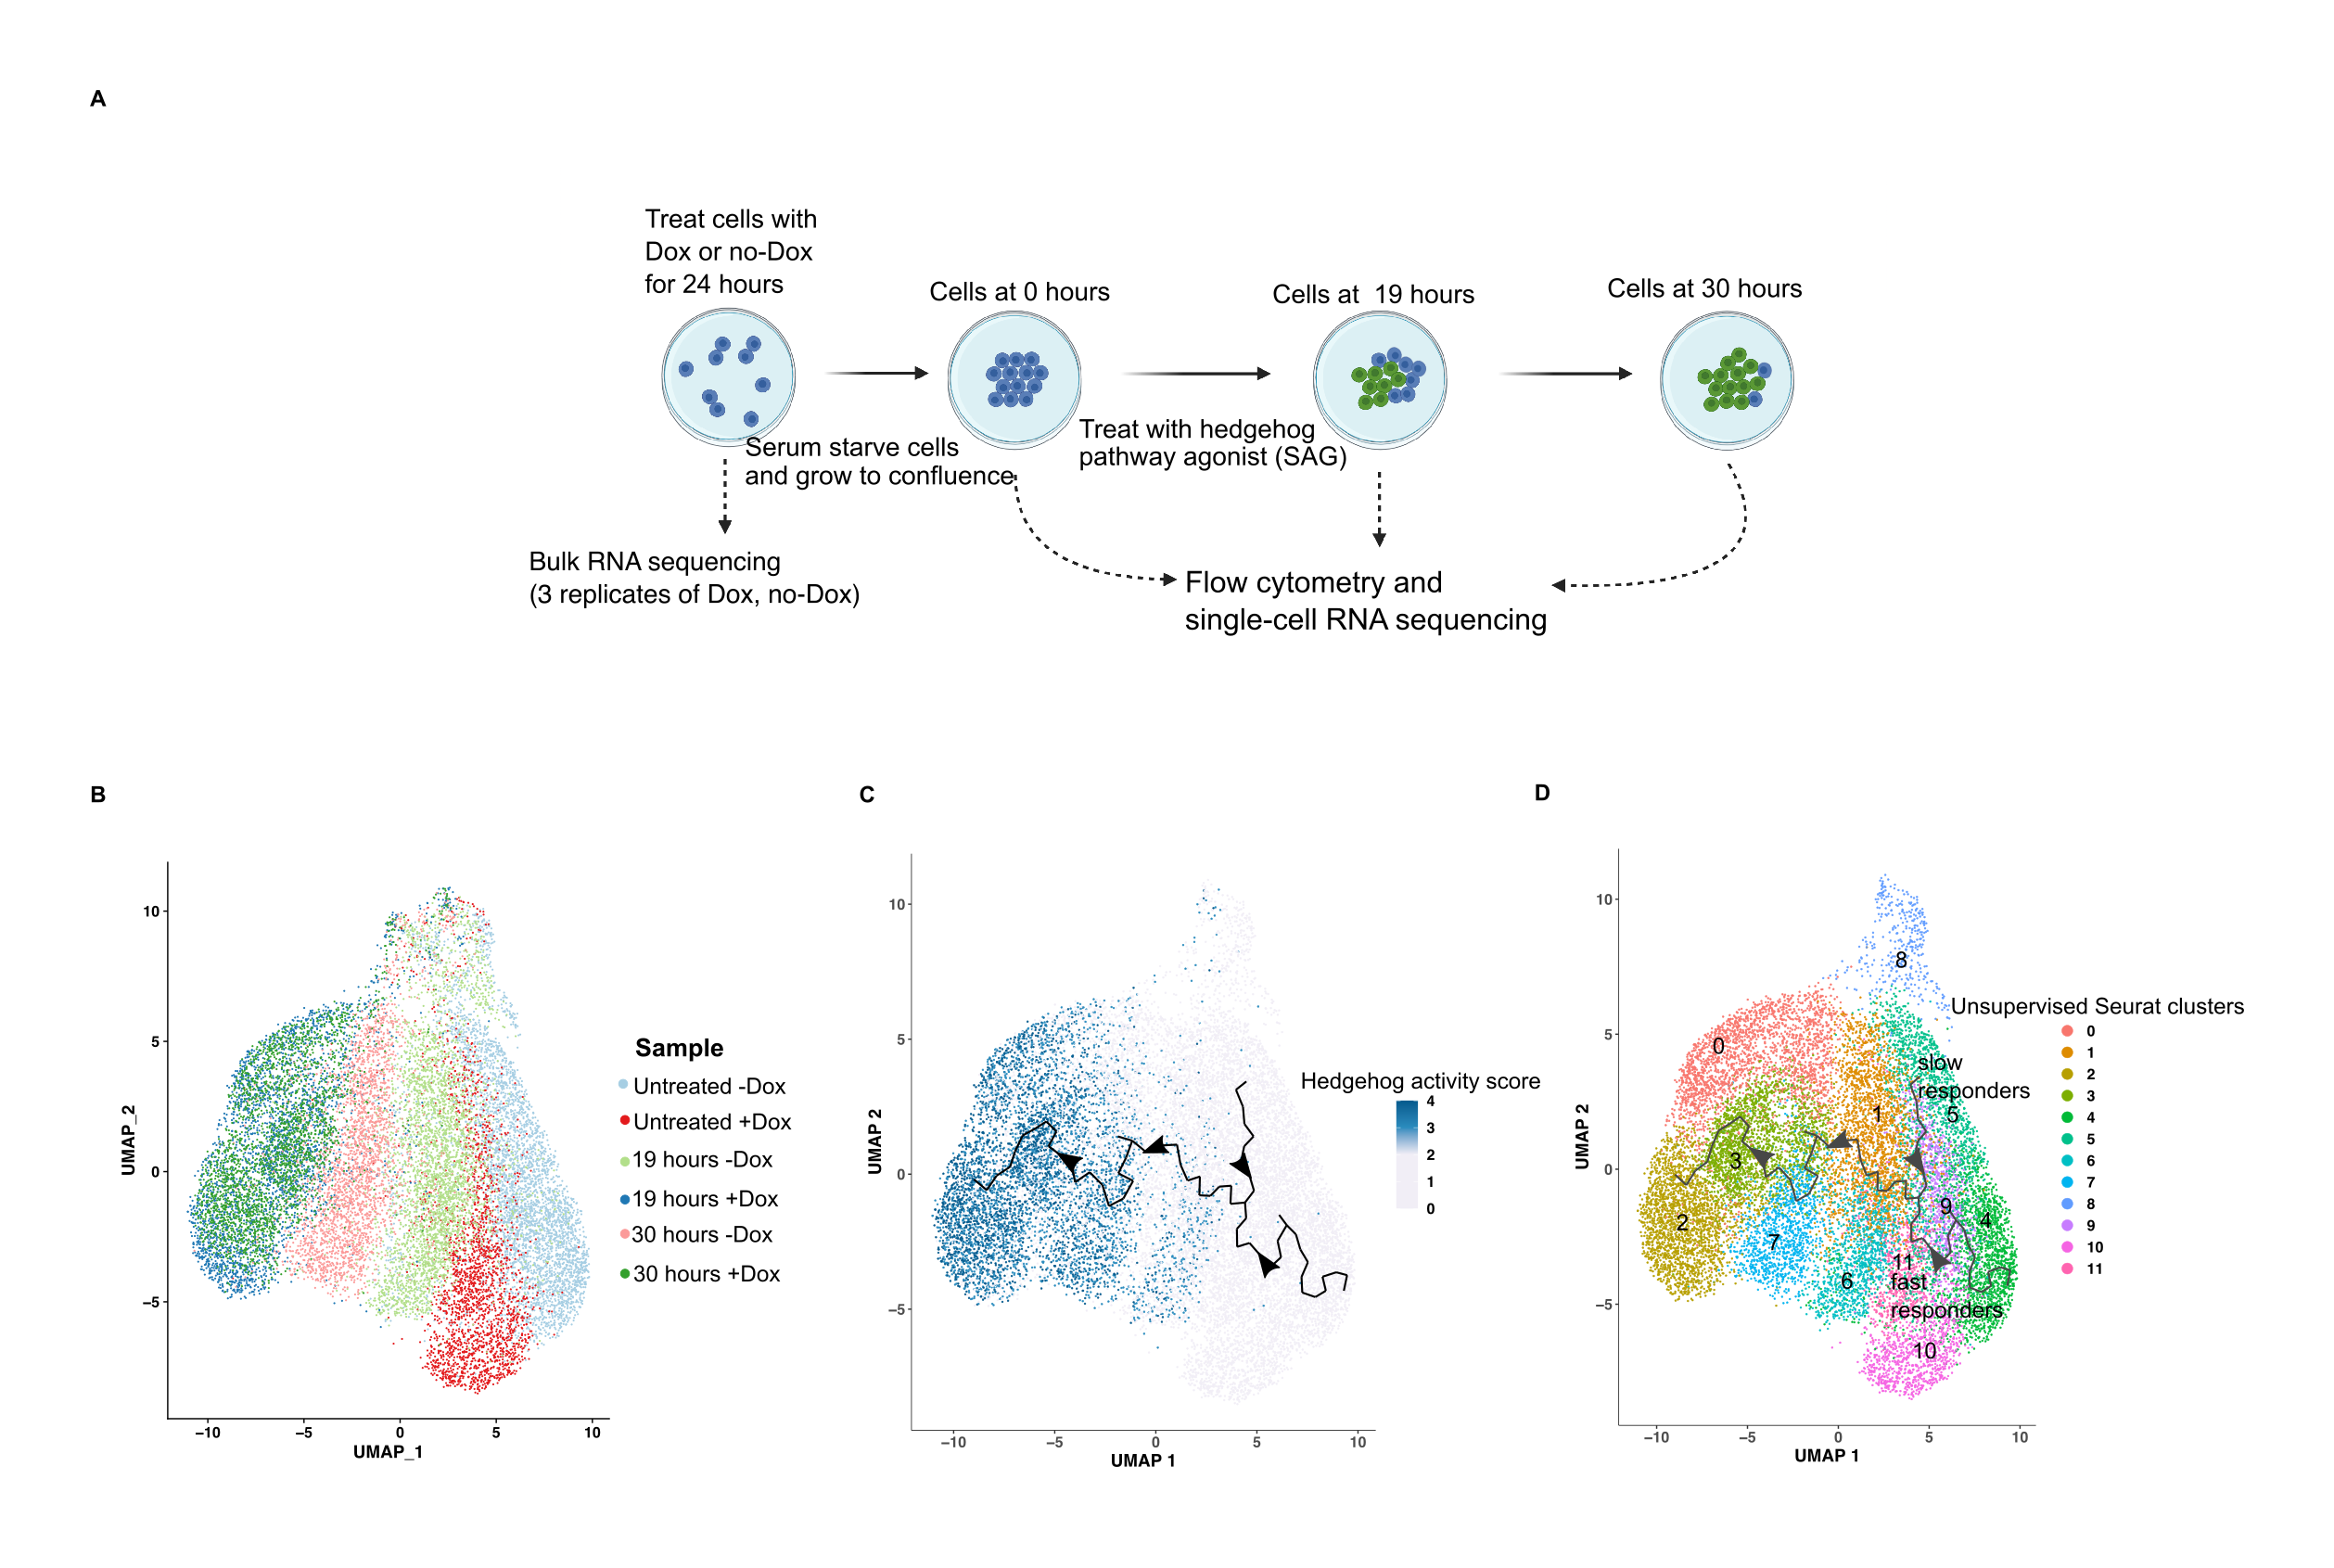
\includegraphics[width=\linewidth]{figures/hedgehog/hh_figure4.png}
    \caption[Prrx1 induction results in faster response trajectory.]{%
        \textbf{Prrx1 induction results in faster response trajectory.} (A) Cells were grown in the absence and presence of Doxycycline for 24 hours, to induce Prrx1 expression, and treated with the hedgehog pathway agonist for 0 (Untreated), 19 and 30 hours. (B) The clustering of the cells from the three time points across the two conditions (C) The inferred trajectory of hedgehog response. Cells were scored and colored for hedgehog pathway response by looking at mRNA expression of four canonical hedgehog response genes (D) The unsupervised clustering of the cells using Seurat. Fast responders and slow responders predicted using a cell-type classifier are shown.
    }
    \label{fig:hh_figure4}
\end{figure}
We next examined the trajectory taken by cells overexpressing Prrx1. We generated scRNA-seq profiles of Prrx1-induced and uninduced cells followed by stimulation with SAG (\fref{fig:hh_figure4a}). We started with the cells carrying the genome-integrated inducible Prrx1 cassette described in the previous section. We grew cells in the absence or presence of Dox, to induce Prrx1 expression, and measured the HH response by flow cytometry. We again observed a larger response in Prrx1-induced cells than in uninduced cells (\fref{fig:hh_figureS20}). We then collected cells at three time points after SAG treatment for both Prrx1-induced and uninduced cells and performed scRNA-seq.

Prrx1 induced cells follow a faster and stronger response trajectory compared to their uninduced counterparts. When Prrx1 is not induced, cells from each time-point again cluster separately, suggesting a steady progression of response to SAG through time (\fref{fig:hh_figure4b}). By contrast, when we induced Prrx1 expression with Dox, cells at the 19 hr and 30 hr time point cluster together, suggesting a faster response to SAG induction (\fref{fig:hh_figure4b}). Overlaying the Hedgehog response on these clusters supports this interpretation as Prrx1-induced cells at 19 hours show similar levels of the Hedgehog response as induced cells at 30 hrs (\fref{fig:hh_figure4c}). However, even at 30 hrs induced and uninduced cells do not cluster together, which suggests that Prrx1 induction results in a stronger response to Hedgehog in cells that do respond. Taken together, these results show that the induction of Prrx1 causes more cells to respond to SAG, and that those cells that do respond, respond faster and stronger than cells that do not express Prrx1.

The trajectory analysis also revealed differences between induced and uninduced cells in the early response to SAG that are consistent with the idea that Prrx1 causes cells to adopt fast-responding expression profiles. Uninduced cells again showed distinct converging trajectories from slow and fast responding states (clusters 4, 5 in \fref{fig:hh_figure4d}), but Prrx1-induced cells respond primarily along the fast trajectory. In addition, the Prrx1-induced cells start from a position along the fast trajectory that is closer to the later time points than the uninduced cells (clusters 9, 10, 11 in \fref{fig:hh_figure4d}), which suggests that they are “further along” the fast trajectory than uninduced cells even before stimulation with SAG. 

We next asked whether inducing Prrx1 creates more fast-responding cells. To detect fast responding cells in this experiment we used a model-based cell-type classifier Garnett \cite{Pliner2019-vn}. We trained the classifier to learn the features of fast-responding and slow responding cells using the cells from the untreated condition shown in \fref{fig:hh_figure1}. We then used the classifier to classify untreated cells grown in the +Dox and -Dox conditions as fast responders and slow responders. In the untreated cells grown in -Dox condition, the classifier classified 19\% of cells as fast-responders, 48\% as slow responders and 33\% of the cells as unknown. The fast responders in this group separate from the slow responders in the UMAP plots and are slightly ahead in the response trajectory even before SAG treatment  (\fref{fig:hh_figureS21A}, \fref{fig:hh_figureS21B}). In contrast, in the untreated cells from the +Dox condition the classifier classified 91\% of cells as fast-responders, 2\% slow-responders and 7\% as unknown (\fref{fig:hh_figureS21C}, \fref{fig:hh_figureS21D}). Thus in the presence of Dox, the majority of cells display the fast-responder expression signature. We infer from this result that inducing Prrx1 generates a fast responder cell-state which makes more cells respond to the Hedgehog agonist, as early as 19 hours.

\section{Discussion}

We hypothesized that fluctuations in the activities of TFs produce transient changes in gene expression that can generate phenotypic differences among clonal cells in the same environment. Consistent with this hypothesis, we showed that distinct gene expression profiles define fast and slow responding states among clonal NIH3T3-CG cells, and that the activities of a small number of TFs accounts for a substantial fraction of the expression differences that define the two states. The idea that these expression profiles cause differences in the response to Hedgehog signaling is supported by the observation that overexpression of Prrx1 is sufficient to generate part of the fast responding expression signature and drive a faster and stronger response to Hedgehog in a larger fraction of cells. However, because Prrx1 only accounts for part of the fast responding expression signature, there must be fluctuations in other TFs\cite{Sigal2006-ds}, or other types of signaling molecules, that generate the fast responding cell state. Much deeper sequencing of unstimulated cells might reveal groups of differentially expressed target genes that could indicate which TFs and signaling molecules are involved, much the same way in which coherent differential expression of the cholesterol biosynthesis pathway suggested the involvement of Srebf2 in the fast responding state. Alternatively, if the transient activation of non-TFs (e.g. receptors, kinases)\cite{Colman-Lerner2005-ln} underlies the fast responding state, then it will be necessary to identify specific changes in gene expression that are diagnostic of changes in the activities of such genes.

We observe parallels between our model underlying variability in the Hedgehog response and other previously described systems where fluctuations of a few key molecules underlie cell-to-cell variability in phenotypic outcomes. For example, differences in the levels of a few apoptotic regulator proteins prior to drug treatment determines how fast cells die in the presence of an apoptosis inducing ligand \cite{Spencer2009-hh}.  Fluctuations of a few resistance genes in cancer cells results in cell states that are resistant to cancer drugs, \cite{Emert2021-ej,Shaffer2020-ff} though the exact mechanisms underlying the emergence of such cell states remains unknown and is hypothesized to involve the fluctuation of multiple upstream transcription factors. In stem cells, fluctuations of a key transcription factor Nanog affect whether cells differentiate or remain in the pluripotent state \cite{Miyanari2012-zv,Torres-Padilla2014-mz}. A recent study using fluorescence microscopy determined that most of the variability in the JAK-STAT signaling response can be attributed to fluctuations in the molecular content of cells \cite{Topolewski2022-bw}. Differences in the amount of transcription factors between cells have been hypothesized to underlie disease due to haploinsufficiency where some cells in a population are unable to express the transcription factor above a required threshold.\cite{Cook1998-es,Kemkemer2002-iw} Single-cell transcriptomic approaches, such as those used in this study, can shed light on the specific molecular differences between cells that result in heterogeneity of response.

Our study also has important implications for improving the efficiency of cellular assays. For example, reprogramming assays can be made more efficient if we understand why some cells are successfully reprogrammed while other cells result in ‘dead-end’ states \cite{Biddy2018-ct,Graf2009-qr,Francesconi2019-ol}. Fluctuations of transcription factors in cells prior to reprogramming might underlie the heterogenous outcome. For example, in hematopoietic progenitor cells, levels of a stem cell marker determine  which lineage a cell differentiates towards \cite{Chang2008-kv}. Isolating cells with different levels of such proteins may improve reprogramming efficiency. Identification of TFs, like Prrx1 in this study, that dampen noise of a system could also aid in the design of synthetic circuits where noise is a significant obstacle \cite{Murphy2010-zb}.

We have inferred the Hedgehog response trajectories using computational methods that look at gene expression similarities between single-cells. A complementary measurement of the trajectory would involve using transcribing molecular barcodes to tag the cells prior to single-cell RNA sequencing \cite{Kong2020-ox}. This approach could reveal how fast cells transition between the slow and fast responder states \cite{Hormoz2016-wo,Stumpf2017-ne,Larsson2021-ub}. We have used overexpression experiments to infer the role of Prrx1 in the fast response. Using GFP fused versions of Prrx1 would help separate the fast responder population from the slow responders and perform functional assays on these subsets of cells. Finally, we have used a widely used cell-culture model of Hedgehog signaling, and how our findings apply to in vivo Hedgehog signaling remains to be tested. 

One future direction of this work will be to determine whether the fast responding state is specific for Hedgehog signaling or if this state makes cells differentially responsive to other signaling pathways and perturbations. We speculate that similar variability in the activities of different TFs may underlie other phenotypic differences among genetically identical cells and experimental approaches similar to ours can be used to uncover this variability.

\section{Materials and Methods}

\subsection{Cell Culture}
We grew NIH/3T3-CG cells and their derivatives in DMEM media supplemented with sodium pyruvate, 10\% Bovine Serum (Gibco 16170078) and 1\% Penicillin-Streptomycin. We grew the cells in an incubator maintained at 37 degrees celsius with 5\% CO2.

\subsection{RNA Sequencing Experiments}
We generated single-cell RNA sequencing libraries using the 10X Single Cell 3’ Reagent Kits v3.1 (10X genomics 1000269). We first released the cells from the cell culture flasks by adding Trypsin 0.25\%. We then prepared a cell suspension by following manufacturer’s instructions and targeting a final capture of 2000 cells for every sample. We then proceeded with library construction as described in the 10X protocol. We sequenced the final libraries at the DSIL and MGI at Washington University in St. Louis. Bulk RNA sequencing was performed using the services of Novogene corporation. Briefly, we extracted total RNA from cells, performed initial QC and shipped it to Novogene where library preparation and sequencing were performed targeting 20 million reads per sample. 

\subsection{RNA sequencing analysis}
We obtained counts for each transcript in each cell by using Cell Ranger version 3.1.0 (https://support.10xgenomics.com/single-cell-gene-expression/software/pipelines/latest/using/count).  We analyzed the cell by count matrix using the standard analysis workflow of Seurat version 3.1.5.\cite{Butler2018-jc,Stuart2019-ra} For quality control, we kept cells that had at-least 10,000 UMIs per cell, had < 20\% of UMIs mapped to mitochondrial genes, and had between 2000 and 8000 genes covered. After QC, for the initial single-cell sequencing experiment we were left with transcriptome measurements for 1,192 cells for the untreated time-point, 797 cells at 17 hours and 899 cells at 30 hours. For the second single-cell RNA-sequencing experiment using the inducible Prrx1 cell-line, under the no-Dox condition we were left with 4532 cells at the untreated time-point, 3726 cells at 19 hours and 2645 cells at 30 hours after QC. Under the Dox condition, after QC we were left with 2362 cells at the untreated time-point, 3014 cells at 19 hours and 2645 cells at 30 hours. 

We performed dimension reduction of single cells using UMAP\cite{McInnes2018-sm}. We identified differentially expressed genes between clusters using the FindMarkers function in Seurat.  We identified pathways that were enriched in the set of differentially expressed genes using the Gene Ontology web resource\cite{Ashburner2000-id,Mi2019-pi,Gene_Ontology_Consortium2021-mx}.

We performed trajectory analysis using Monocle3 version 1.0.0\cite{Trapnell2014-ho,Qiu2017-uz} and Slingshot version 1.4.0 \cite{Street2018-ak}. The Monocle workflow consists of a series of steps. The first step involves pre-processing of the data and dimensionality reduction. We started with the cell by gene matrix that was pre-processed using Seurat and the UMAP dimension reduction results for trajectory analysis. We next identified clusters of the cells using the cluster\_cells method of Monocle. We then used the learn\_graph method to learn a trajectory graph and ordered the cells according to pseudotime using the order\_cells method. We were able to infer directionality on the Monocle trajectory using the timepoint information that the cells come from (each timepoint is a different library on the 10X platform), the arrows in \fref{fig:hh_figure1} go from the earlier time-point to later-time-points as the cells progress through the SAG treatment. For trajectory inference using Slingshot, we used the same cell by gene matrix pre-procesed using Seurat, UMAP dimension reduction results and passed it to the slingshot method. We did not specify the start and end clusters for either Monocle or Slingshot.  More details regarding the parameters used for the various programs are available in the R notebooks made available in the Zenodo repository listed below. 

We computed the hedgehog pathway activity score for each cell by looking at the mRNA expression of four genes - the GFP reporter,  Gli1, Gli2 and Ptch1. For each of the four genes in each cell, we assigned a score of 1 if the gene is detected above background expression level and 0 if not. We then sum over all four genes to obtain a score in the range 0-4 for each cell.

For bulk RNA-sequencing analysis we pseudo-aligned the reads to the mouse reference cDNA using Kallisto version 0.43.0 \cite{Bray2016-hc}. We used the counts from Kallisto to identify differentially expressed genes using DESEQ2 version 1.26.0 \cite{Love2014-lk}. We used a false-discovery rate of 0.05 to annotate genes as differentially expressed across conditions.

\subsection{Enrichment Calculation}
We performed enrichment analysis of the genes that are perturbed when a TF is overexpressed using a hypergeometric test. We detect ~14,000 genes in our single-cell data, out of which there are 300 genes in the fast-responder gene signature. Using a hypergeometric test, for each TF overexpression experiment we ask if the overlap of the 300 genes with the number of genes that change expression upon TF overexpression is a statistically significant enrichment under the null hypothesis of no enrichment. We indicate statistically significant enrichments in the figures with an asterix. We used the hypergeom function in the scipy.stats Python package to compute the enrichment p-values.

\subsection{Hedgehog Assay}
We performed the Hedgehog assay on NIH/3T3-CG cells as previously reported in Pusapati et. al. Briefly, we grew cells to confluence in media containing regular amounts (10\%) of serum. We then switched the cells to low serum media (0.5\% serum) overnight, and treated the cells with the Hedgehog pathway agonist SAG (Tocris Biosciences Part number: 4366) at 100 nM concentration. We measured the amount of fluorescence in the cells on a flow cytometer after allowing for the appropriate time period of response depending on the experiment. For the initial experiment in \fref{fig:hh_figure1a} we collected cells at 17 hours and 30 hours. For the Prrx1 overexpression single-cell experiment we collected cells at 19 hours and 30 hours. For both these experiments, we treated cells that didn’t receive SAG as untreated cells or time-point zero. The time course treatments were done in a staggered manner so that all the cells could be harvested at the same time for single-cell RNA sequencing library preparation. This enabled us to process all the cells in one batch to minimize experimental variability for single-cell RNA sequencing. 

\subsection{Flow Cytometry}
We performed the flow cytometry experiments on a Beckman Coulter Cytoflex S instrument. We performed QC based on manufacturer provided QC beads prior to every experiment. We used the same cytometer gain settings for all experiments. To prepare cells for flow cytometry, we first released cells from culture wells by adding Trypsin and then added appropriate volume of culture media to neutralize Trypsin. We gated cells based on forward scatter and side scatter and measured GFP intensity on the FITC channel. We used a negative control sample (no SAG added) to identify the cutoff for the GFP intensity and measured the proportion of responders as the percentage of cells above this cutoff under different experimental conditions.

\subsection{Plasmid Transfection}
To transfect the plasmids overexpressing the transcription factors we used Lipofectamine 3000 (Invitrogen L3000001) reagent. We used 2.5 ug of DNA per transfection reaction, on a six-well plate, and followed manufacturers instructions for amounts of Lipofectamine and P3000 reagents. We measured transfection efficiency on a flow cytometer using the fluorescence of a reporter gene on the transfected plasmid or a control plasmid transfected in parallel. If we observed sufficient transfection efficiency (> 50\% of cells express transfected plasmid) we extracted total RNA, 24 hours post transfection, from the cells and performed bulk RNA sequencing. The control plasmid used is a mCherry reporter gene driven by a CMV promoter.

\subsection{Lentiviral generation and transduction}
We chose the canonical coding transcripts and sequences for all the genes from UniProt \cite{noauthor_2021-be}. We then cloned the protein coding regions of Prrx1, Snai1 and Srebf2 to the pINDUCER21 Dox-inducible lentiviral vector \cite{Meerbrey2011-ew} using the services of Genscript (Addgene 46948, \fref{fig:hh_figureS6}  and \fref{fig:hh_figureS7}). We used the pINDUCER21 system since it allows us to control the level of over-expression of a gene with precision by adding different levels of Doxycycline to the cell growth media. This construct also has a fluorophore (miRFP670) on it which allows us to isolate cells that contain the integrated construct. The Hope Center at Washington University in St. Louis generated high-titer lentiviruses using the constructs. Detailed lentivirus generation protocol used by the Center is described in their publication \cite{Li2012-if}.

We used the generated virus to transduce the NIH3T3-CG cells and used 4 ug/ml polybrene to maximize transduction efficiency. After 24 hours of cell-growth in the transduction media, we replaced the media with fresh regular media. We used a fluorescent marker of integration to sort single-cells (miRFP670) using a Sony SH800 cell-sorter and grew out single-cell clones that we evaluated for TF induction. 

We evaluated single-cell clones based on induction levels assessed by qPCR. For induction of clones we used Doxycycline (Dox) at a concentration of 500 ng/ml. For transcription factor induction followed by RNA-seq experiments, cells were treated with Dox for a period of 24 hours to induce TF expression. We identified one clone for each transcription factor that offered a good level of inducibility (\fref{fig:hh_figureS8}). We then used these clonal cell lines as a model to study the effect of TF overexpression on the Hedgehog assay. 

To perform the Hedgehog assay, we grew the cells in two different growth conditions - in one condition we added Dox to the media and in the other condition we omitted Dox. We then grew the cells to confluence, for 24 hours, and added SAG to both populations of cells to initiate the Hedgehog pathway response. We used flow cytometry to determine the effect of the overexpression of these transcription factors on the response to Hedgehog stimulation by measuring the GFP fluorescence of the reporter gene on the FITC channel. 

\subsection{qPCR Run and Analysis}
We first extracted total RNA from cells using the Qiagen RNEasy kit(Qiagen 74004). We generated cDNA from the total RNA using the RDRT reagent (Sigma RDRT-100RXN) by following manufacturer's protocol. We then mixed SYBR green PCR master mix(Applied Biosystems 4301955) with 2 ul of cDNA from the previous step, water and primers to set up a standard qPCR run on the QuantStudio instrument (Applied Biosystems). For the transcription factor induction experiments using the transduced cell-lines, we used the no-Dox sample as the baseline for computing the delta Ct value. We used HPRT primers to normalize as a within sample control for TF expression (\fref{tab:hh_tableS3}). We analyzed the results of the QuantStudio run using the Design and Analysis 2 software from Thermo Fisher.

\section{Data Availability}
The raw single-cell and bulk RNA sequencing data from this publication are available from GEO under the accession numbers GSE203134 and GSE206154. Analysis notebooks used for the analysis of single-cell data are available for download at Zenodo: https://doi.org/10.5281/zenodo.6981764



\clearpage
\section{Supplementary Tables}
\begin{supptable}[p]
\centering
\caption{List of top transcription factors overexpressed differentially expressed in the fast responders compared to the slow responders}
\begin{tabular}{ cccc }
\toprule
\textbf{Transcription Factor} & \textbf{Fold-change (fast responders vs slow responders)} & \textbf{Adjusted p-value} \\
\midrule
Jun & 1.54414 & 3.66E-23 \\
Egr1 & 1.41021 & 3.08E-33 \\
Prrx1 & 1.39419 & 1.56E-50 \\
Srsf5 & 1.33099 & 1.53E-45 \\
Maged1 & 1.28932 & 4.09E-36 \\
Asap1 & 1.27863 & 1.15E-25 \\
Fos & 1.26675 & 1.20E-11 \\
Jund & 1.24454 & 2.63E-21 \\
Sub1 & 1.2398 & 1.73E-32 \\
Aebp1 & 1.2163 & 3.99E-16 \\
Tsc22d1 & 1.21429 & 6.90E-15 \\
Nr2f2 & 1.21215 & 1.43E-18 \\
Snai1 & 1.21021 & 4.09E-19 \\
Cebpd & 1.20596 & 0.00216788 \\
Foxg1 & 1.19574 & 1.56E-19 \\
Cited2 & 1.1919 & 8.05E-14 \\
Hlf & 1.19155 & 1.22E-26 \\
Lbh & 1.19117 & 3.12E-20 \\
Ebf1 & 1.18643 & 1.64E-09 \\
Atf5 & 1.18342 & 1.95E-11 \\
Zfp36l1 & 1.17283 & 1.73E-07 \\
Fosb & 1.1675 & 2.45E-12 \\
Nfib & 1.16638 & 1.11E-17 \\
Nfix & 1.16262 & 1.66E-18 \\
Hnrnpd & 1.1563 & 2.40E-17 \\
Drap1 & 1.1537 & 5.51E-19 \\
Sap30 & 0.869089 & 2.41E-11 \\
Nr1d1 & 0.868365 & 1.60E-18 \\
Sqstm1 & 0.865831 & 1.34E-07 \\
Ybx1 & 0.862252 & 3.57E-25 \\
Rnps1 & 0.858557 & 2.88E-17 \\
Tgif1 & 0.848734 & 6.74E-18 \\
Klf9 & 0.819257 & 2.41E-17 \\
Atf4 & 0.817134 & 7.62E-23 \\
Ptma & 0.809741 & 3.20E-33 \\
Tmpo & 0.793335 & 7.15E-26 \\
Ddit3 & 0.533202 & 8.25E-58 \\
\bottomrule
\end{tabular}
\label{tab:hh_tableS1}
\end{supptable}

\begin{supptable}[p]
\centering
\caption{List of signaling pathways enriched in the fast responder cells compared to slow responders}
\begin{tabular}{ p{3cm}p{3cm}p{3cm} }
\toprule
\textbf{Pathway} & \textbf{Genes in fast responder gene signature and in the pathway (Total number of genes in pathway)} & \textbf{Enrichment over random expectation (FDR adjusted p-value)} \\
\midrule
Cholesterol biosynthesis & 5 (13) & 28.38 (1.7e-4) \\
Integrin signaling pathway & 20 (189) & 7.81 (6.2e-10) \\
Ubiquitin proteasome pathway & 5 (65) & 5.68 (4.1e-2) \\
Cytoskeletal regulation by Rho GTPase & 6 (79) & 5.60 (2.3e-2) \\
\bottomrule
\end{tabular}
\label{tab:hh_tableS2}
\end{supptable}


\begin{supptable}[p!]
\centering
\caption{Primer sequences used for qPCR}
\begin{tabular}{ cc }
\toprule
\textbf{Primer} & \textbf{Sequence} \\
\midrule
Prrx1-fwd & GCAGGACAATGACCAGTTGAAC \\
Prrx1-rev & CGTGCGAGATCTTCTCGAAC \\
Snai1-fwd & CGTGTGTGGAGTTCACCTTCC \\
Snai1-rev & GTACCAGGAGAGAGTCCCAGAT \\
Srebf2-fwd & GGACATCGACGAGATGCTACAG \\
Srebf2-rev & TCTGTGGCTCCACCATTGTT \\
Hprt-fwd & CTGGTGAAAAGGACCTCTCGAAG \\
Hprt-rev & CCAGTTTCACTAATGACACAAACG \\
\bottomrule
\end{tabular}
\label{tab:hh_tableS3}
\end{supptable}

\clearpage
\section{Supplementary Figures}

\begin{suppfigure}[p]  
    \centering
    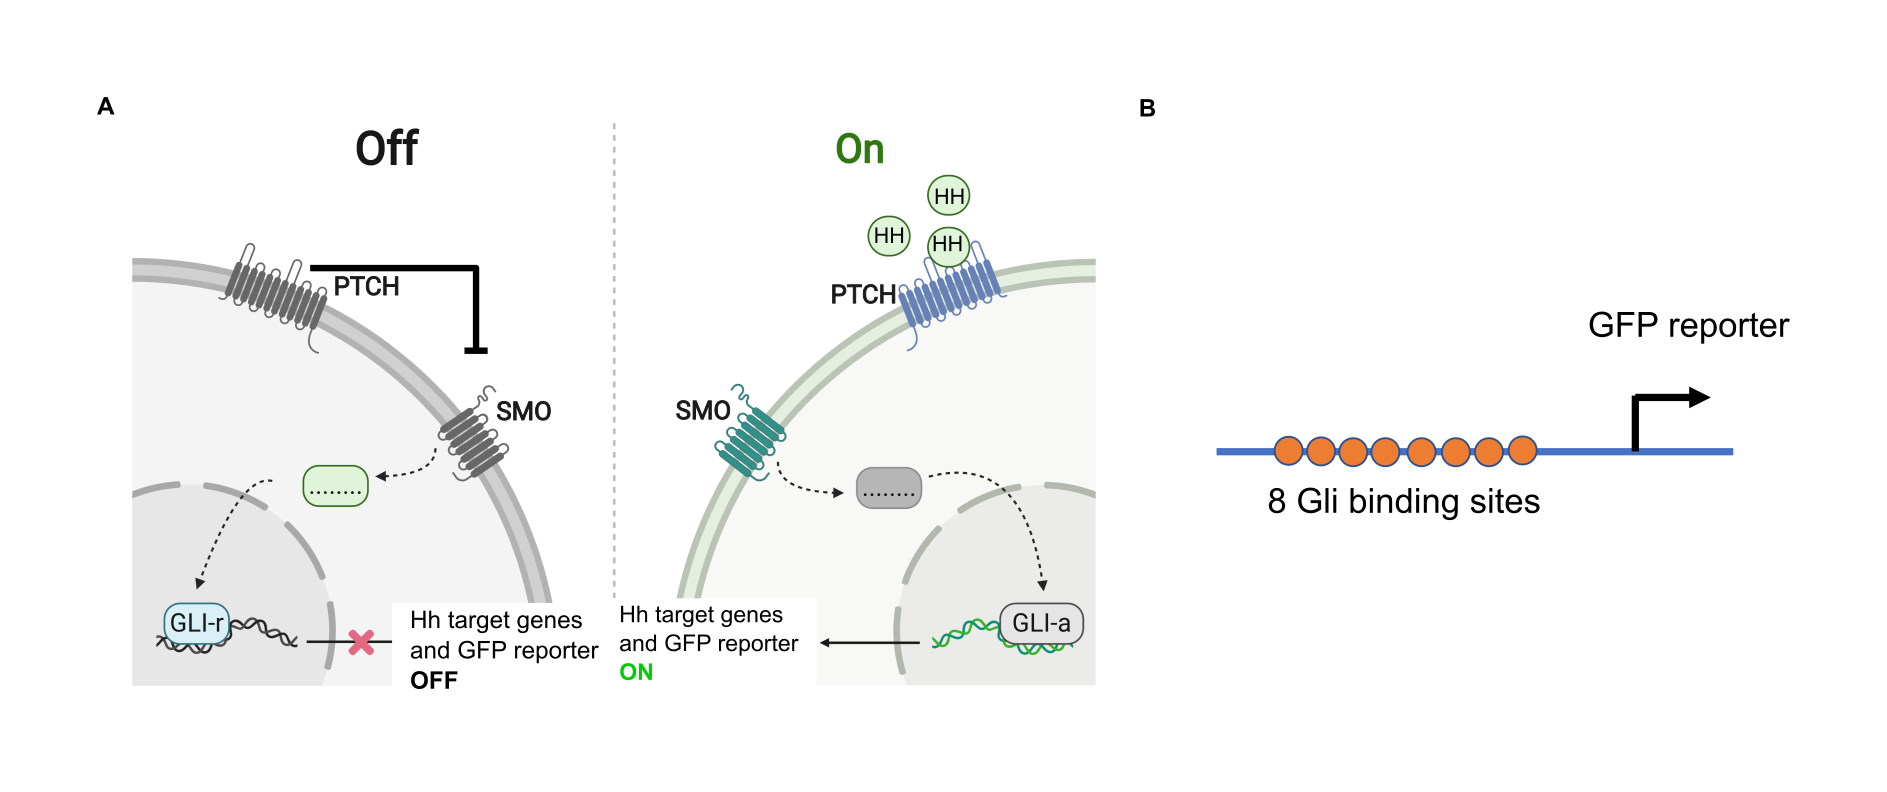
\includegraphics[width=\linewidth]{figures/hedgehog/SuppFigure1.png}
    \caption[A simplified view of the Hedgehog pathway and activation of the GFP reporter]{
        \textbf{A simplified view of the Hedgehog pathway and activation of the GFP reporter}
        (A) In the absence of Hedgehog or SAG the pathway is turned off within a cell, the repression of SMO by PTCH leads to the transcription factor GLI being in its repressed form and it does not turn on the GFP reporter gene. In the presence of Hedgehog or SAG, PTCH no longer represses SMO, GLI acts as an activator and turns on the GFP reporter gene. (B) The cells used in our experiment were generated by Pusapati et al. and contain an integrated GFP reporter gene downstream of eight binding sites of GLI.  
    }
    \label{fig:hh_figureS1}
\end{suppfigure}


\begin{suppfigure}[p]  
    \centering
    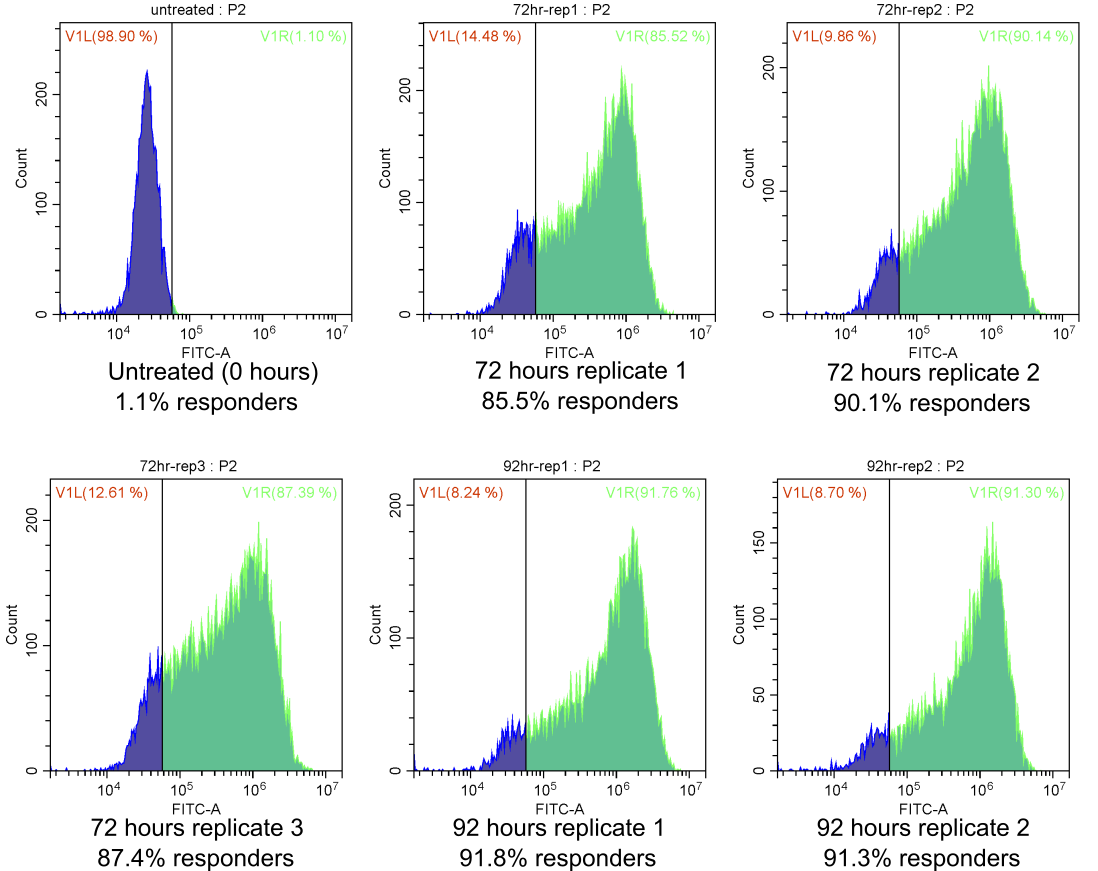
\includegraphics[width=\linewidth]{figures/hedgehog/SuppFigure2.png}
    \caption[Most cells are responders by 72 hours]{
        Flow cytometry results, at 0 (Untreated), 72 (3 biological replicates) and 92 hours (2 biological replicates) post SAG treatment. At 72 hours there are a mean of 87.6\% responders across replicates and at 92 hours the mean fraction of responding cells is 91.6\%.
    }
    \label{fig:hh_figureS2}
\end{suppfigure}


\begin{suppfigure}[p]  
    \centering
    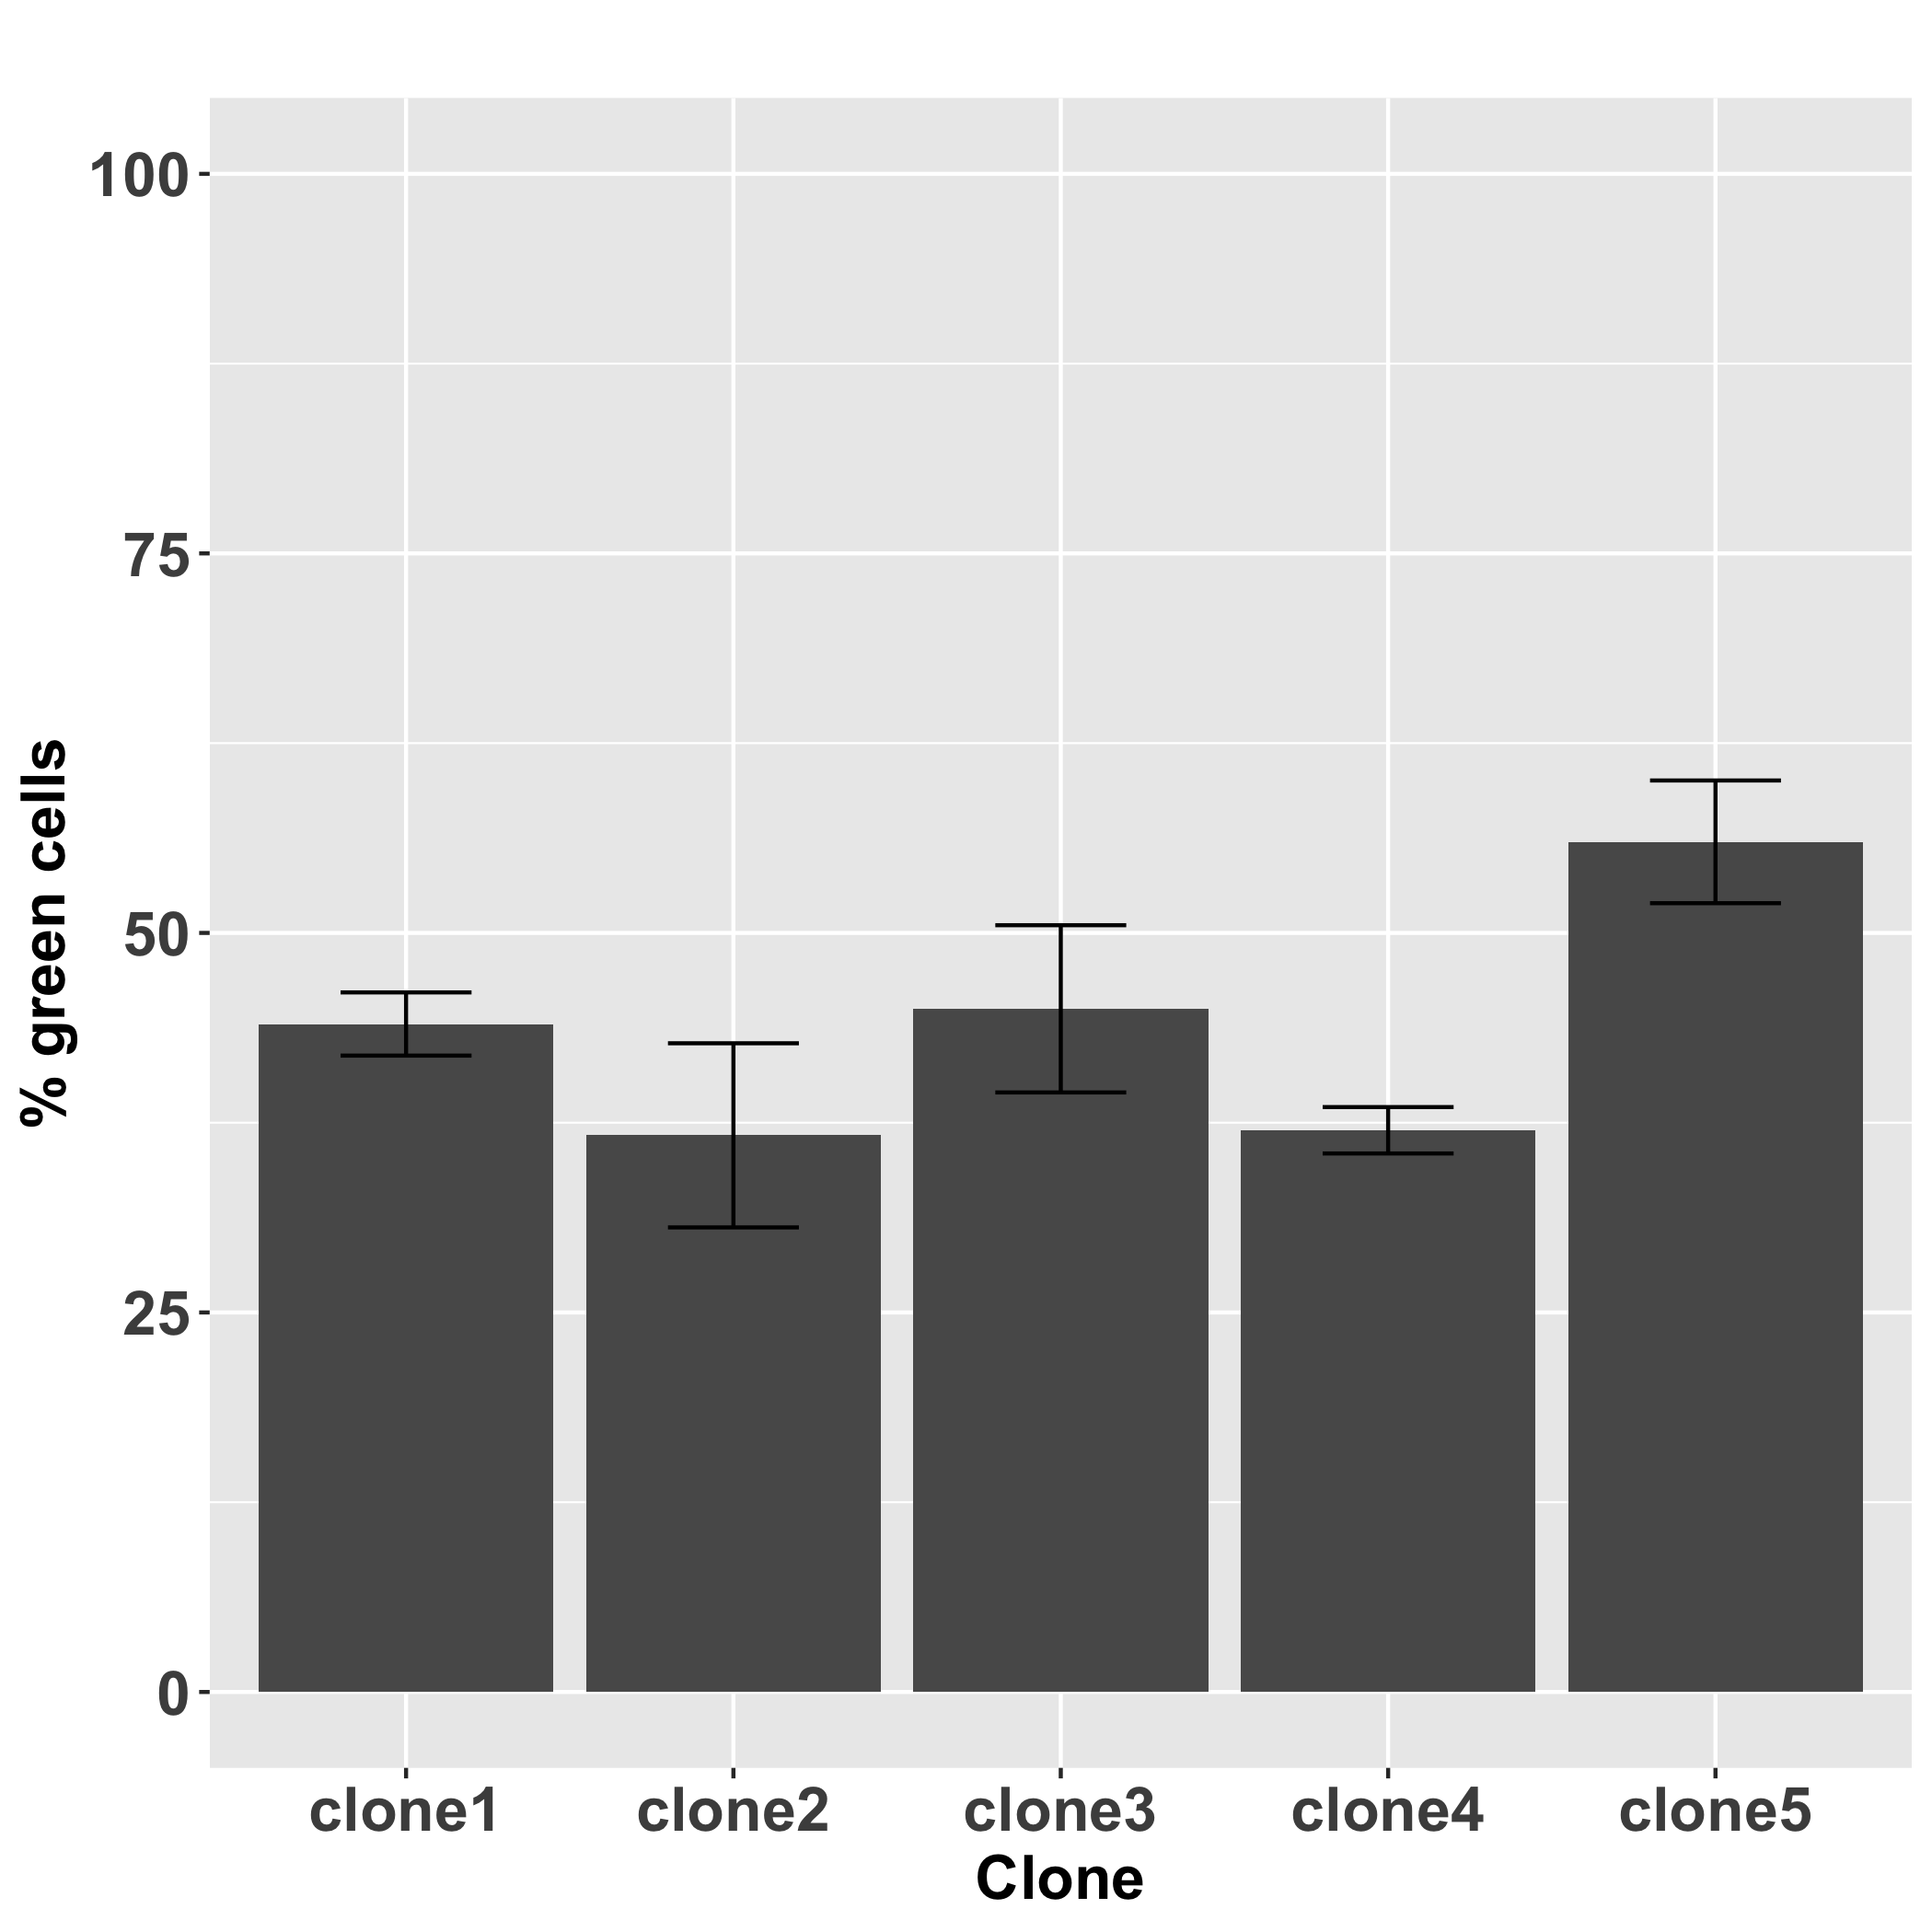
\includegraphics[width=\linewidth]{figures/hedgehog/SuppFigure3.png}
    \caption[Variability in multiple single-cell clones of NIH3T3-CG wildtype]{
        We grew out multiple single-cell clones from wildtype NIH3T3-CG cells and measured the percentage of cells that respond after treating the cells with the hedgehog protocol at the 30 hour time-point. Error bars shown are standard error above and below the mean.  
    }
    \label{fig:hh_figureS3}
\end{suppfigure}

\begin{suppfigure}[p]  
    \centering
    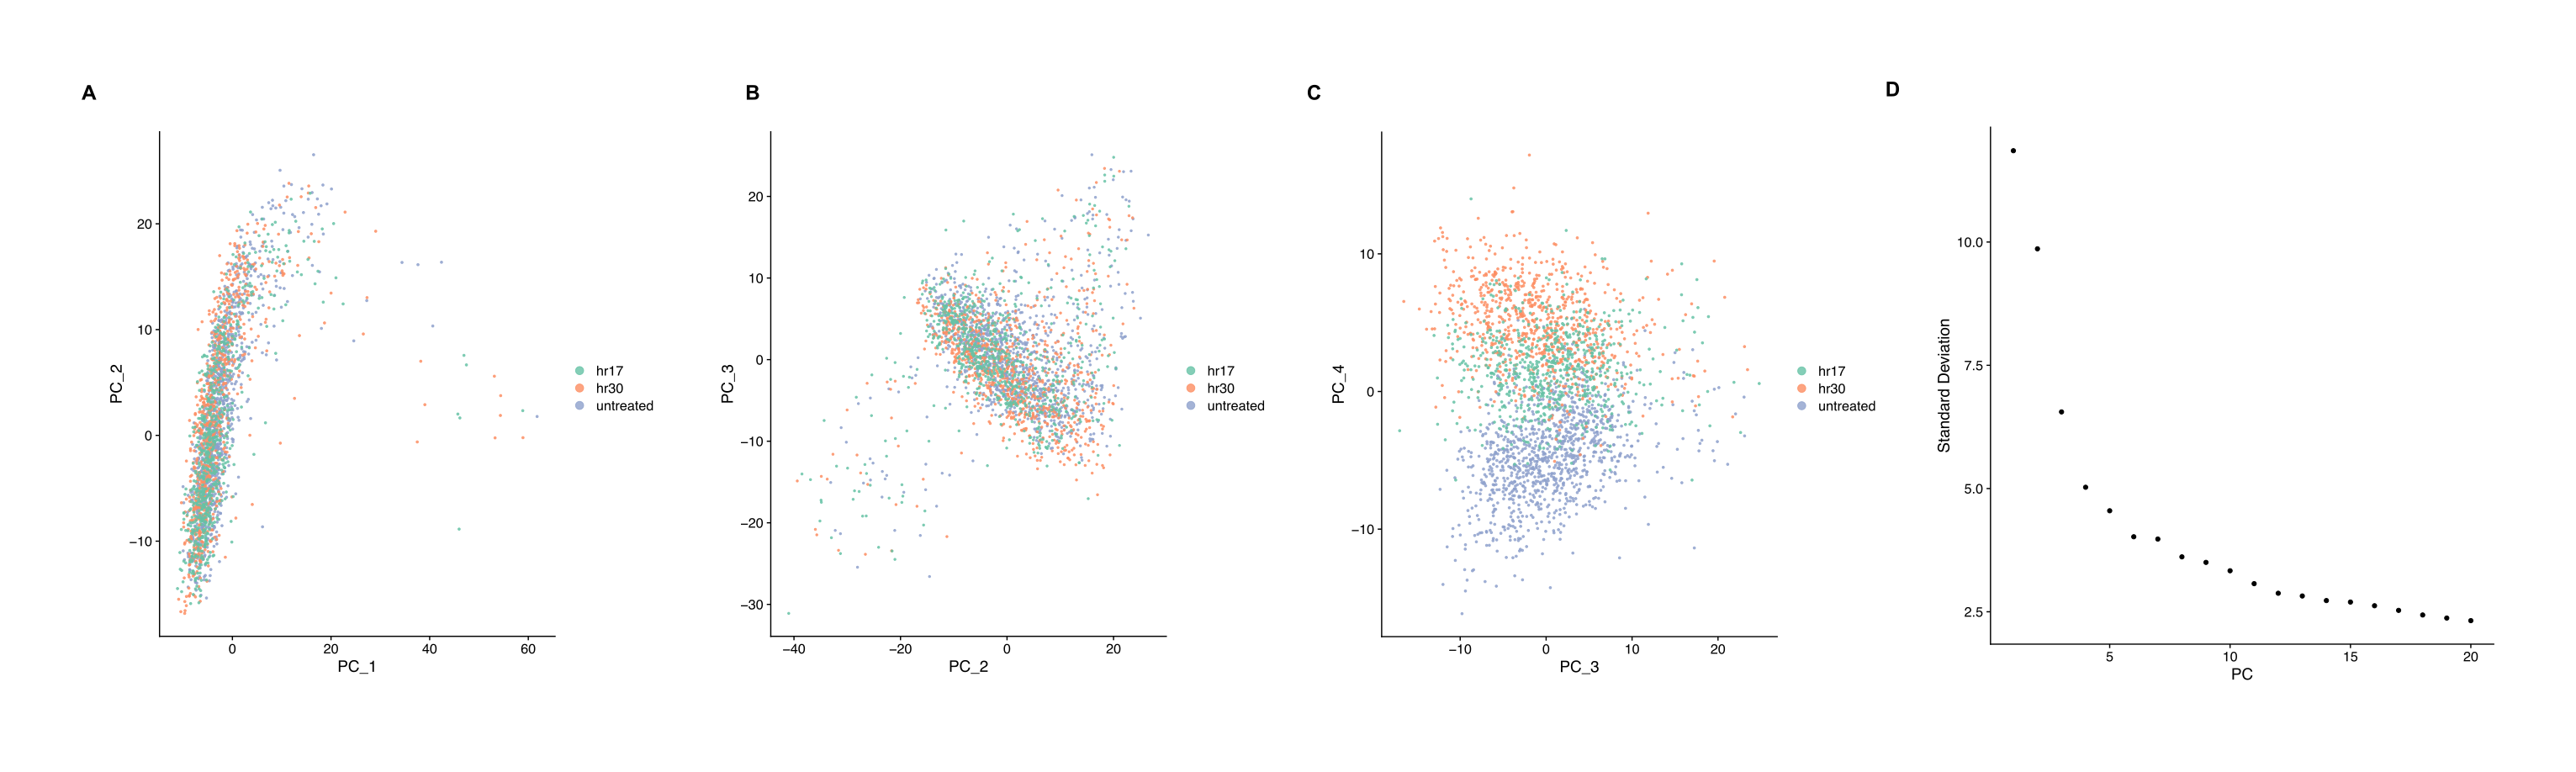
\includegraphics[width=\linewidth]{figures/hedgehog/SuppFigure4.png}
    \caption[No evidence for batch effect]{
        We see no evidence for batch effect since all the three samples were processed in a single batch. We plotted principal components for all the cells shown in \fref{fig:hh_figure1}. Only PC4 (C ) separates out the samples, and this separation is expected based on genes that turn on and off in a temporal manner in response to hedgehog. (D) shows the standard deviation explained by each principal component.  
    }
    \label{fig:hh_figureS4}
\end{suppfigure}

\begin{suppfigure}[p]  
    \centering
    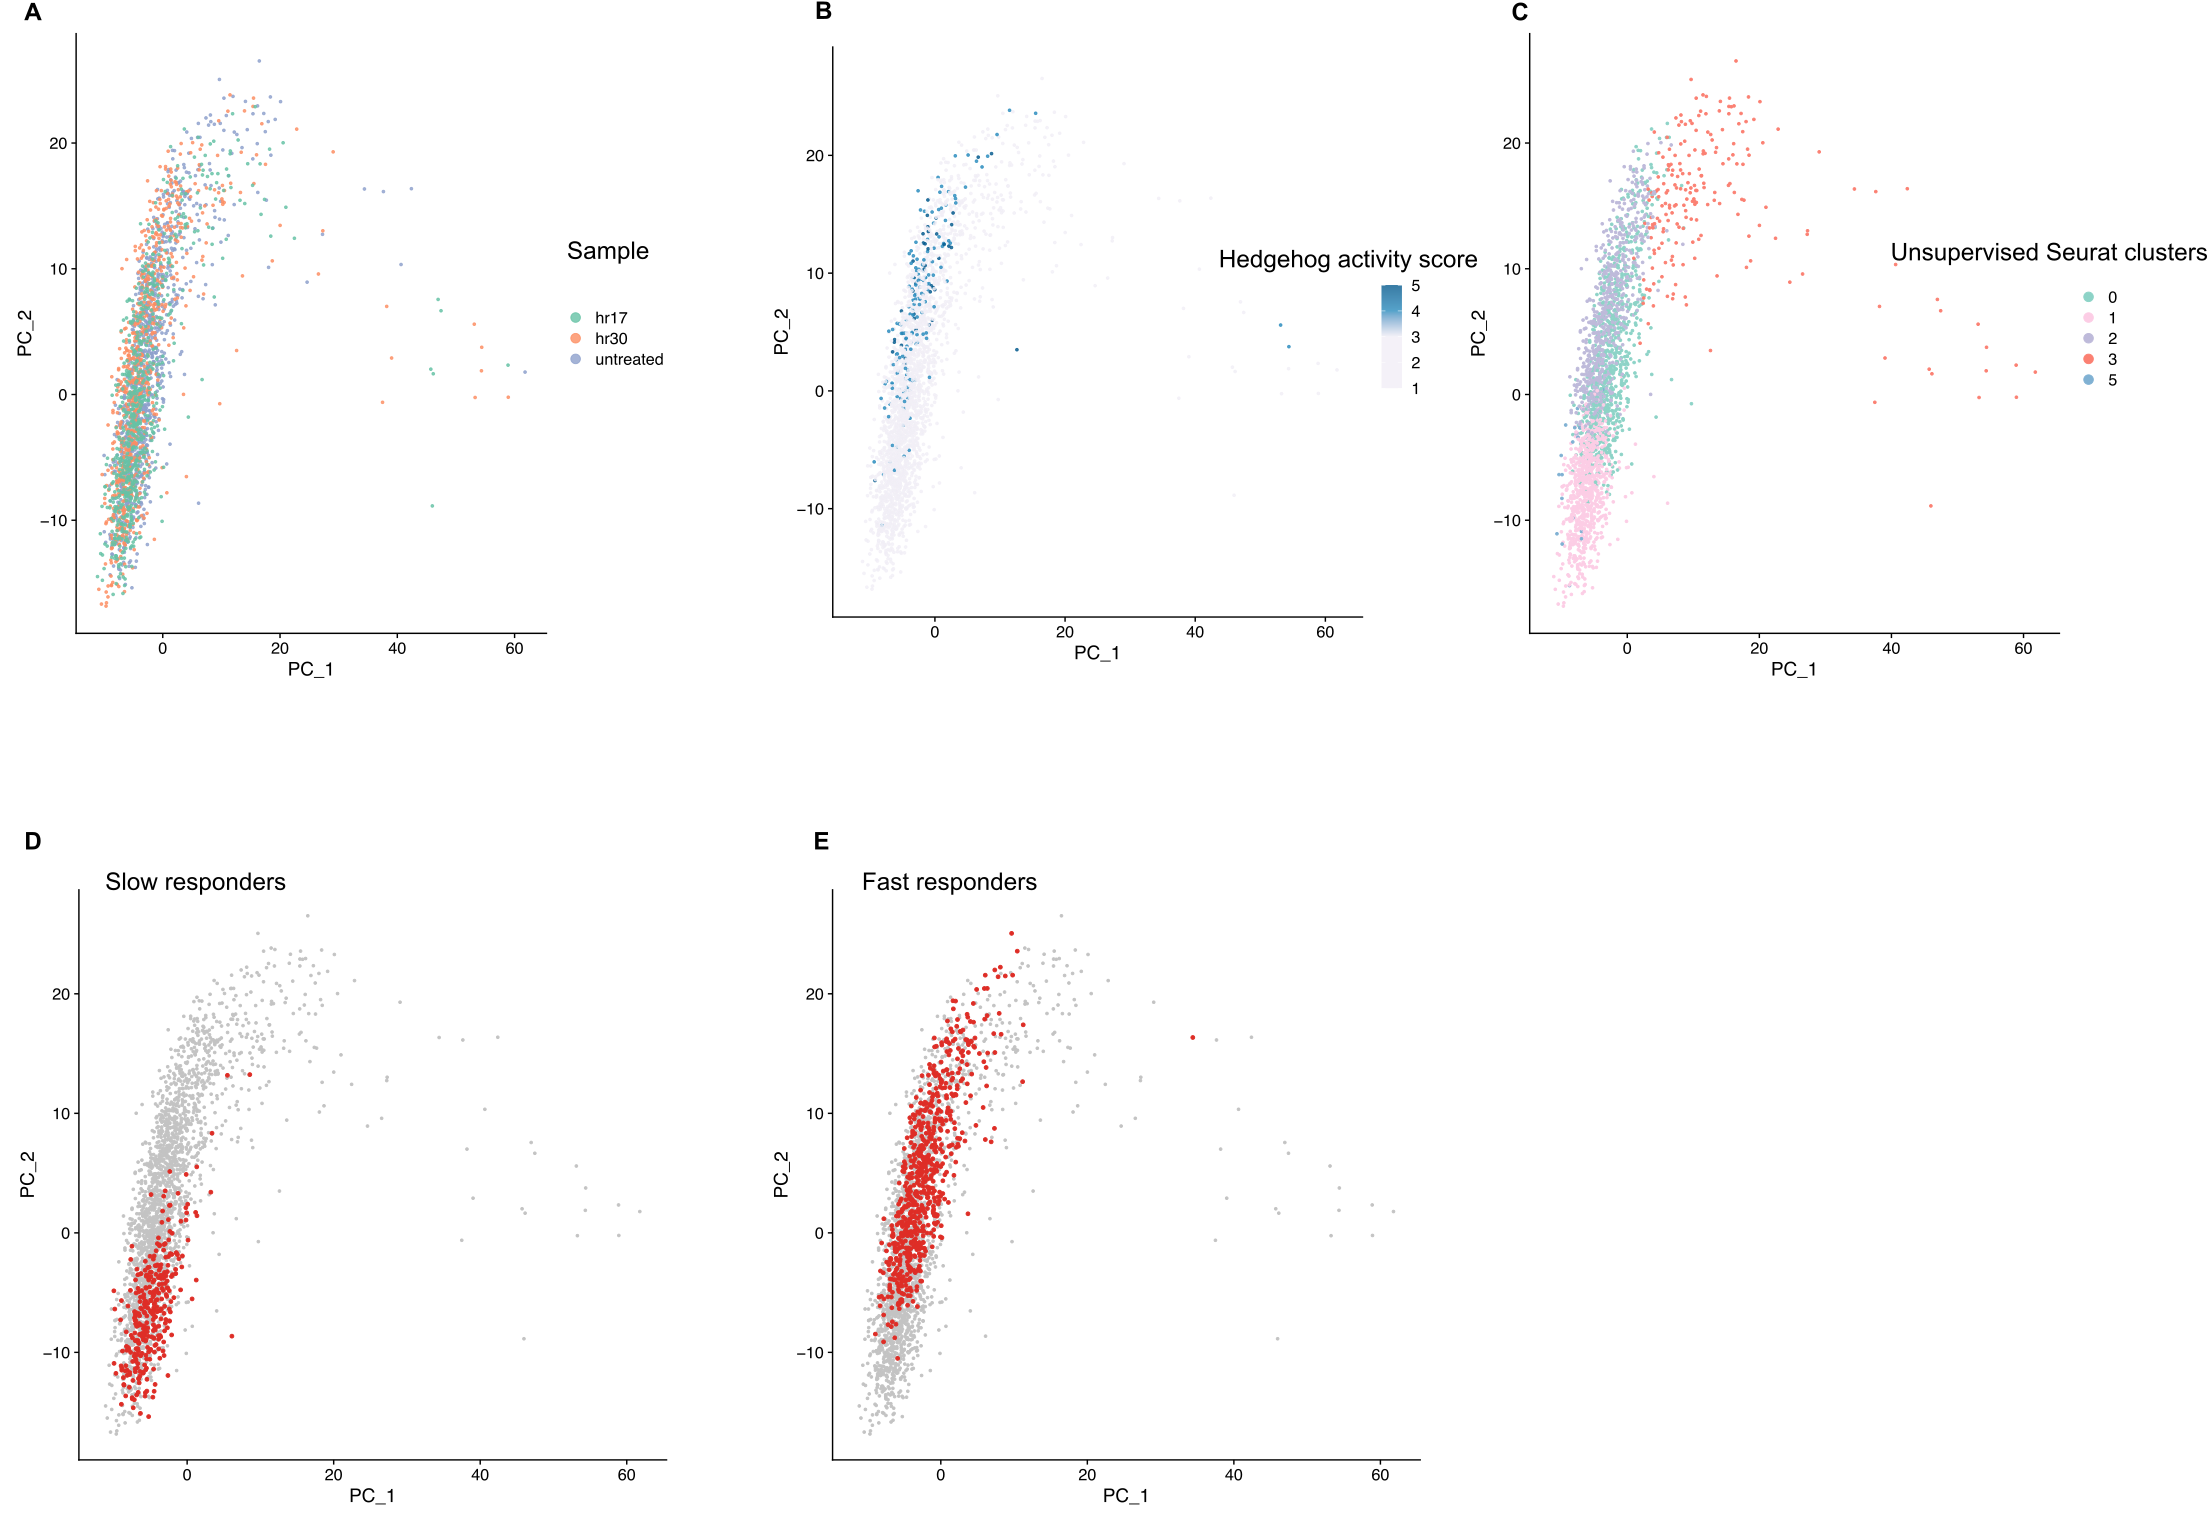
\includegraphics[width=\linewidth]{figures/hedgehog/SuppFigure5.png}
    \caption[PCA visualizations are similar to UMAP]{
        Visualizing cells with PCA shows similar results as visualizing with UMAP. We performed PCA on the cell by gene matrix and plotted the first two principal components for each cell. We colored cells by sample (A), hedgehog activity score (B) and unsupervised Seurat clusters (C ). We highlighted the slow responders (D) and fast responders (E)  identified in \fref{fig:hh_figure1} on the PCA plot and see that they separate out on the principal components plot.
    }
    \label{fig:hh_figureS5}
\end{suppfigure}

\begin{suppfigure}[p]  
    \centering
    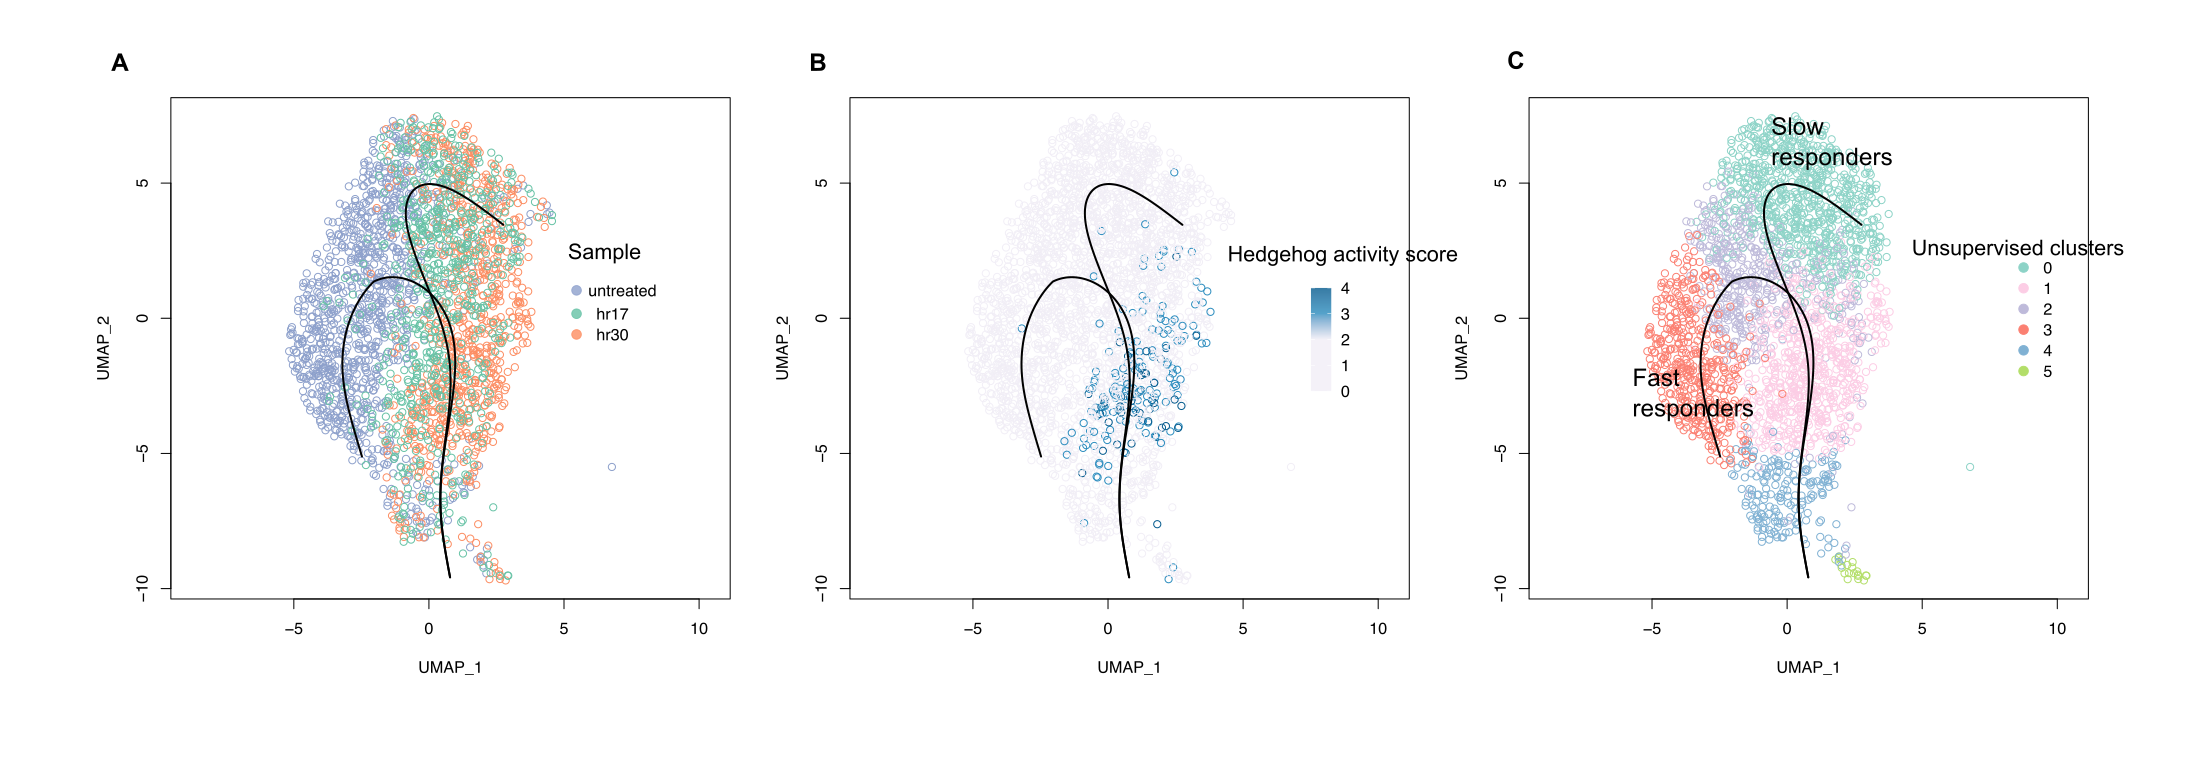
\includegraphics[width=\linewidth]{figures/hedgehog/SuppFigure6.png}
    \caption[Slingshot trajectory analysis results]{
        We used a second trajectory analysis tool Slingshot. Similar to results from Monocle in \fref{fig:hh_figure1}, cells take two different trajectories in their response to SAG. We colored the cells by sample (A), hedgehog activity score (B) and unsupervised Seurat clusters (C ) as in \fref{fig:hh_figure1}. 
    }
    \label{fig:hh_figureS6}
\end{suppfigure}

\begin{suppfigure}[p]  
    \centering
    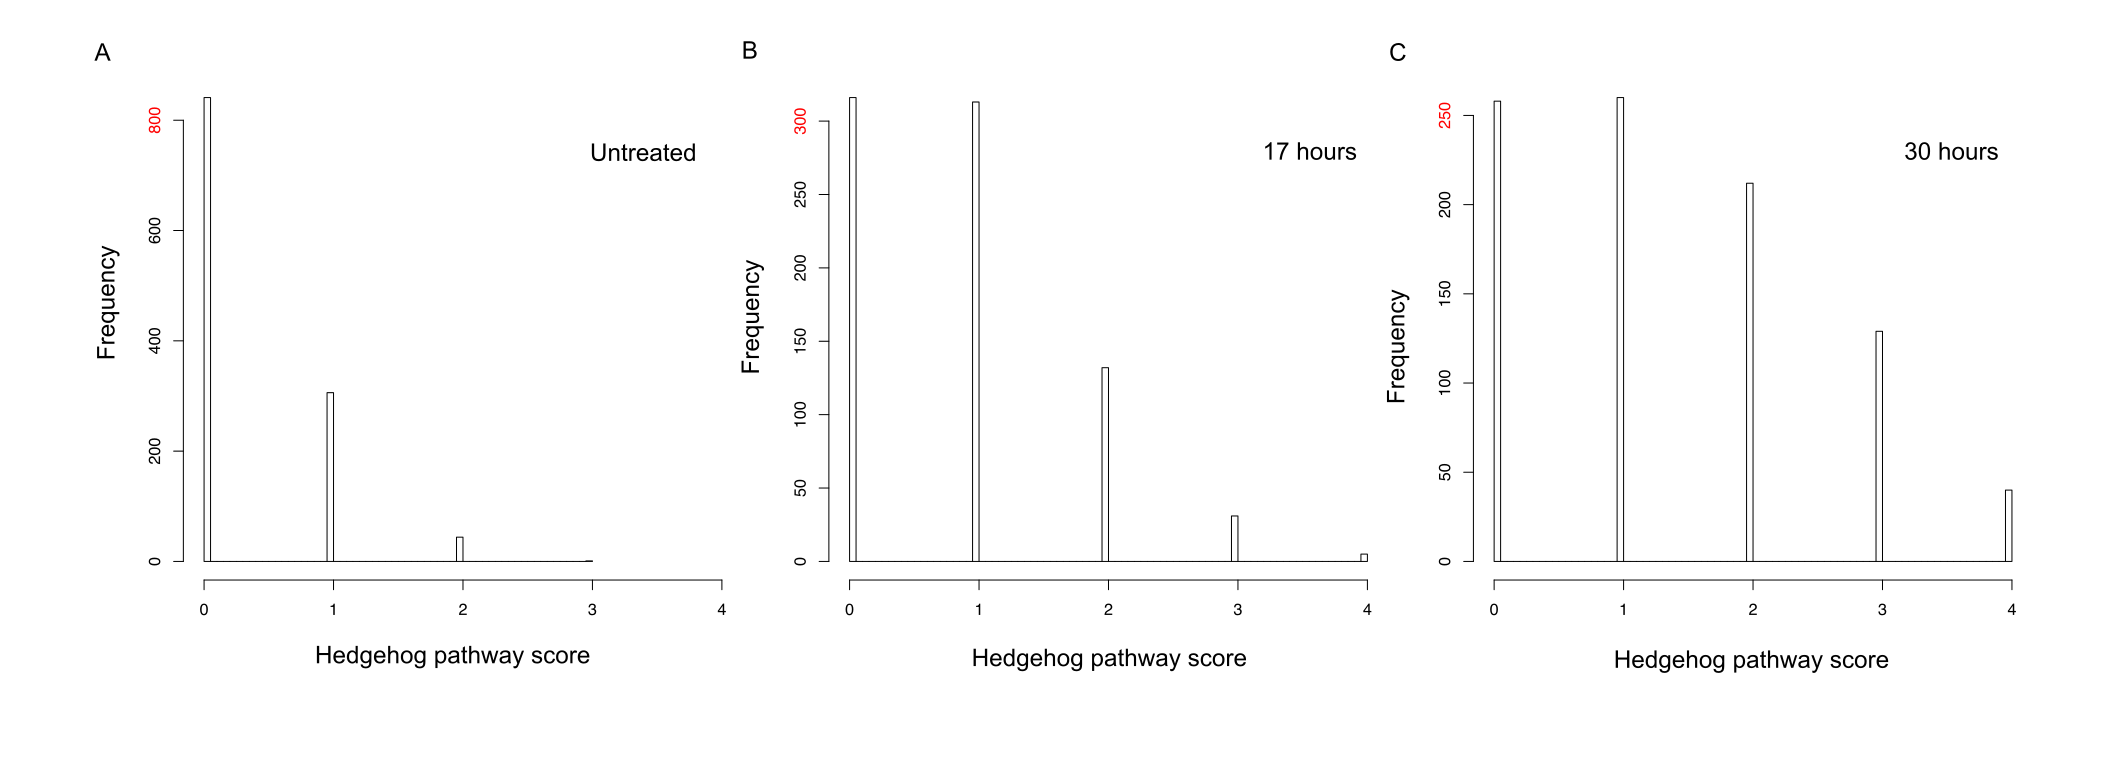
\includegraphics[width=\linewidth]{figures/hedgehog/SuppFigure7.png}
    \caption[Hedgehog score distribution at the 0, 17 and 30 hour time-points]{
        Hedgehog score distribution of cells at three different timepoints. For each cell, using the single-cell RNA sequencing data, we calculated the hedgehog score by looking at the expression of Gli1, Gli2, Ptch1 and GFP.  We assigned each gene in each cell a score of 1 if detected above background expression level, and we summed across the four genes to compute a score in the range [0-4]. In the untreated population scores are close to zero, by 30 hours more cells respond and the responders are the cells with score >= 3. Note the y-axis for each panel is different, however the interpretation is made by looking at the distribution of scores within each panel.  
    }
    \label{fig:hh_figureS7}
\end{suppfigure}


\begin{suppfigure}[p]  
    \centering
    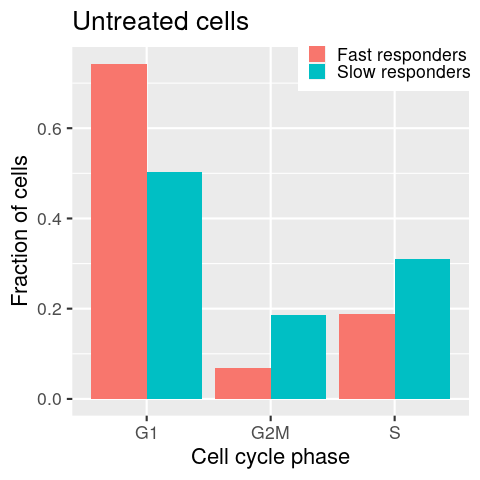
\includegraphics[width=\linewidth]{figures/hedgehog/SuppFigure8.png}
    \caption[Cell cycle assignments for fast responders and slow responders]{
        Inferred cell cycle phase for fast responders and slow responders. We inferred the cell cycle phase using the CellCycleScoring function in Seurat. 
    }
    \label{fig:hh_figureS8}
\end{suppfigure}


\begin{suppfigure}[p]  
    \centering
    \phantomlabel{fig:hh_figureS9A}
    \phantomlabel{fig:hh_figureS9B}
    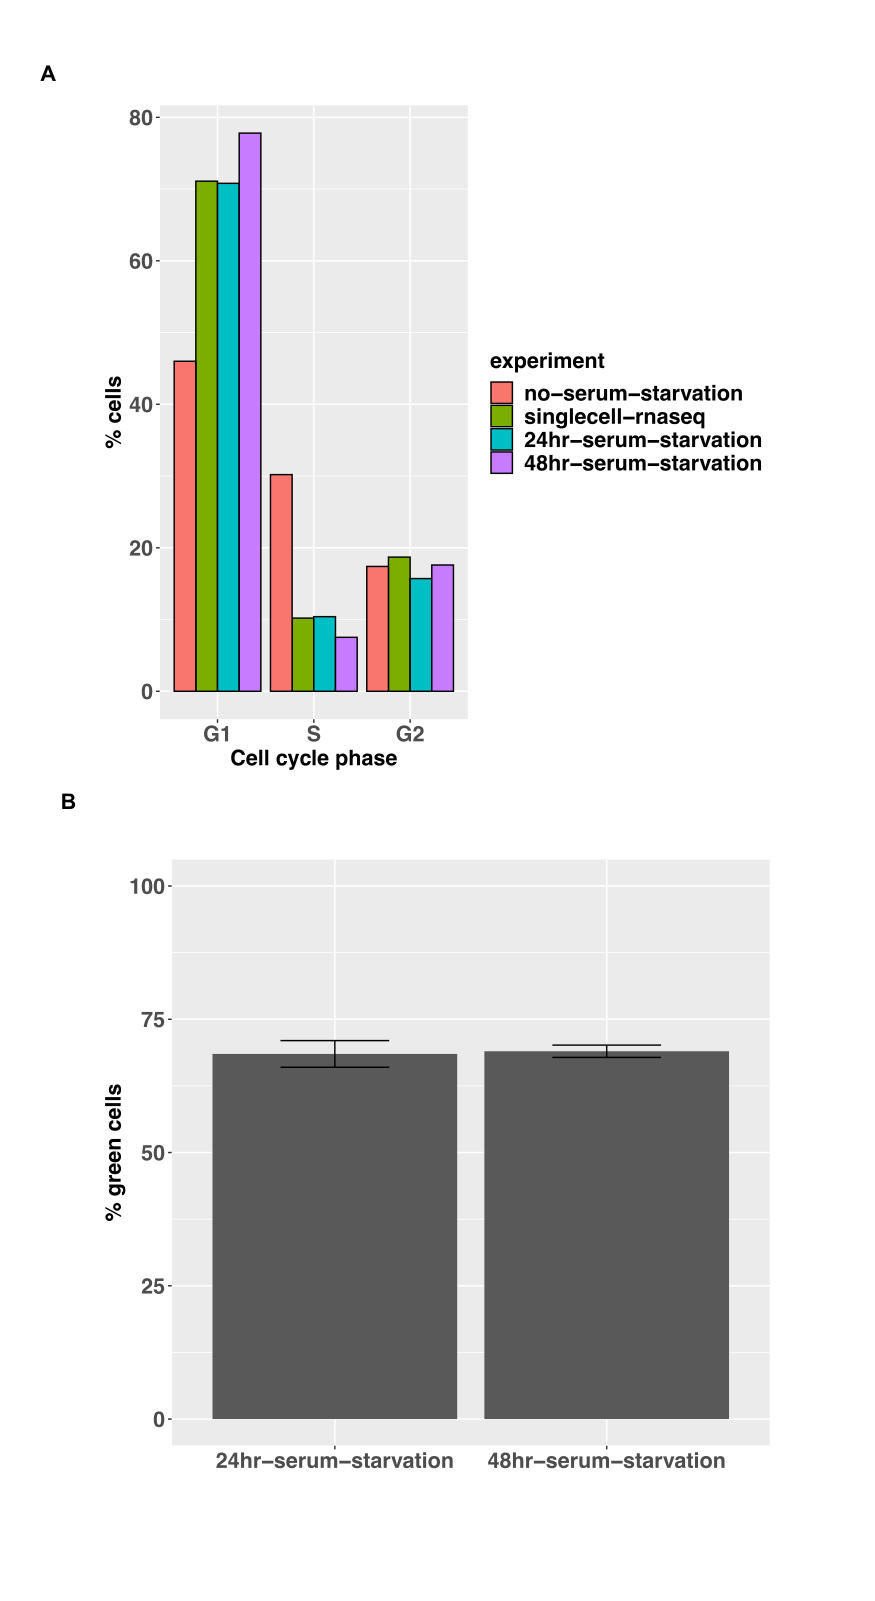
\includegraphics[width=\linewidth]{figures/hedgehog/SuppFigure9.png}
    \caption[No effect of serum starvation on response]{
        We used Propidium iodide staining to measure cell-cycle proportions of cells after 24 and 48 hours of serum starvation(using FlowJo CellCycle analysis), and compared to the cell cycle results for the untreated cells in \fref{fig:hh_figure1} estimated using Seurat (A) We serum-starved cells for 24 hours  (n = 2 replicates) and 48 hours (n = 3 replicates) performed the hedgehog assay as described on these two populations of cells and measured the fraction of responders after 30 hours using (B)
  
    }
    \label{fig:hh_figureS9}
\end{suppfigure}


\begin{suppfigure}[p]  
    \centering
    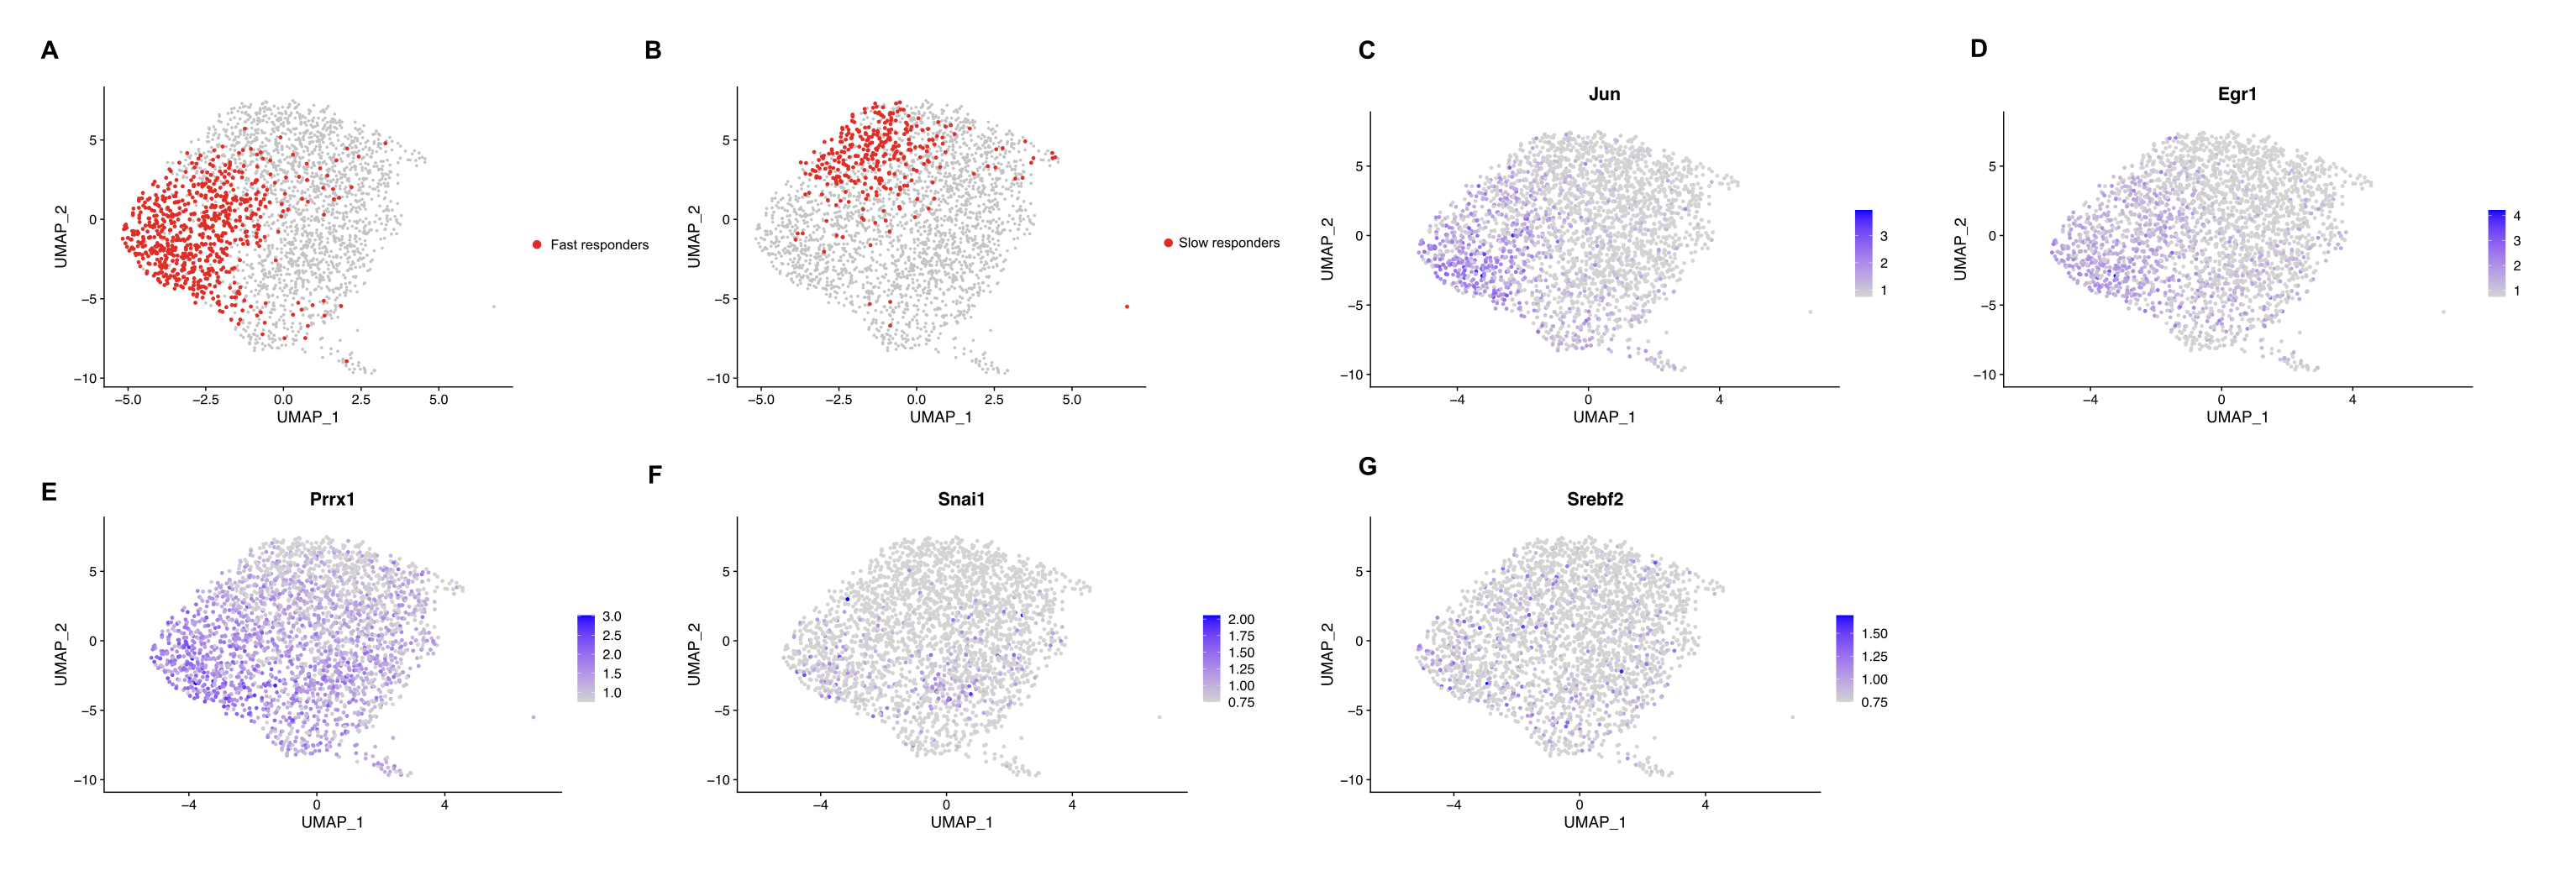
\includegraphics[width=\linewidth]{figures/hedgehog/SuppFigure10.png}
    \caption[TF expression on UMAP]{
        The fast responder population (A) and slow responder population (B) are shown on the UMAP plots. TFs that are overexpressed in the fast responders compared to the slow responders are shown, Jun (C), Egr1 (D), Prrx1 (E),  Snai1 (F). The regulator of the cholesterol biosynthesis pathway which is differentially active in the fast responding cells is shown in (G)  
    }
    \label{fig:hh_figureS10}
\end{suppfigure}


\begin{suppfigure}[p]  
    \centering
    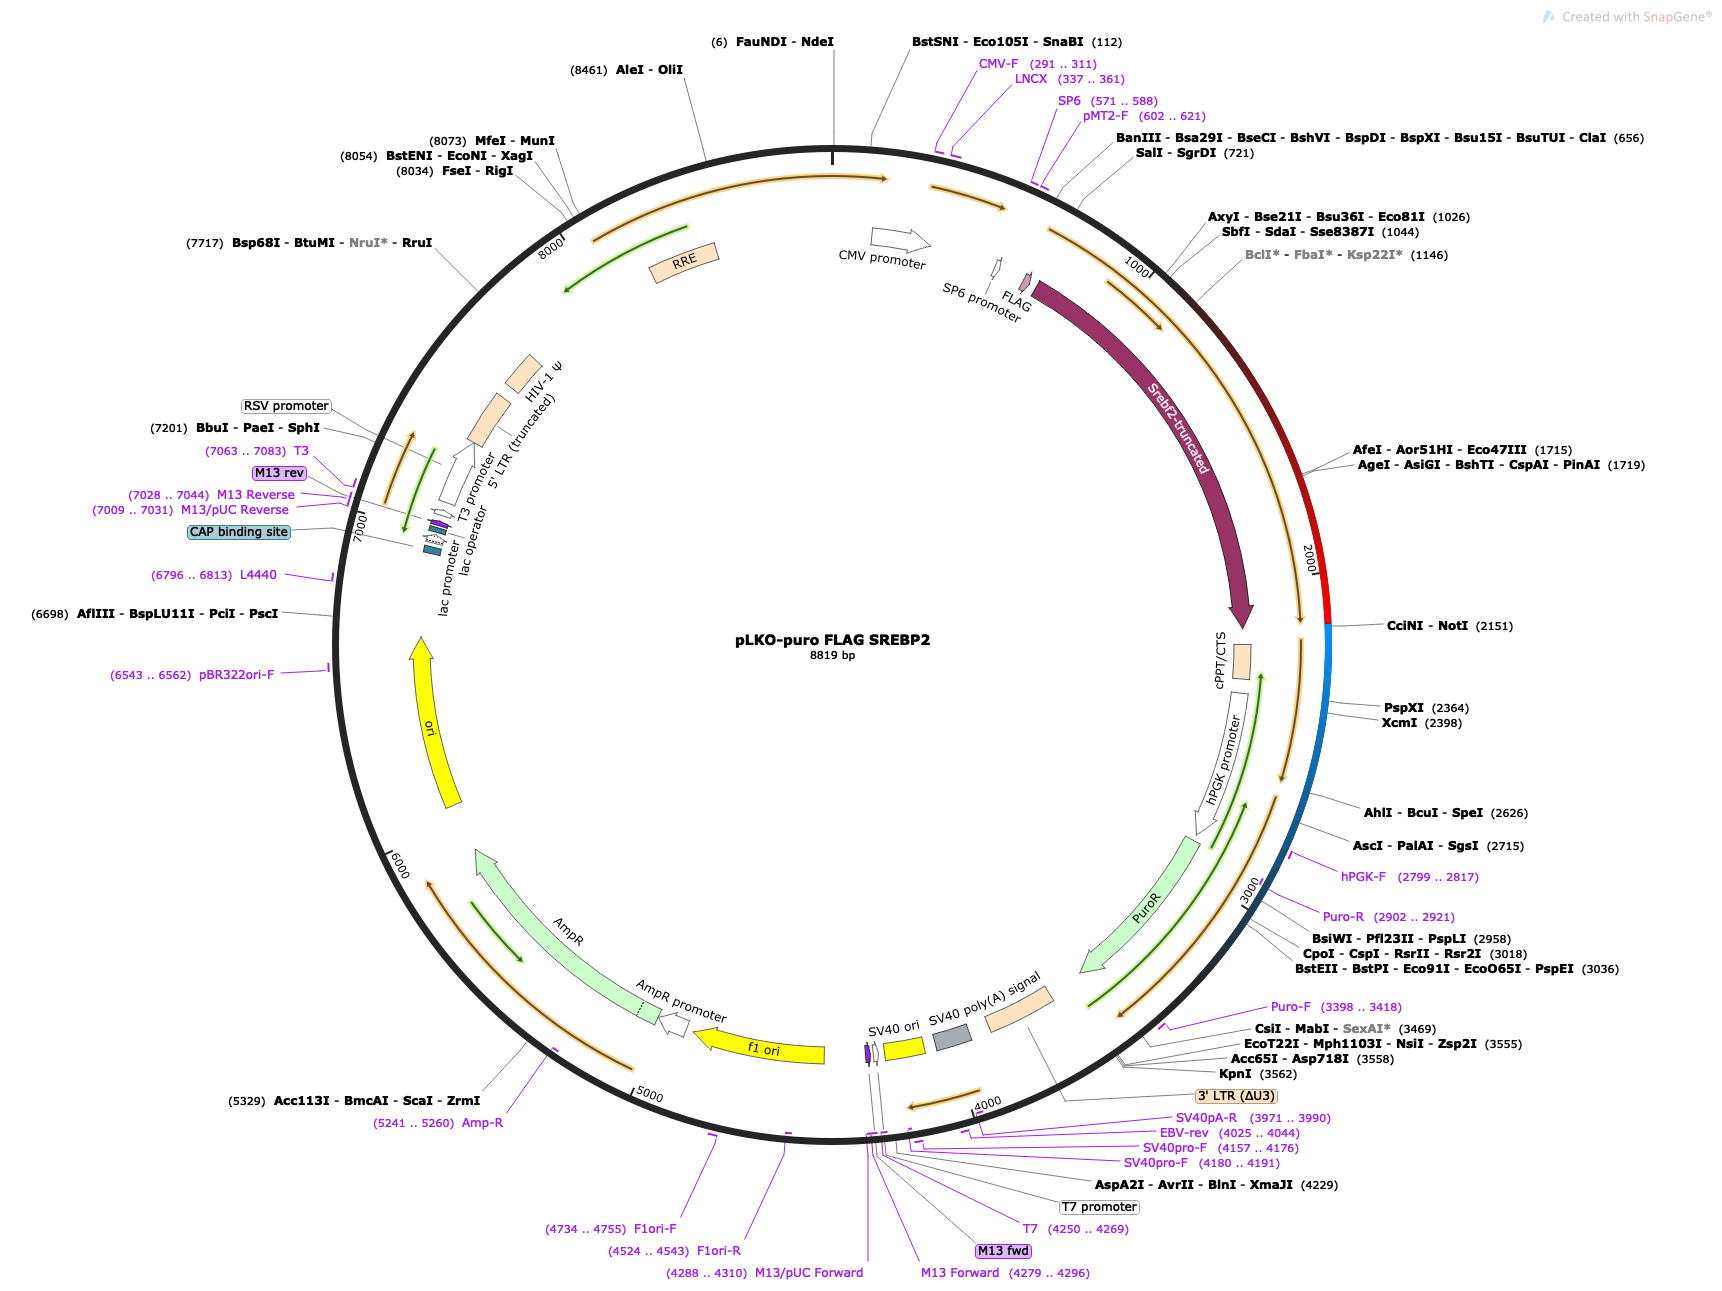
\includegraphics[width=\linewidth]{figures/hedgehog/SuppFigure11.png}
    \caption[Plasmid design for Srebf2 transfection]{
        Plasmid design for overexpressing Srebf2 via transfection. The coding region of truncated Srebf2 is under the control of the CMV promoter.
    }
    \label{fig:hh_figureS11}
\end{suppfigure}


\begin{suppfigure}[p]  
    \centering
    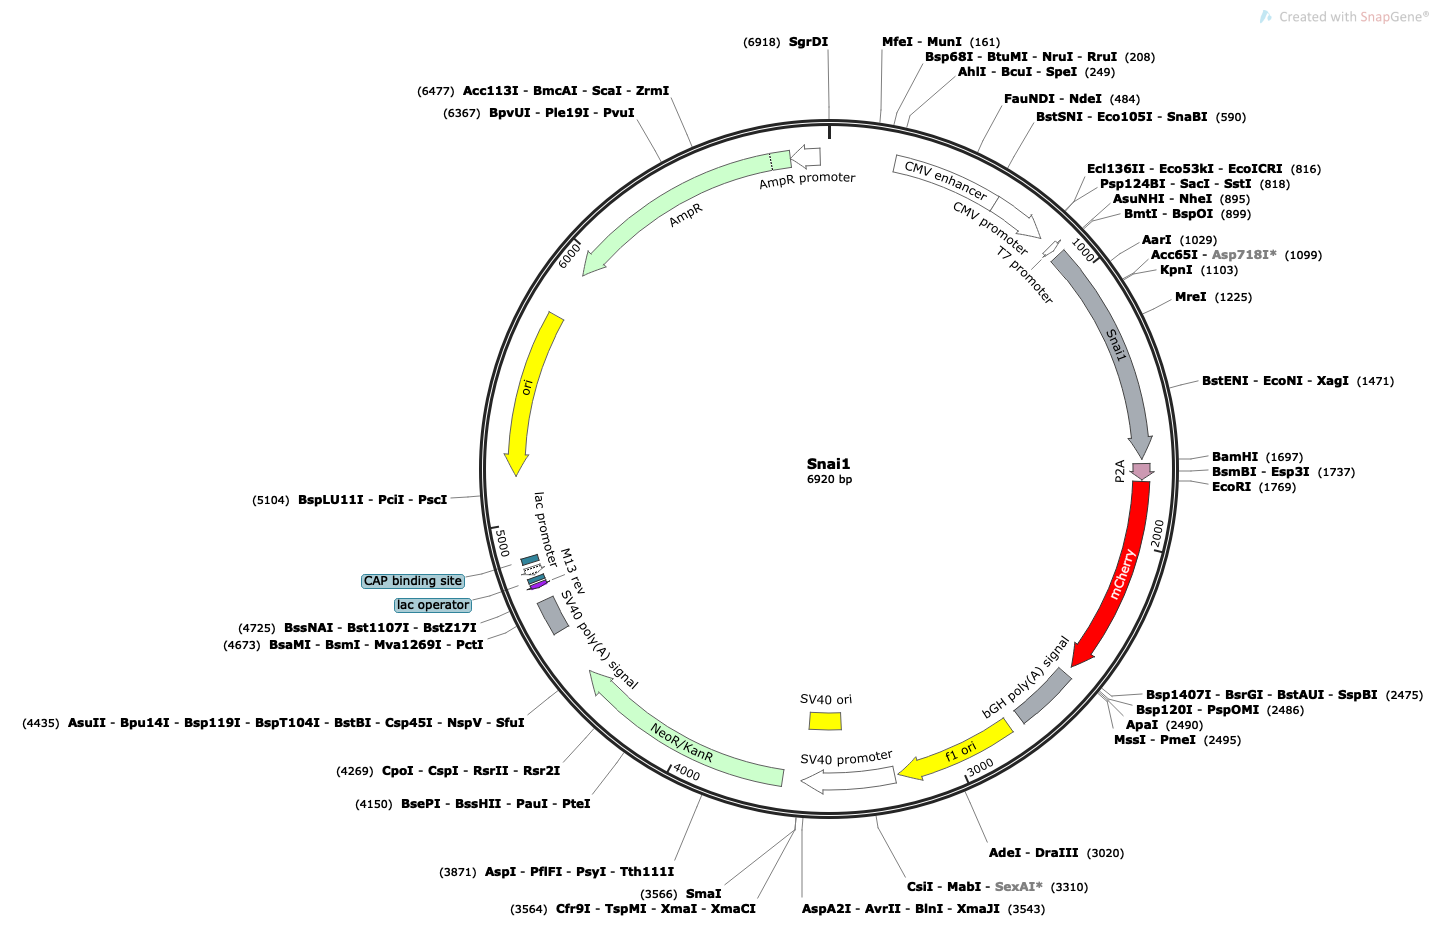
\includegraphics[width=\linewidth]{figures/hedgehog/SuppFigure12.png}
    \caption[Plasmid design for Snai1, Prrx1, Jun and Egr1 transfection]{
        Plasmid design for overexpressing Snai1. The coding region of Snai1 is regulated by the CMV promoter. This plasmid also contains a mCherry coding region to measure transfection efficiency on a cytometer. We used similarly designed plasmids for transfecting Jun, Egr1 and Prrx1 by replacing with the respective coding sequence.
  
    }
    \label{fig:hh_figureS12}
\end{suppfigure}


\begin{suppfigure}[p]  
    \centering
    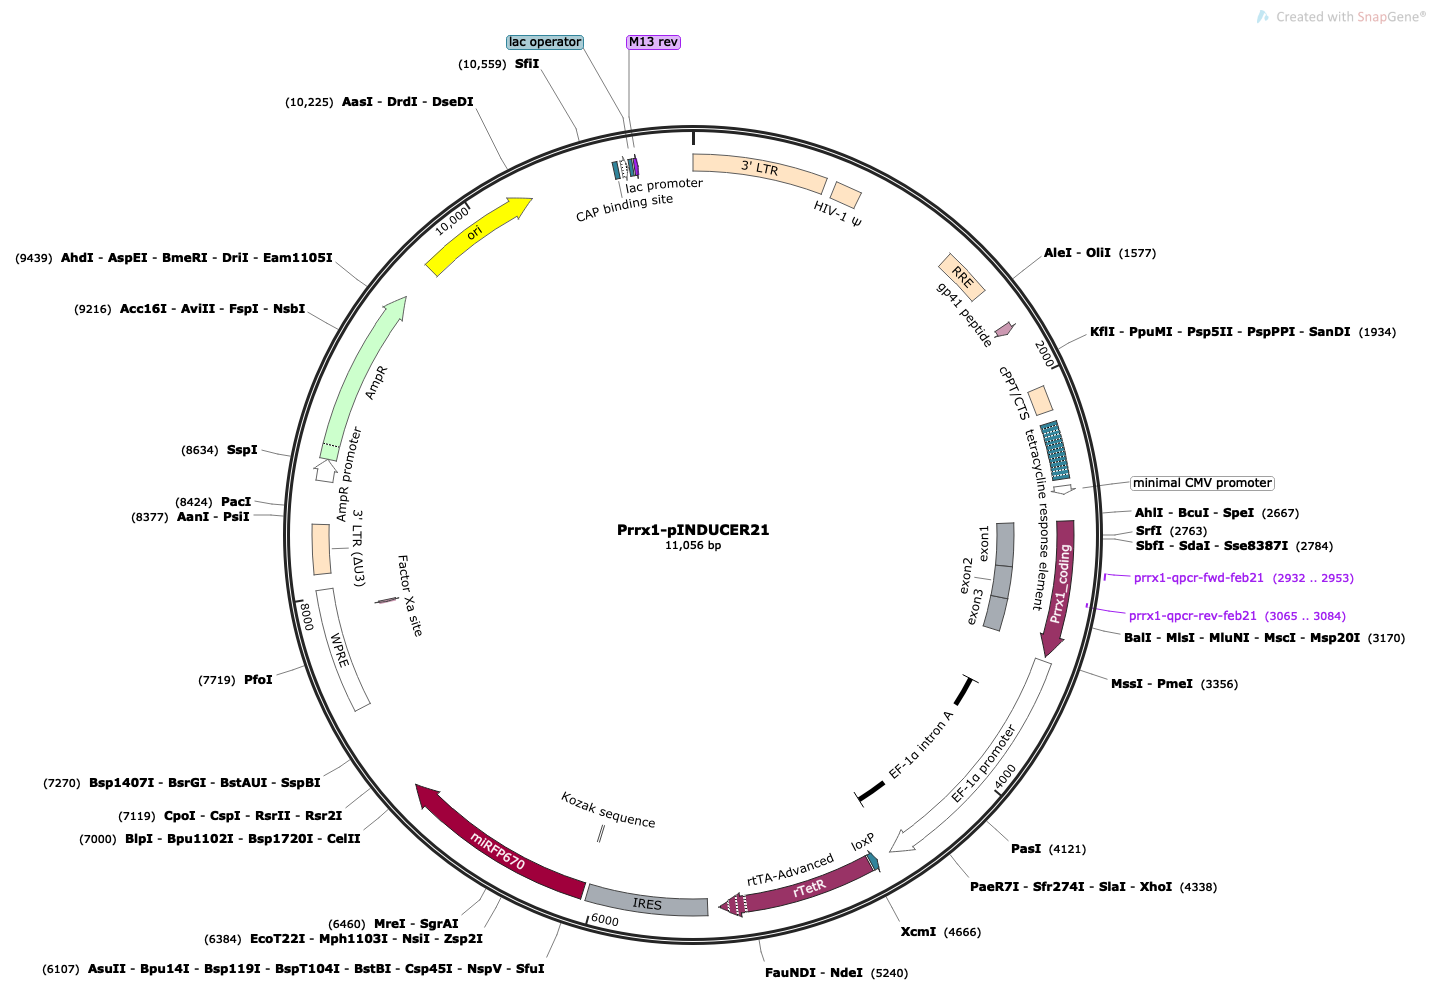
\includegraphics[width=\linewidth]{figures/hedgehog/SuppFigure13.png}
    \caption[Plasmid design for Snai1, Prrx1 lentiviral transduction]{
        Construct for Prrx1 pInducer induction. Lentiviruses were generated using this plasmid. We used the same design for Snai1 by replacing the coding region of Prrx1 with the coding region of Snai1.  
    }
    \label{fig:hh_figureS13}
\end{suppfigure}


\begin{suppfigure}[p]  
    \centering
    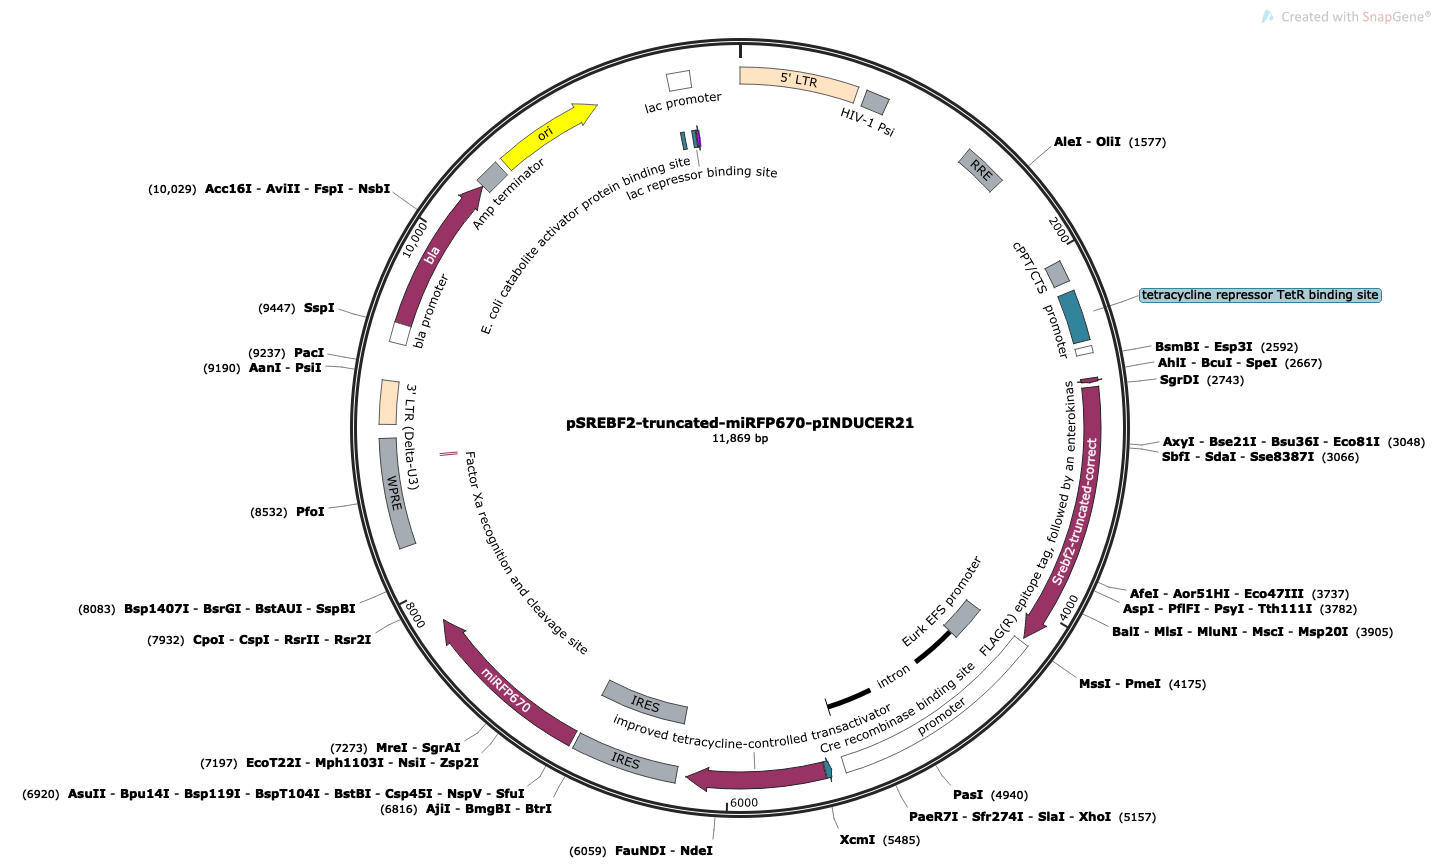
\includegraphics[width=\linewidth]{figures/hedgehog/SuppFigure14.png}
    \caption[Plasmid design for Srebf2 lentiviral transduction]{
        Construct for Srebf2 pInducer induction. Lentiviruses were generated using this plasmid.  
    }
    \label{fig:hh_figureS14}
\end{suppfigure}


\begin{suppfigure}[p]  
    \centering
    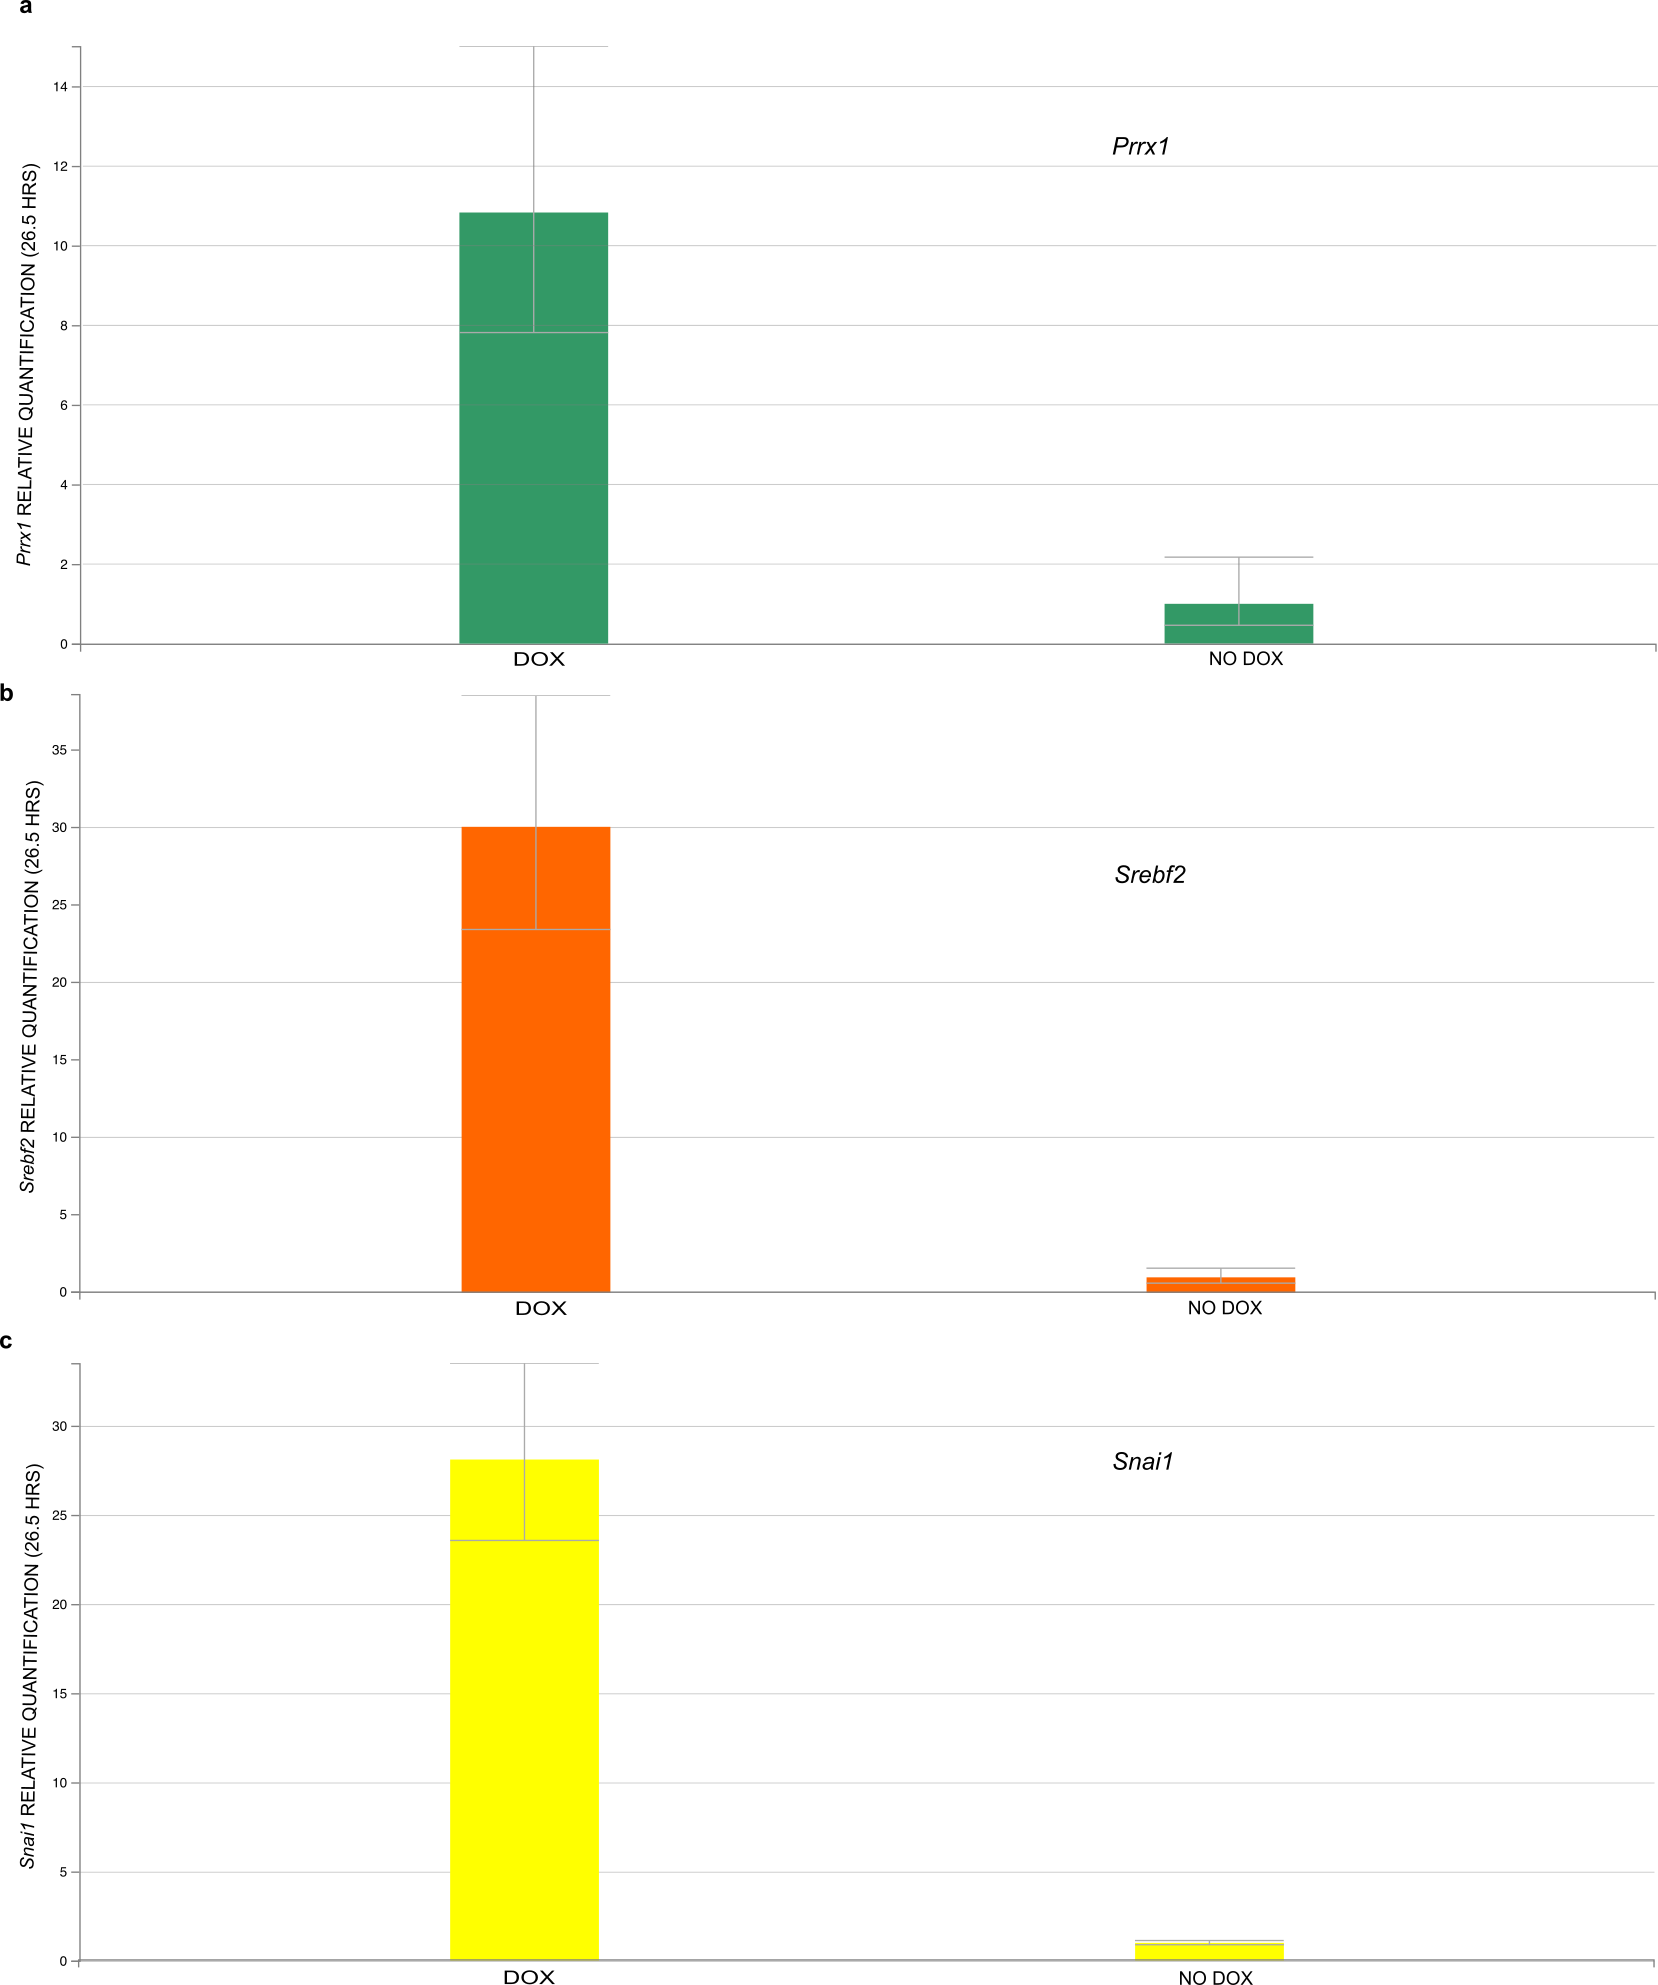
\includegraphics[width=\linewidth]{figures/hedgehog/SuppFigure15.png}
    \caption[qPCR induction plots for Prrx1, Srebf2 and Snai1]{
        Induction of Prrx1, Srebf2 and Snai1. Cell lines with inducible Prrx1(a), Srebf2 (b) and Snai1 (c) were treated with Doxycycline to induce the expression of the three genes. After 26.5 hours, we harvested the cells and used the RNA for qPCR assays. We used cells with no Doxycycline added as controls. We compared RNA levels in each condition to the housekeeping control gene Hprt.  
    }
    \label{fig:hh_figureS15}
\end{suppfigure}



\begin{suppfigure}[p]  
    \centering
    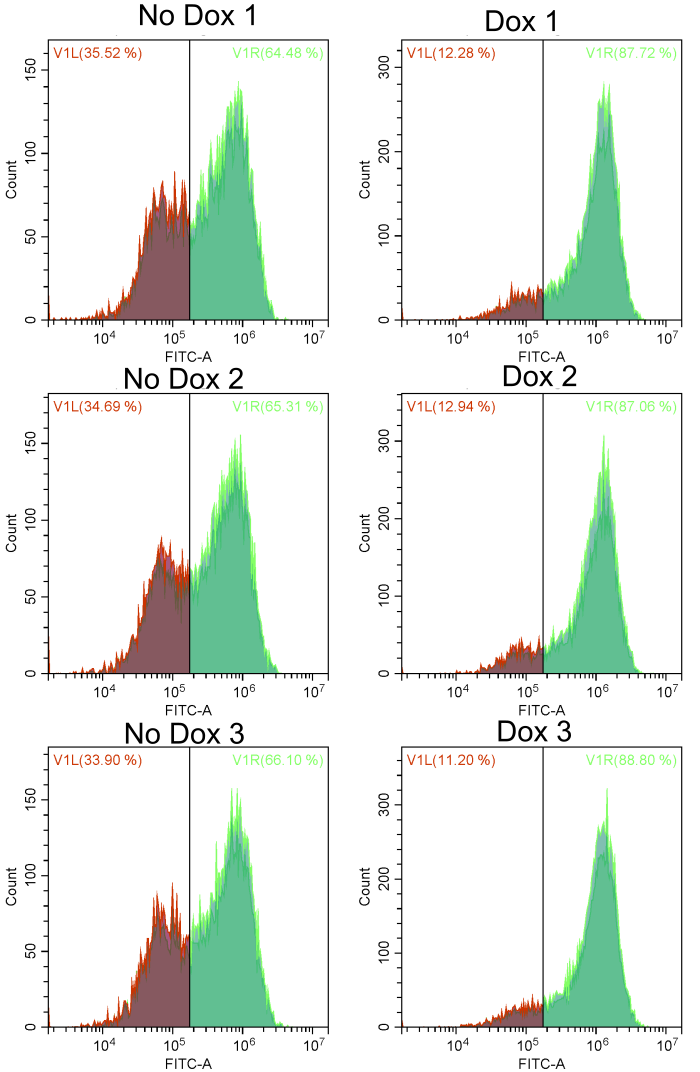
\includegraphics[width=\linewidth]{figures/hedgehog/SuppFigure16.png}
    \caption[Raw data for the Prrx1 induced and uninduced cells shown in \fref{fig:hh_figure3a}]{
        Raw cytometer plots for the data summarized in \fref{fig:hh_figure3a}. Prrx1 inducible cells were grown in the presence and absence of Dox, treated with SAG and run on a cytometer at 32 hours. Three biological replicates were used for each condition.  
    }
    \label{fig:hh_figureS16}
\end{suppfigure}


\begin{suppfigure}[p]  
    \centering
    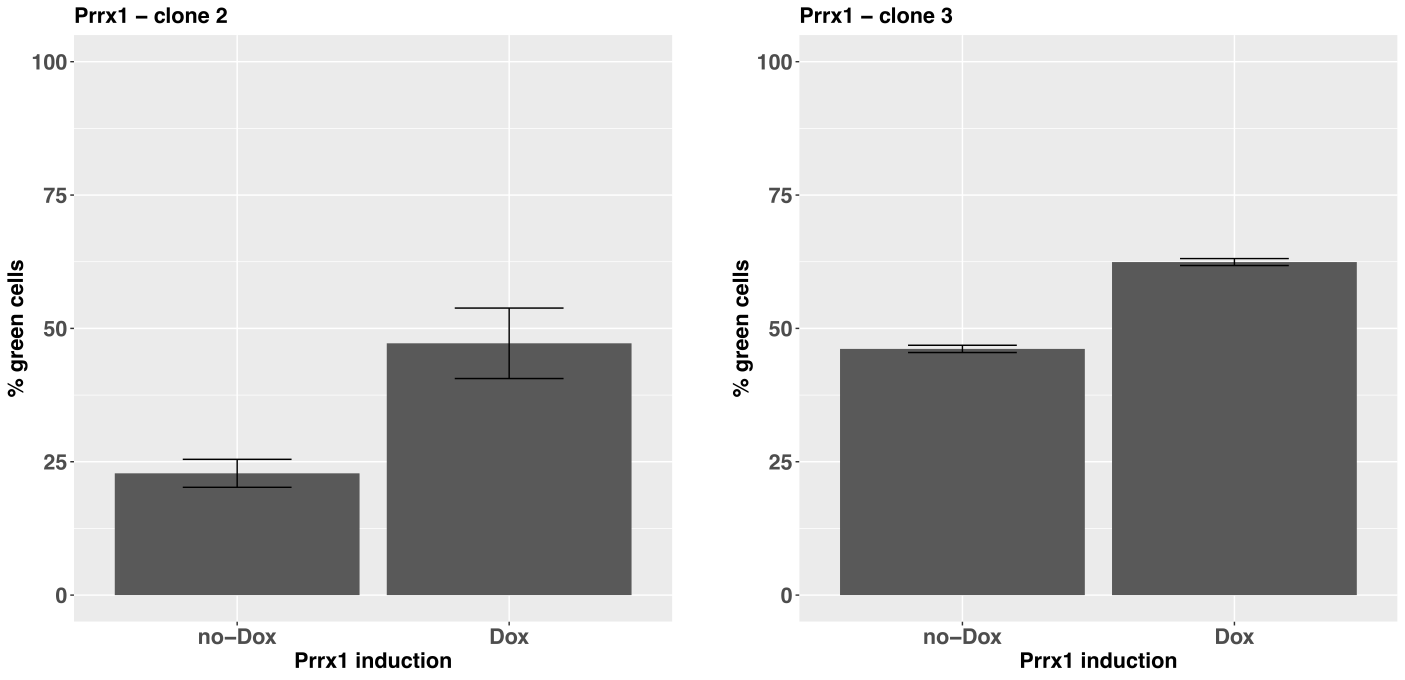
\includegraphics[width=\linewidth]{figures/hedgehog/SuppFigure17.png}
    \caption[No difference in percent green for Prrx1 induction followed by SAG treatment - Clones 2, 3]{
        Additional clones showing difference in response after Prrx1 induction. Shown are the mean percentage responders (in red) +/- standard error of the mean.  
    }
    \label{fig:hh_figureS17}
\end{suppfigure}


\begin{suppfigure}[p]  
    \centering
    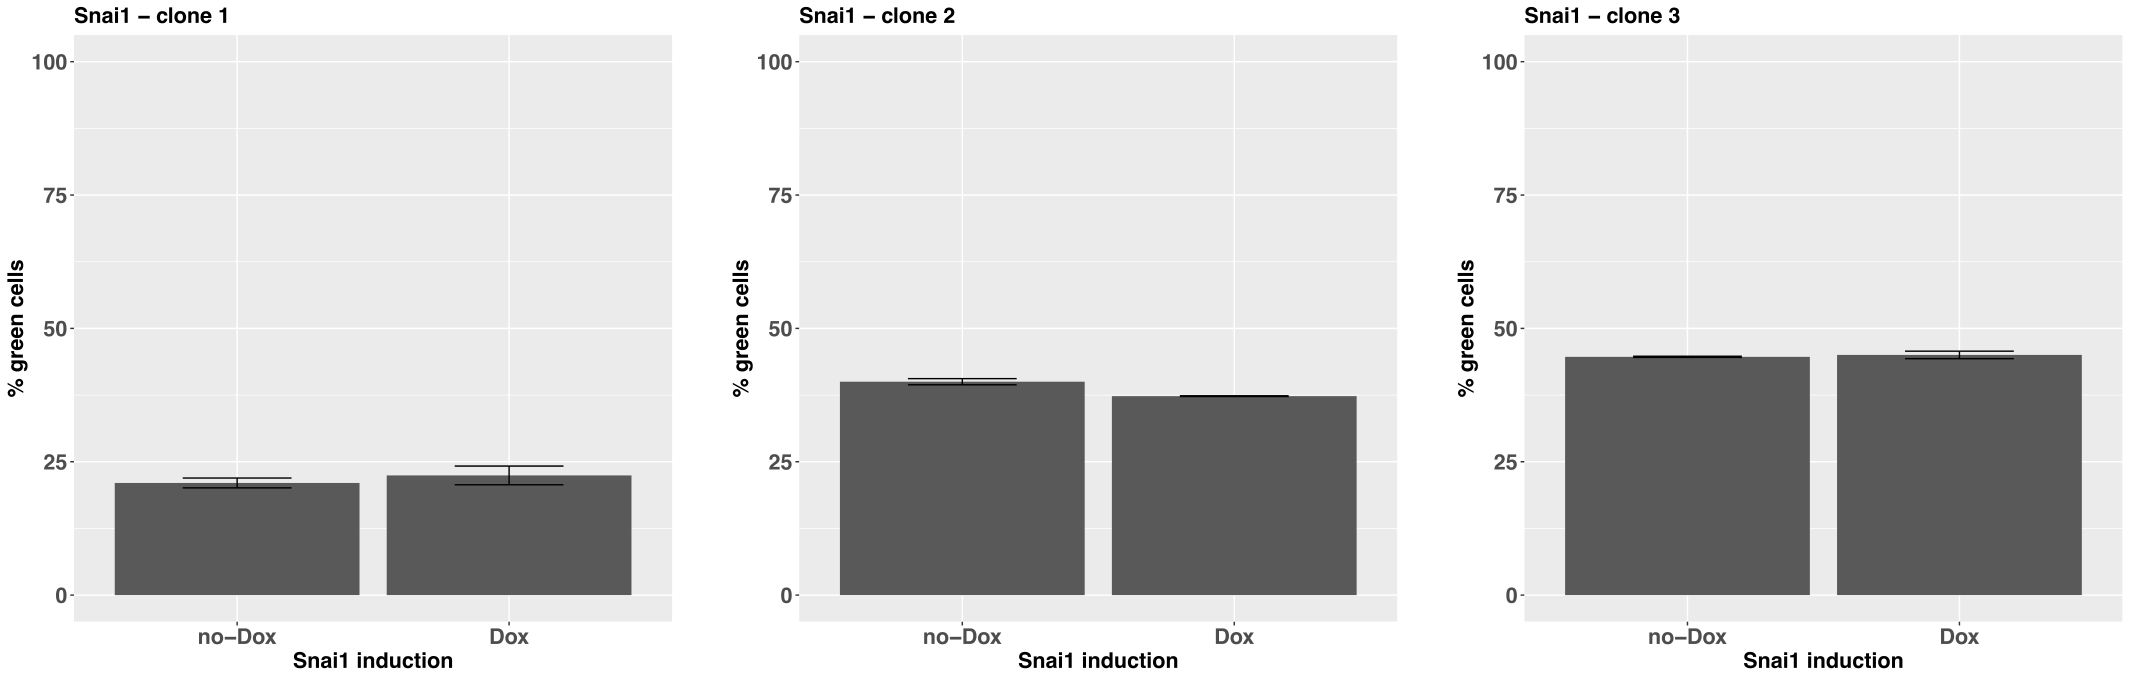
\includegraphics[width=\linewidth]{figures/hedgehog/SuppFigure18.png}
    \caption[No difference in percent green for Snai1 induction followed by SAG treatment]{
        No difference in hedgehog assay response after Snai1 induction. We grew cells integrated with inducible Snai1 in the presence and absence of Doxycycline. We performed the Hedgehog assay on the two groups (three replicates each) of cells by adding SAG and observing the percent of cells that respond on the flow cytometer after 32 hours. We did this for three separate clones after transduction. Shown are the mean percentage of responders (in red) +/- standard error of the mean.
    }
    \label{fig:hh_figureS18}
\end{suppfigure}


\begin{suppfigure}[p]  
    \centering
    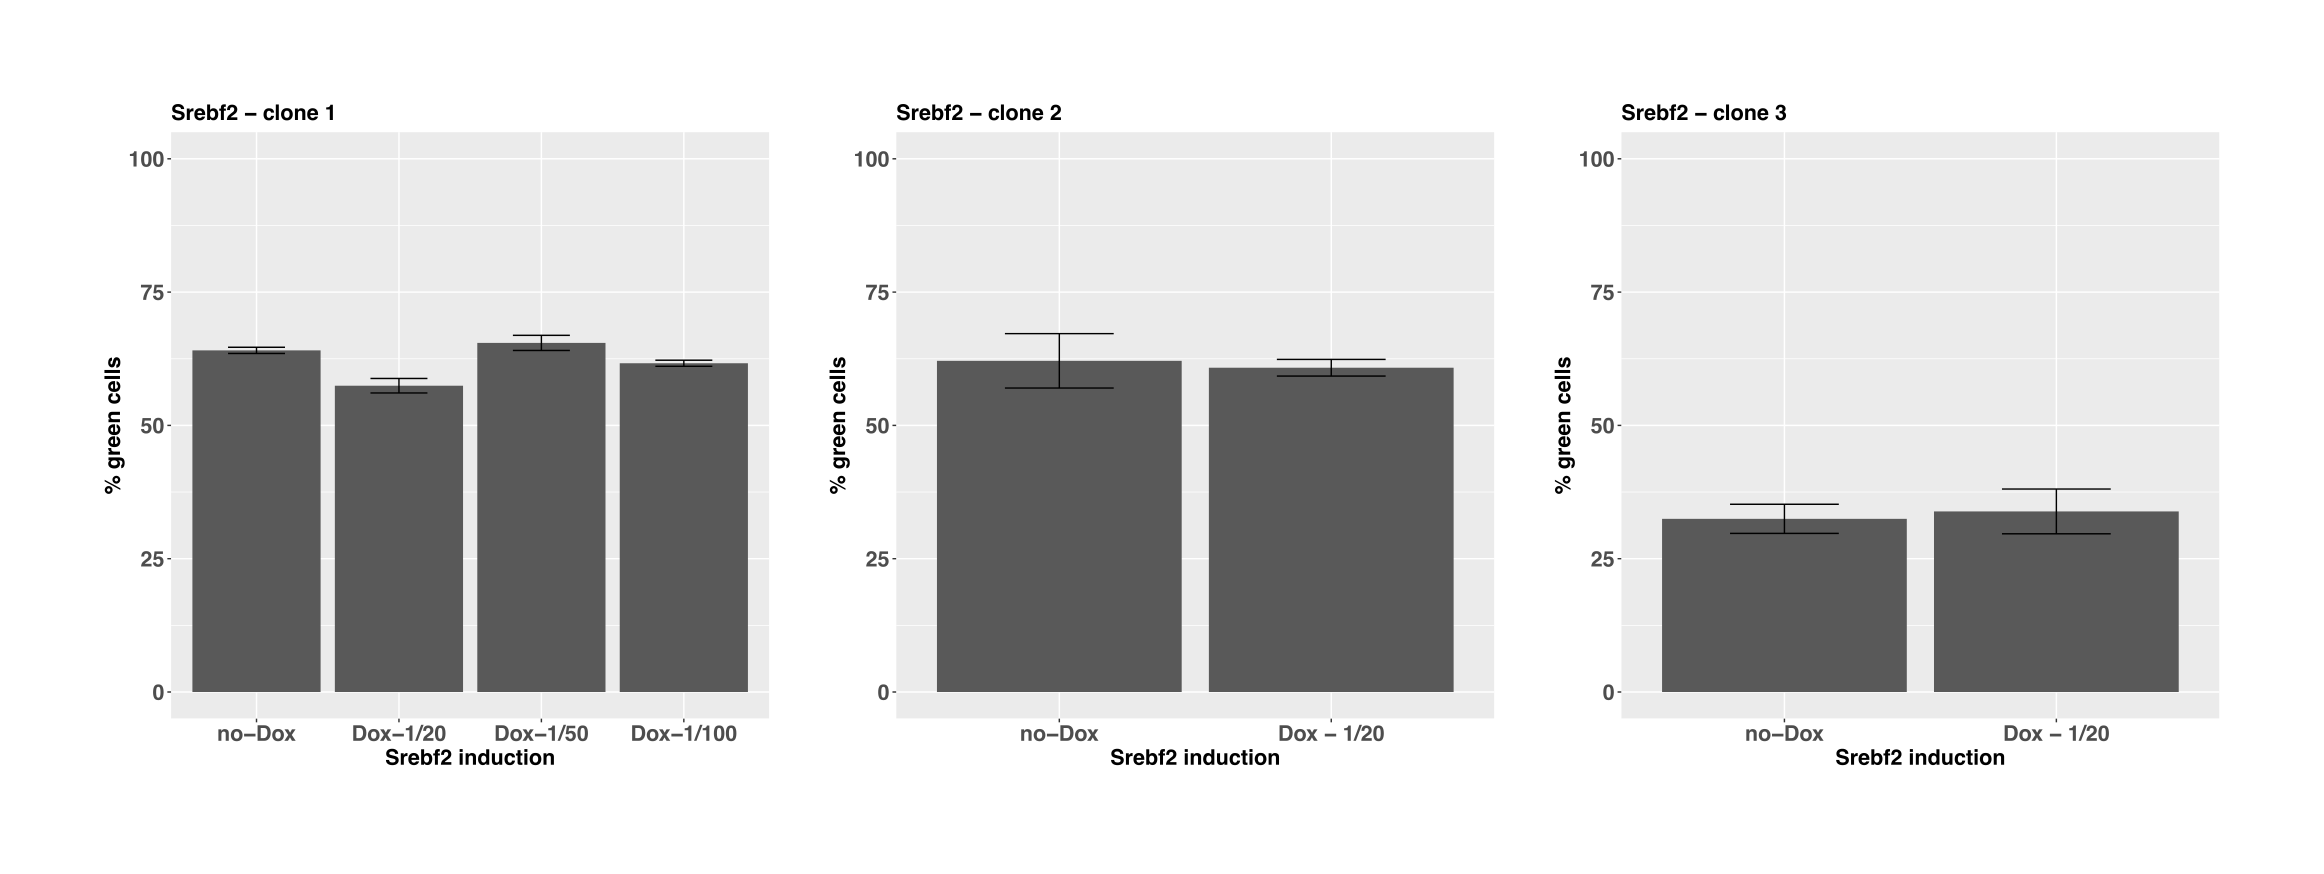
\includegraphics[width=\linewidth]{figures/hedgehog/SuppFigure19.png}
    \caption[No difference in percent green for Srebf2 induction followed by SAG treatment]{
        No difference  in hedgehog assay response after Srebf2 induction. We grew cells integrated with inducible Srebf2 in the presence and absence of Doxycycline. We used three different concentrations of Dox. Cells did not survive in the presence of 1X and 0.1X Dox. In this figure, 1X Dox is the same concentration of Dox used for Prrx1 and Snai1 (500 ng/ml). We performed the hedgehog assay on the two groups (three technical replicates each) of cells by adding SAG and observing the percent of cells that respond on the flow cytometer after 46 hours. We did this for three separate clones after transduction.  Shown are the mean percentage responders (in red) +/- standard error of the mean.  
    }
    \label{fig:hh_figureS19}
\end{suppfigure}


\begin{suppfigure}[p]  
    \centering
    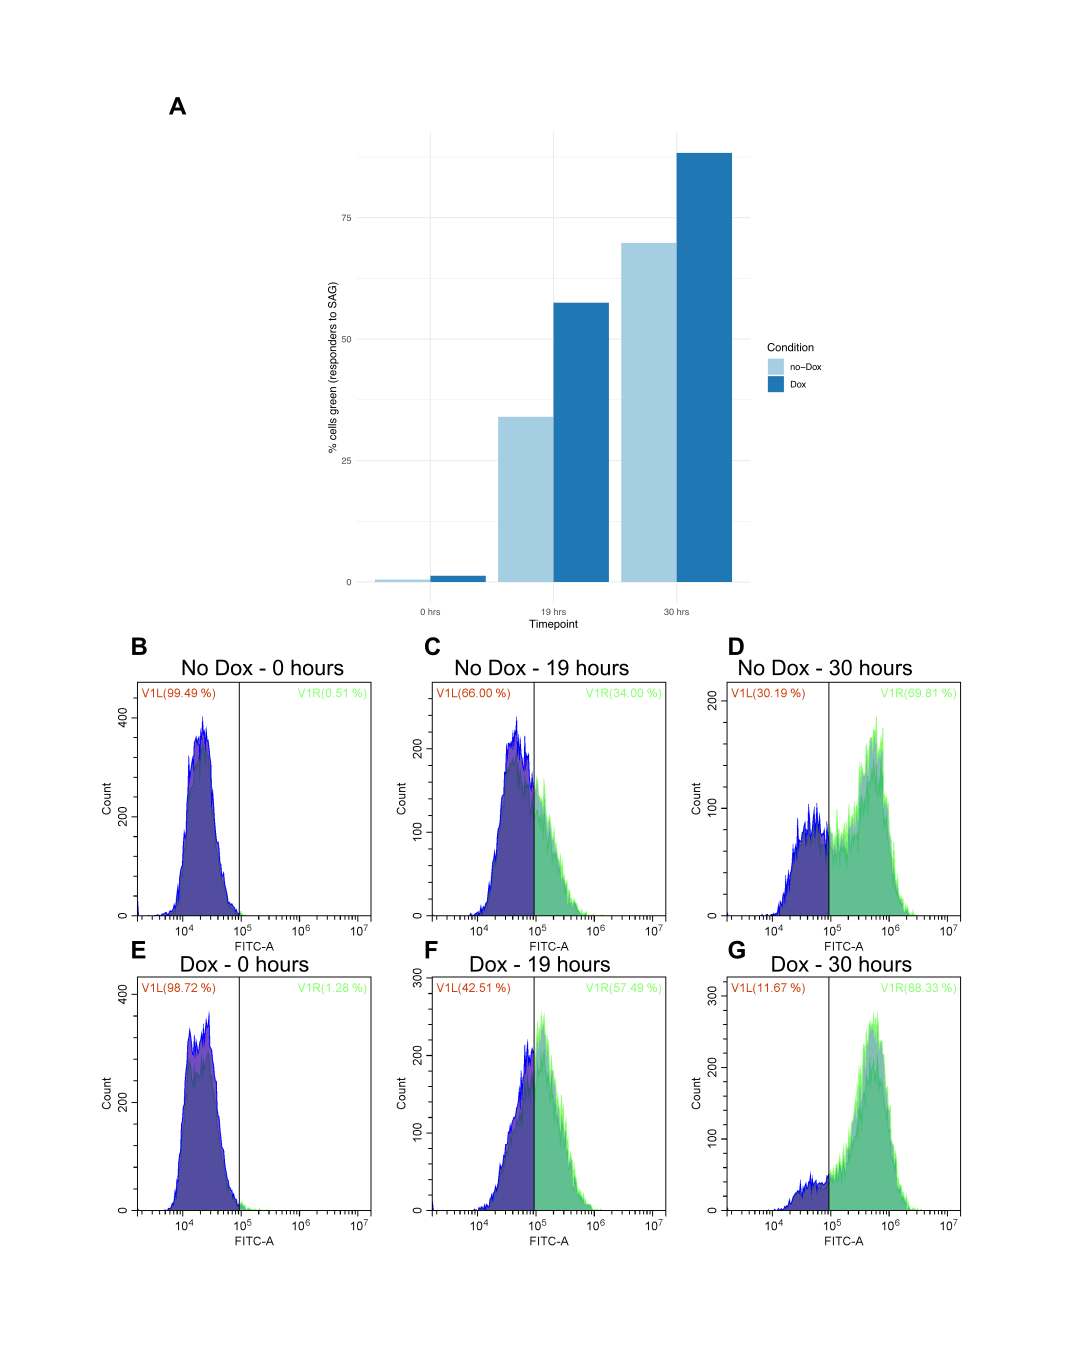
\includegraphics[width=\linewidth]{figures/hedgehog/SuppFigure20.png}
    \caption[Flow Cytometry results for cells used in Prrx1 induction single-cell RNA sequencing experiment]{
        Response of Prrx1 induced and induced cells from the same pool as the cells used for the single-cell RNA sequencing experiments in \fref{fig:hh_figure4} (A) Percentage responding cells(GFP fluorescence) on a cytometer summarized  at 0 (untreated), 19 and 30 hours. (B), (C ), (D)Raw cytometer plots for the same cells in (A) in the no Dox condition. (E), (F), (G) Raw cytometer plots for the same cells in (A) grown in the Dox condition. This figure show one replicate at each condition used in the single-cell RNA sequencing experiment, biological replicates of Prrx1-induction response result is shown in \fref{fig:hh_figure3} and \fref{fig:hh_figureS13}. 
    }
    \label{fig:hh_figureS20}
\end{suppfigure}


\begin{suppfigure}[p]  
    \centering
    \phantomlabel{fig:hh_figureS21A}
    \phantomlabel{fig:hh_figureS21B}
    \phantomlabel{fig:hh_figureS21C}
    \phantomlabel{fig:hh_figureS21D}
    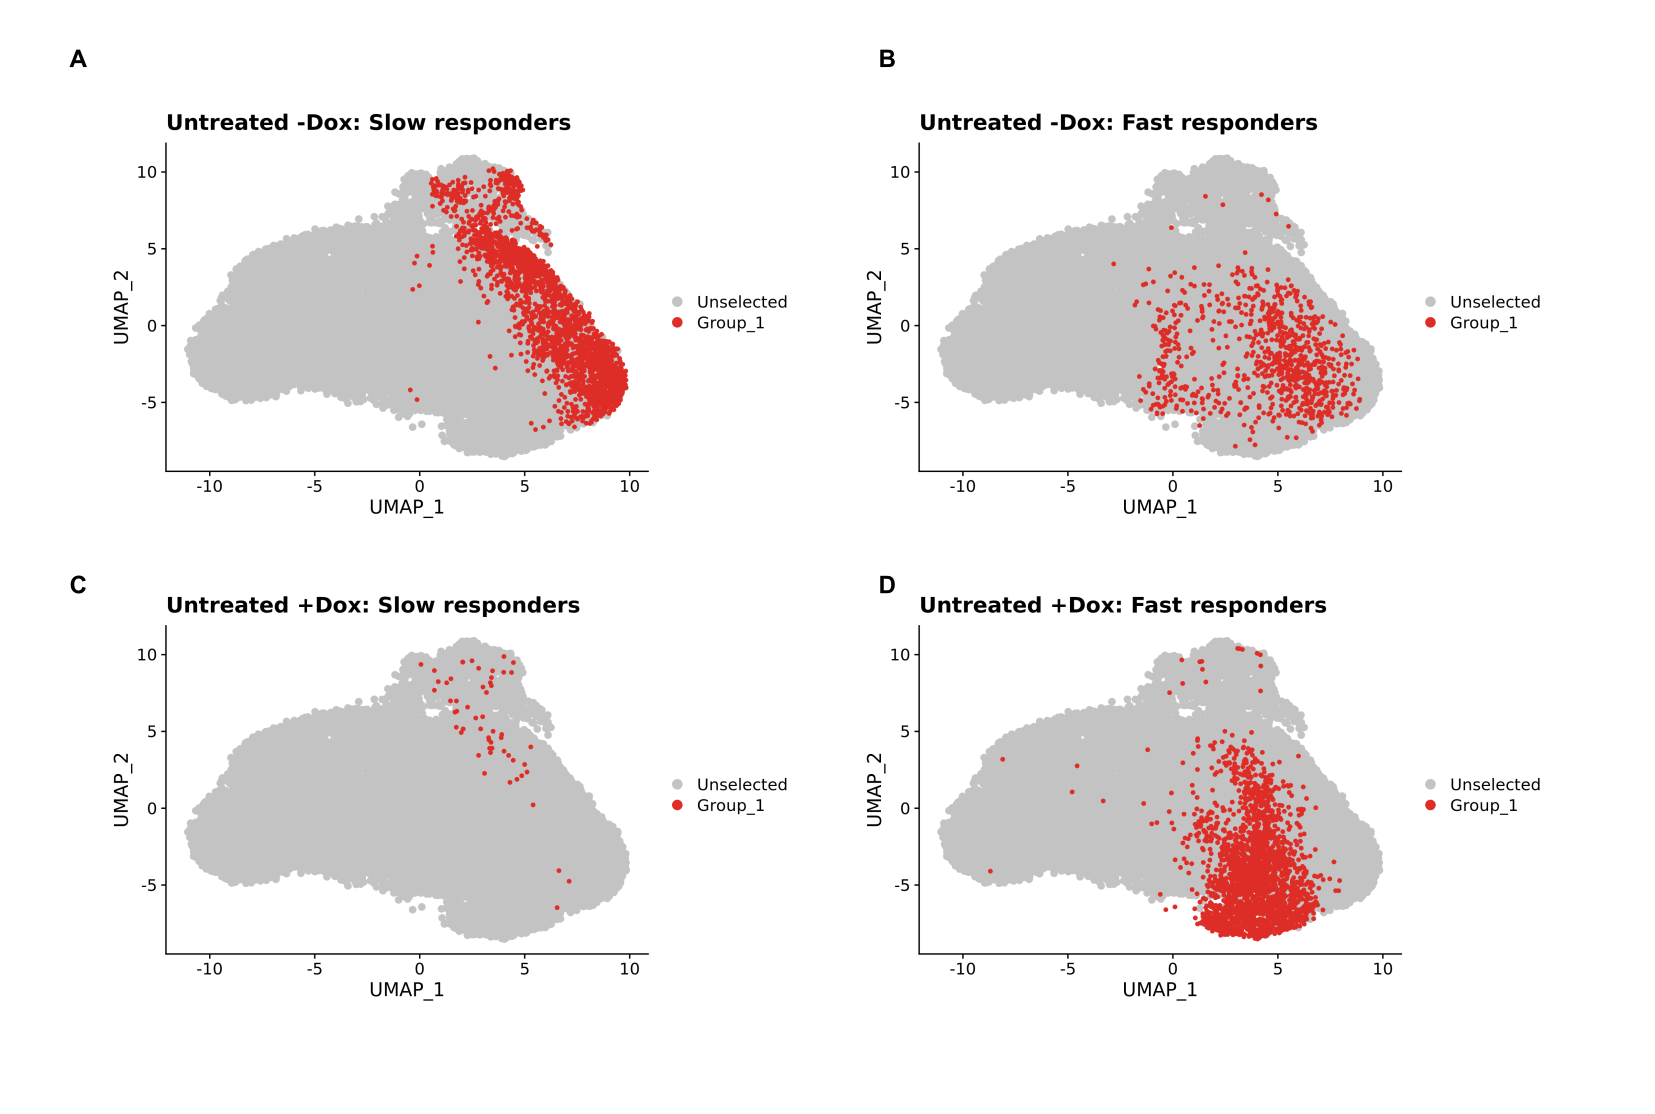
\includegraphics[width=\linewidth]{figures/hedgehog/SuppFigure21.png}
    \caption[Predicted slow and fast responder cells using Garnett in the Prrx1 +/- Dox untreated cells]{
        Predicted fast and slow responders from Garnett.
        We trained a cell-type classifier on the fast and slow responder cells in \fref{fig:hh_figure1} to learn the features of fast and slow responders. We next applied this trained classifier on untreated (0 hours) cells with inducible Prrx1, used in \fref{fig:hh_figure4}, to identify the fast and slow responders in this population. (A) and (B) show the slow and fast responders identified by the model in the untreated cells grown in the absence of Dox. In the cells grown in the absence of Dox, the classifier identifies a mixture of slow and fast responders. © and (D) show the slow and fast responders identified by the model in the untreated cells grown in the presence of Dox. In the cells grown in the presence of Dox, most of the cells are classified as fast reponders by the classifier.
    }
    \label{fig:hh_figureS21}
\end{suppfigure}


\chapter{Effect of genomic and cellular environments on gene expression noise}
\label{chap:cas}

This work was performed in collaboration in with Clarice Hong, Siqi Zhao and Barak Cohen. All authors conceived and designed the project. I performed 10X sample preparation and library preparation, co-developed a pipeline to go from the raw reads to UMI counts for each location in each cell, performed the modeling of mean and noise as a function of covariates. Clarice Hong, Siqi Zhao and I are co-first authors on this manuscript that all authors wrote together. The manuscript is currently under review and has been uploaded to \textit{Biorxiv} (doi: \href{https://www.biorxiv.org/content/10.1101/2022.08.31.506082v1}{10.1101/2022.08.31.506082}) \cite{hongcky_cohenba:EffectGenomic2022}.

\section{Abstract}

Individual cells from isogenic populations often display large cell-to-cell differences in gene expression. This \enquote{noise} in expression derives from several sources, including the genomic and cellular environment in which a gene resides. Large-scale maps of genomic environments have revealed the effects of epigenetic modifications and transcription factor occupancy on mean expression levels, but leveraging such maps to explain expression noise will require new methods to assay how expression noise changes at locations across the genome. To address this gap, we present \underline{S}ingle-cell \underline{A}nalysis of \underline{R}eporter \underline{G}ene \underline{E}xpression \underline{N}oise and \underline{T}ranscriptome (SARGENT), a method that simultaneously measures the noisiness of reporter genes integrated throughout the genome and the global mRNA profiles of individual reporter-gene-containing cells. Using SARGENT, we performed the first comprehensive genome-wide survey of how genomic locations impact gene expression noise. We found that the mean and noise of expression correlate with different histone modifications. We quantified the intrinsic and extrinsic components of reporter gene noise and, using the associated mRNA profiles, assigned the extrinsic component to differences between the CD24+ \enquote{stem-like} sub-state and the more \enquote{differentiated} sub-state. SARGENT also reveals the effects of transgene integrations on endogenous gene expression, which will help guide the search for \enquote{safe-harbor} loci. Taken together, we show that SARGENT is a powerful tool to measure both the mean and noise of gene expression at locations across the genome, and that the data generated by SARGENT reveals important insights into the regulation of gene expression noise genome-wide. 

\section{Introduction}

Gene expression is noisy, even among individual cells from an isogenic population \cite{raja_vanoudenaardena:NatureNurture2008}. Noisy gene expression leads to variable cellular outcomes in differentiation \cite{changhh_huangs:TranscriptomewideNoise2008,kalmart_ariasam:RegulatedFluctuations2009,abranchese_henriqued:StochasticNANOG2014,desairv_weinbergerls:DNARepair2021}, the response to environmental stimuli \cite{spencersl_sorgerpk:NongeneticOrigins2009, topolewskip_komorowskim:PhenotypicVariability2022}, viral latency \cite{weinbergerls_schafferdv:StochasticGene2005}, and chemotherapeutic drug resistance \cite{shaffersm_raja:RareCell2017, emertbl_raja:VariabilityRare2021, yangc_spencersl:MelanomaSubpopulations2021}. Explaining the causes of noisy expression remains an important challenge. 

A gene’s genomic environment, defined here as the composition of nearby cis-regulatory elements and local epigenetic marks, can influence its expression noise. Some features of genomic environments that can affect noise include enhancers, histone modifications, and transcription factor (TF) occupancy \cite{wus_qianw:IndependentRegulation2017, darrd_weinbergerls:TranscriptionalBurst2012, larsondr_singerrh:DirectObservation2013, senecala_darzacqx:TranscriptionFactors2014, waltersmc_martindi:EnhancersIncrease1995, weinbergerl_barkain:ExpressionNoise2012,faureaj_lehnerb:SystematicAnalysis2017}. These observations raise the possibility that genome-wide patterns of expression noise could be explained using the large-scale epigenetic maps that have proved useful in explaining mean expression levels \cite{akhtarw_vansteenselb:ChromatinPosition2013,kundajea_kellism:IntegrativeAnalysis2015,karlicr_vingronm:HistoneModification2010}. Leveraging these resources to explain expression noise will require maps of the genome that show the influence of diverse genomic environments on this noise. Producing these maps will require new experimental approaches, because the existing studies demonstrating the effects of epigenetic marks on expression noise have either been performed on endogenous genes, where the effects of different chromosomal locations are confounded with the effects of the different endogenous promoters or rely on low-throughput imaging methods. Dar \textit{et al.} assayed the noisiness of large numbers of genomic integrations but was unable to assign genomic locations to the measured reporter genes \cite{darrd_weinbergerls:TranscriptionalBurst2012}. Two other studies have assayed integrations in a high-throughput manner but measured protein levels by flow cytometry rather than mRNA levels \cite{deyss_arkinap:OrthogonalControl2015,zhangt_wollmanr:IdentifyingChromatin2020}. Thus, we still lack a high-throughput, systematic way of quantifying the impact of genomic environments on expression noise.

In addition to intrinsic features such as the local genomic environment, extrinsic features, such as the global cellular state of a cell, can also influence gene expression noise \cite{elowitzmb_swainps:StochasticGene2002,ozbudakem_vanoudenaardena:RegulationNoise2002,nevesrp_iborrafj:ConnectingVariability2010,stewart-ornsteinj_el-samadh:CellularNoise2012,  sancheza_goldingi:GeneticDeterminants2013}. For example, variation in the cell cycle, cell size, or signaling pathways can all impact gene expression noise \cite{raja_vanoudenaardena:NatureNurture2008, raserjm_osheaek:ControlStochasticity2004, zopfcj_maheshrin:CellCycleDependence2013}. However, the relative contributions of intrinsic vs extrinsic features on gene expression noise in mammalian cells remains unclear.

Here we report \underline{S}ingle-cell \underline{A}nalysis of \underline{R}eporter \underline{G}ene \underline{E}xpression \underline{N}oise and \underline{T}ranscriptome (SARGENT), a highly parallel method to measure the mean and noise of a common reporter gene that has been integrated at locations across the genome. Analysis of SARGENT data showed that different histone modifications explain the mean and noise produced across the genome. In SARGENT, multiple reporters are integrated in each cell, allowing us to separate the intrinsic and extrinsic contributions to noise. Sequencing the associated single-cell mRNA transcriptomes further enabled us to attribute the extrinsic noise to differences in the cellular substates between isogenic cells. To our knowledge, this is the largest genome-wide survey of the impact of intrinsic and extrinsic noise in gene expression. Taken together, our results show that SARGENT is a powerful tool to study how genomic environments and cellular context control expression noise.

\section{Results}

\subsection{A high-throughput method to measure mean and noise across the genome}

We developed a high-throughput method to test the effects of genomic environments on the mean and noise of gene expression. Our goal was to integrate a common transgene across the genome and then, for individual cells, measure both the transcripts produced from the transgene and the global mRNA profile. This allows us to compute the mean and noise of reporter gene expression at each location, and correlate reporter gene expression with the cellular mRNA state of each cell. Because every unique integration contains the same transgene, the measured differences in the mean and noise of reporter gene expression are directly attributable to the influence of genomic environments or cellular states.

We first generated a reporter gene with a library of 16bp random barcodes (Location barcode, locBC) in its 3’UTR (\fref{fig:cas_figure1}). Due to the diversity of the locBCs, each locBC is only associated with a single location in the genome \cite{akhtarw_vansteenselb:ChromatinPosition2013}. The reporter gene consists of a Cytomegalovirus (CMV) promoter driving the expression of a fluorescent protein and contains a capture sequence from the 10x Genomics Single Cell Gene Expression 3' v3.1 with Feature Barcoding Kit. The 10x gel beads contain both the complementary capture sequence and polyT sequences, allowing us to isolate the transcripts produced from the reporter gene and the cellular transcriptome. 

%figure1
\begin{figure}[t]  
    \centering
    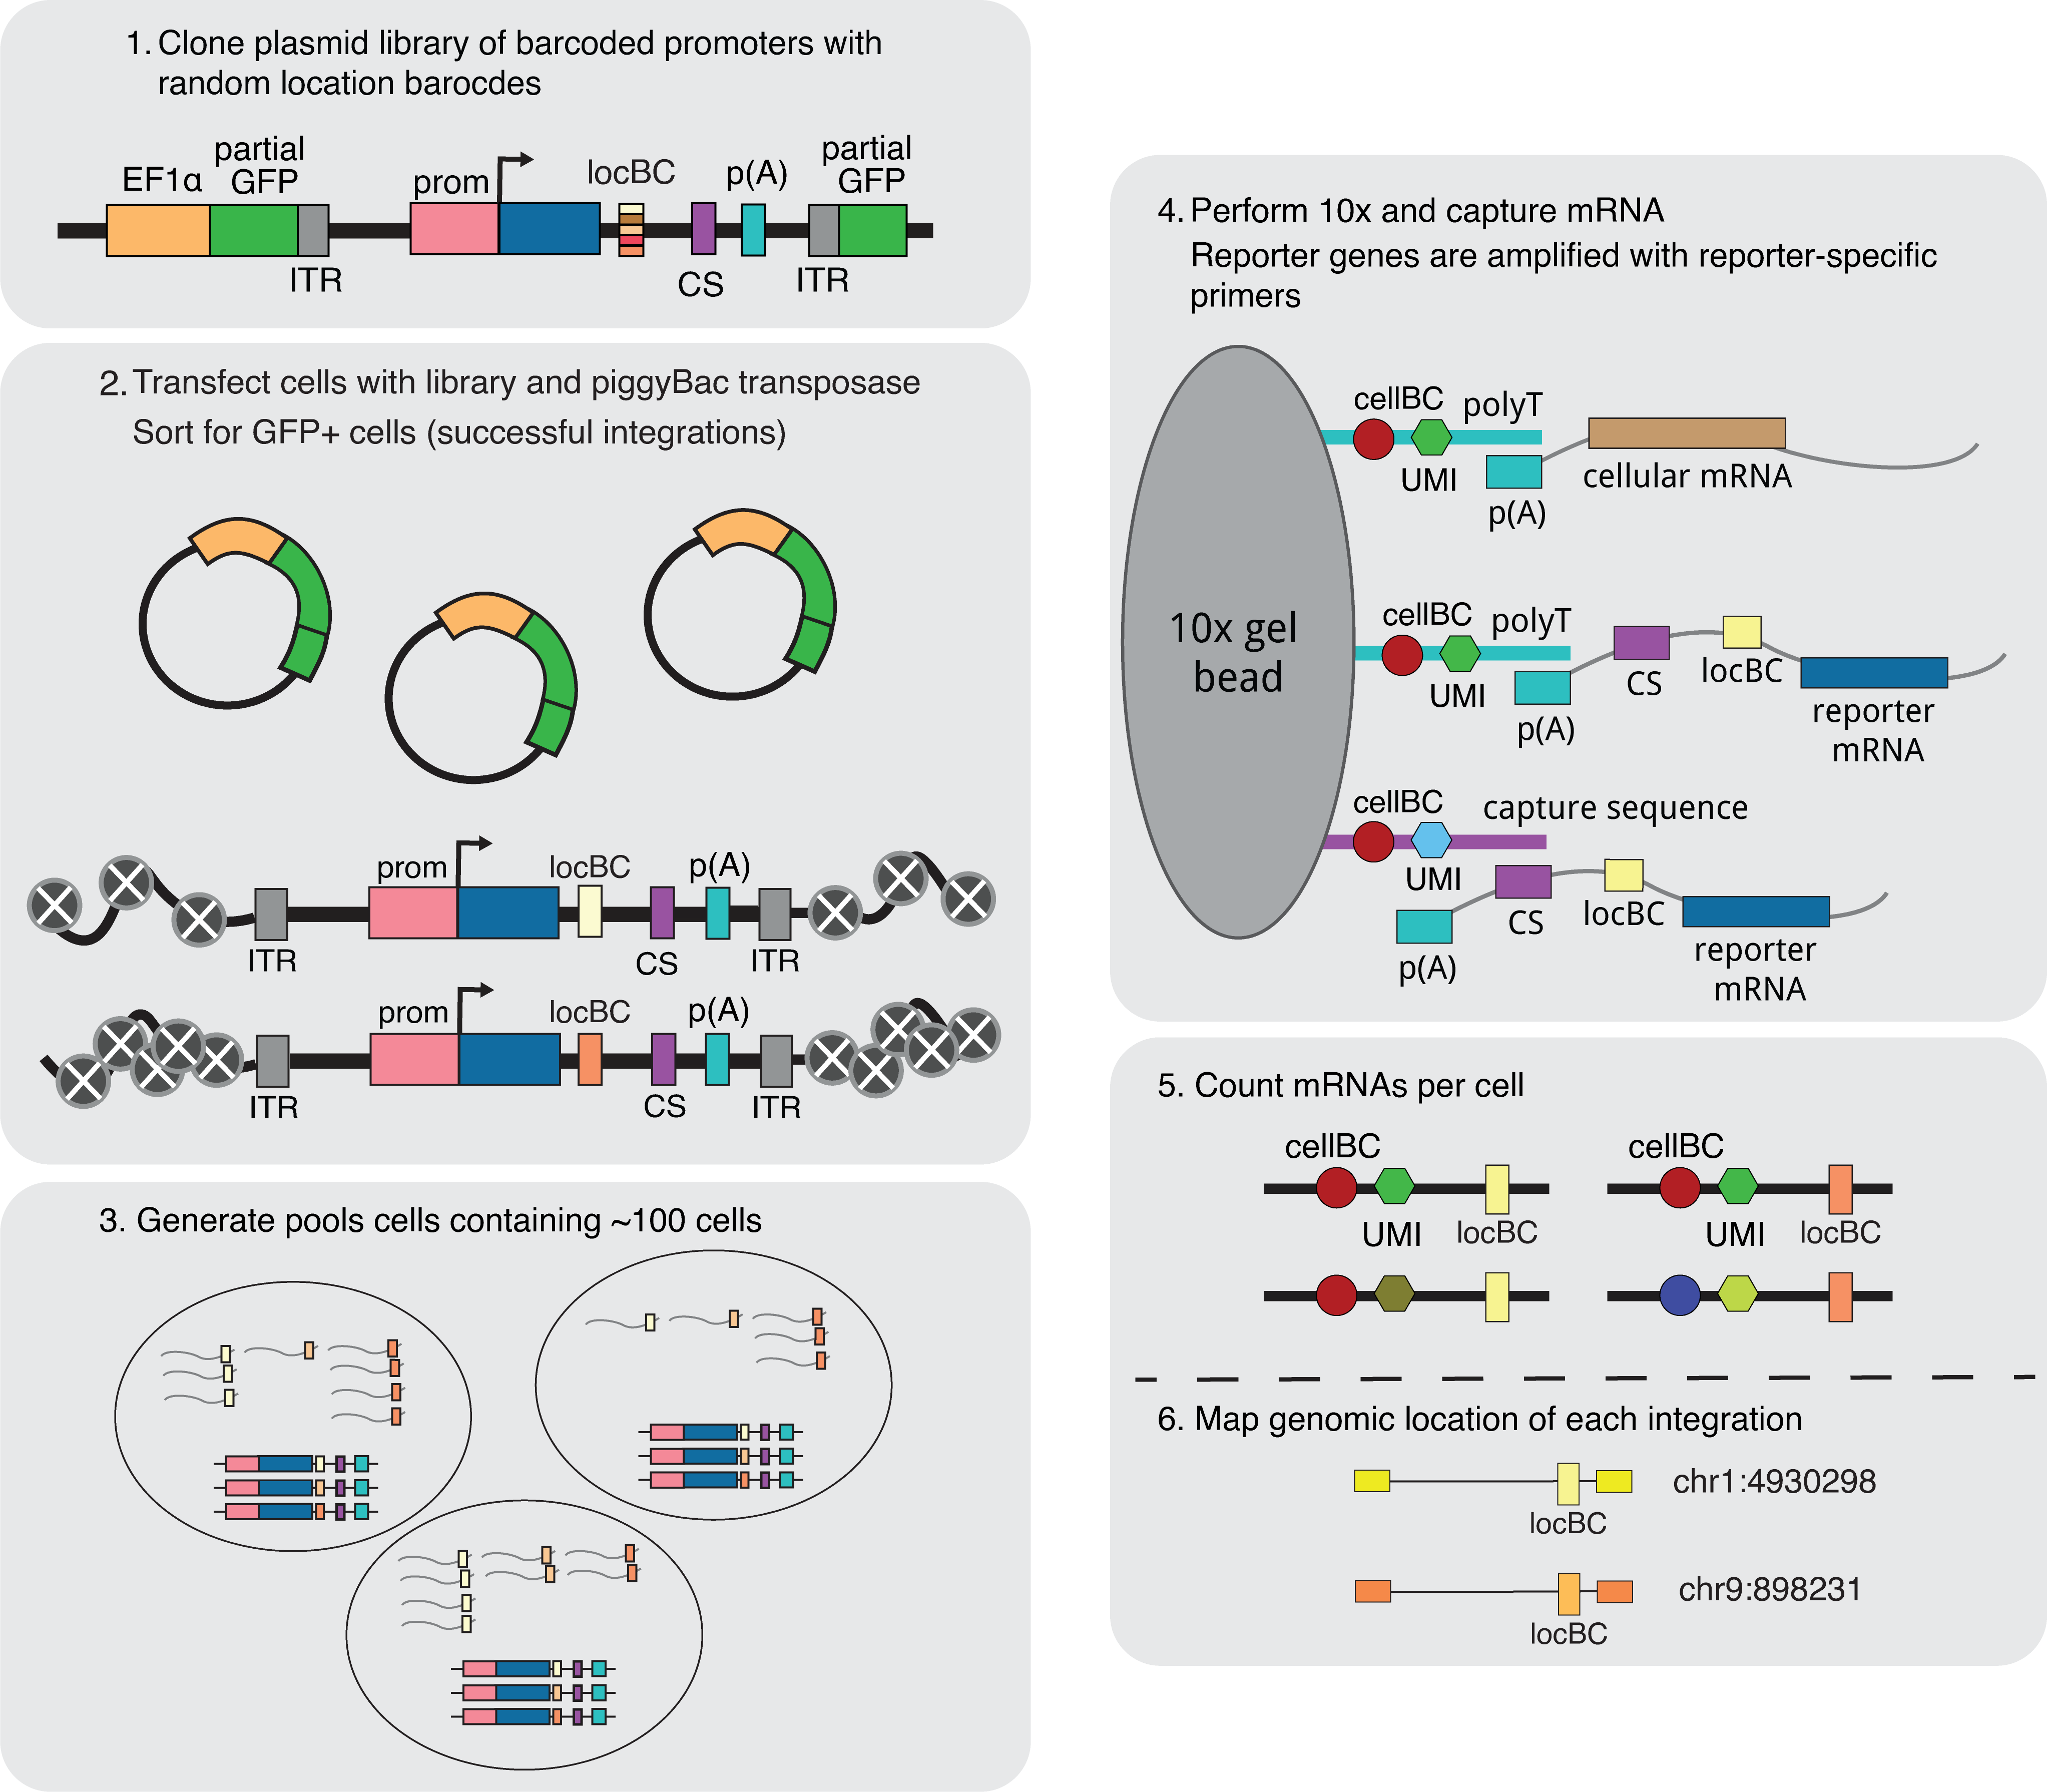
\includegraphics[width=\linewidth]{figures/cas_figure1.png}
    \caption[Overview of the SARGENT workflow.]{%
        \textbf{Overview of the SARGENT workflow.}
         In step 1, a reporter gene driven by the CMV promoter is randomly barcoded with a diverse library of location barcodes (locBC) upstream of the 10x capture sequence (CS). The reporter genes are randomly integrated into K562 cells and sorted for cells with successful integrations (step 2), then sorted again after a week into pools to ensure that each barcode is only represented once per pool (step 3). We then performed scRNA-seq to capture the transcriptome and amplify the expressed barcodes from integrated reporter genes (step 4). The number of expressed barcodes per cell were then tabulated (step 5). To identify the genomic locations of the integrations we also mapped the location of each locBC in bulk (step 5). (ITR = Inverted terminal repeat; prom = promoter)
    }
    \label{fig:cas_figure1}
\end{figure}

To generate chromosomal integrations across the genome we cloned the reporter gene library onto a piggyBac transposon vector. The library was transfected into cells along with piggyBac transposase to allow random integrations of the reporter into the genome. After selecting for integrations in K562 cells, we mapped the locations of each integrated reporter (IR) and assigned each locBC to a specific genomic location. We then captured the reporter gene transcripts from single cells and amplified the barcodes (10x cell barcode, UMI, and locBC) using primers specific to our reporter gene (\hyperref[section:cas_methods]{Methods}). After sequencing and tabulating the mRNA counts for each IR we computed the expression level of the reporter gene at each genomic location in each single cell. For a subset of cells we also sequenced the mRNA profiles to simultaneously reveal the cell state of each individual cell.

\subsection{SARGENT measurements are accurate and reproducible}

We performed SARGENT in K562 cells because of the abundance of public epigenetic data available for this cell line. We first assessed the reproducibility of the SARGENT method. Because replicate infections result in pools of cells with insertions at different genomic locations, we could not assess the reproducibility of independently transfected pools of cells. Instead, we assessed the reproducibility of SARGENT by growing the same pool of insertions twice and performing the SARGENT workflow independently on each sample. We detected 589 identical IR locations in both replicates, which represented 96\% of the total IRs observed in both replicates. After quality control, we obtained data from 7680 single cells across replicates, and a total of 2,940,912 unique molecular identifiers (UMIs) representing expressed barcodes from the IRs in these cells. The replicates were well correlated for measurements of both mean and noise measured at each IR location (\fref{fig:cas_figure2a}-\subcaptionref{fig:cas_figure2b}, mean Pearson’s \textit{r} = 0.76, noise Pearson’s \textit{r} = 0.72) indicating that measurements obtained by SARGENT are reproducible.

%figure2
\begin{figure}[tb]  
    \centering
    \phantomlabel{fig:cas_figure2a}
    \phantomlabel{fig:cas_figure2b}
    \phantomlabel{fig:cas_figure2c}
    \phantomlabel{fig:cas_figure2d}
    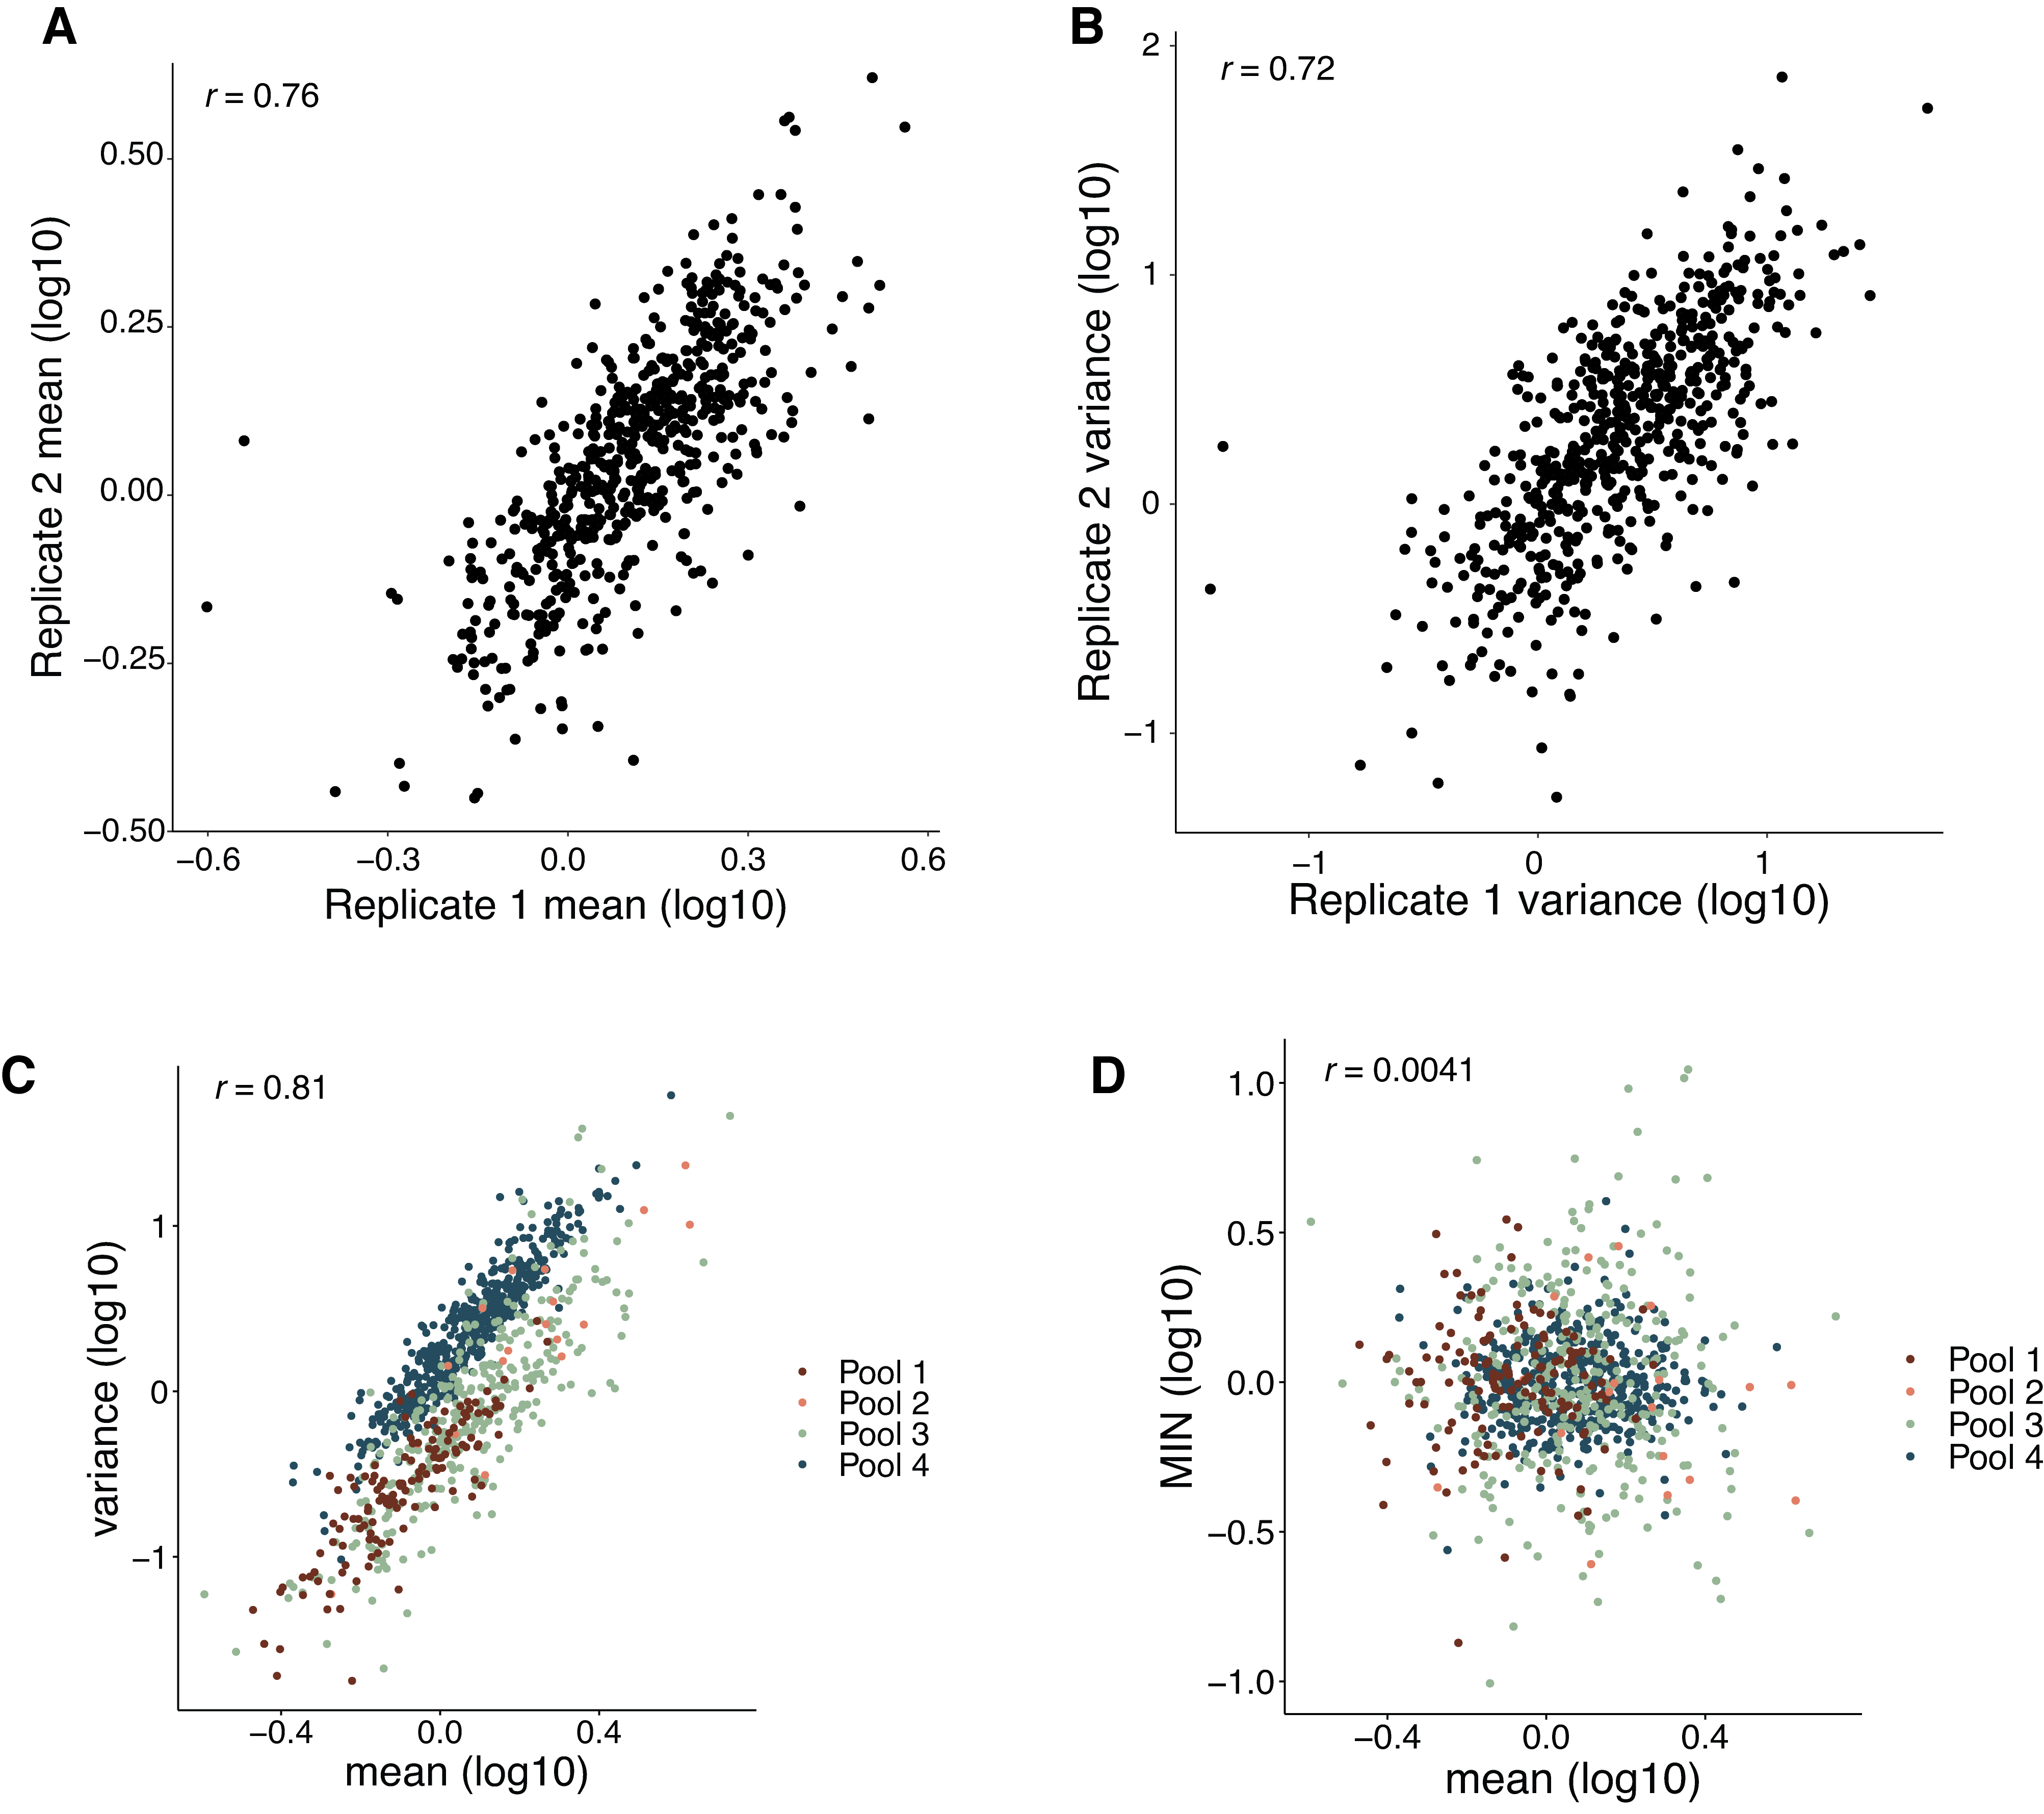
\includegraphics[width=\linewidth]{figures/cas_figure2.ai}
    \caption[SARGENT measurements are accurate and reproducible.]{%
        \textbf{SARGENT measurements are accurate and reproducible.}
        \subref{fig:cas_figure2a}
        Correlation of mean levels between technical replicates.
        \subref{fig:cas_figure2b}
        Correlation of variance measurements between replicates.
        \subref{fig:cas_figure2c}
        Mean and variance are correlated within each experiment.
        \subref{fig:cas_figure2d}
        Mean-independent noise corrects for mean effects on variance. Correlations shown are Pearson’s correlation coefficients (Pearson’s \textit{r}). 
    }
    \label{fig:cas_figure2}
\end{figure}

To validate the single-cell measurements made by SARGENT, we also performed single-molecule Fluorescence In Situ Hybridization (smFISH) on two known locations. The measurements of mean and noise made by smFISH agree with the SARGENT measurements for those locations (\fref{fig:cas_figureS1}) demonstrating that our method is accurate and reproducible for measuring the mean and noise of expression. 

\subsection{Measurements of mean-independent noise across different chromosomal environments}

In total, we performed four experiments and generated mean and noise measurements for 939 integrations. The integrations were spread across the genome and found in regions with different chromHMM annotations \cite{ernstj_kellism:DiscoveryCharacterization2010} (\fref{fig:cas_figureS2a}-\subcaptionref{fig:cas_figureS2b}), allowing us to study the effects of diverse chromosomal environments on expression noise.

The mean and noise of expression are often highly correlated \cite{vallaniaflm_mitrard:OriginConsequences2014,bar-evena_barkain:NoiseProtein2006}. Similarly, we found a strong correlation between the mean and noise in SARGENT data, indicating that a large proportion of an IR’s noise is explained by its mean level of expression (\fref{fig:cas_figure2c}). To identify chromosomal features that control expression noise independent of mean levels we regressed out the effect of mean levels on noise, leaving us with a metric we refer to as mean-independent noise (MIN) \cite{vallaniaflm_mitrard:OriginConsequences2014}. By design, MIN levels of IRs are uncorrelated with their mean expression levels (\fref{fig:cas_figure2d}) whereas other measures of noise, such as the coefficient of variance or the Fano factor, retain residual correlation with mean levels in our data (\fref{fig:cas_figureS2c}-\subcaptionref{fig:cas_figureS2d}). Thus, we used MIN as a measure of expression noise for all following analyses.

\subsection{Expression mean and noise are associated with different chromosomal features}

We sought to identify chromatin features that would explain differences in MIN levels between genomic locations. Studies of genome-wide chromatin features in many cell lines and tissues have shown that the mean expression of a gene is correlated with its surrounding chromatin marks \cite{dunham2012n, akhtarw_vansteenselb:ChromatinPosition2013}. Thus, we asked whether chromatin features might also explain patterns of MIN across the genome. We split the IRs into bins of high or low mean levels, or high or low MIN levels, and identified chromatin features that were enriched in specific bins. As expected, IRs with high mean expression had higher levels of active chromatin marks such as H3K27ac, H3K4 methylation, H3K79me2 and H3K9ac (\fref{fig:cas_figure3a}). Conversely, IRs with high MIN did not exhibit significant differences between H3K27ac or H3K4me1 levels, and low MIN locations showed slightly elevated levels of H3K4me2/3, H3K79me2 and H3K9ac (\fref{fig:cas_figure3b}). These results suggest that different chromatin modifications influence the mean and noisiness of expression, and that more active genomic locations might also reduce MIN. This observation is consistent with previous studies showing that repressed chromatin is associated with high MIN \cite{faureaj_lehnerb:SystematicAnalysis2017,deyss_arkinap:OrthogonalControl2015}. 

%figure3
\begin{figure}[tbp]  
    \centering
    \phantomlabel{fig:cas_figure3a}
    \phantomlabel{fig:cas_figure3b}
    \phantomlabel{fig:cas_figure3c}
    \phantomlabel{fig:cas_figure3d}
    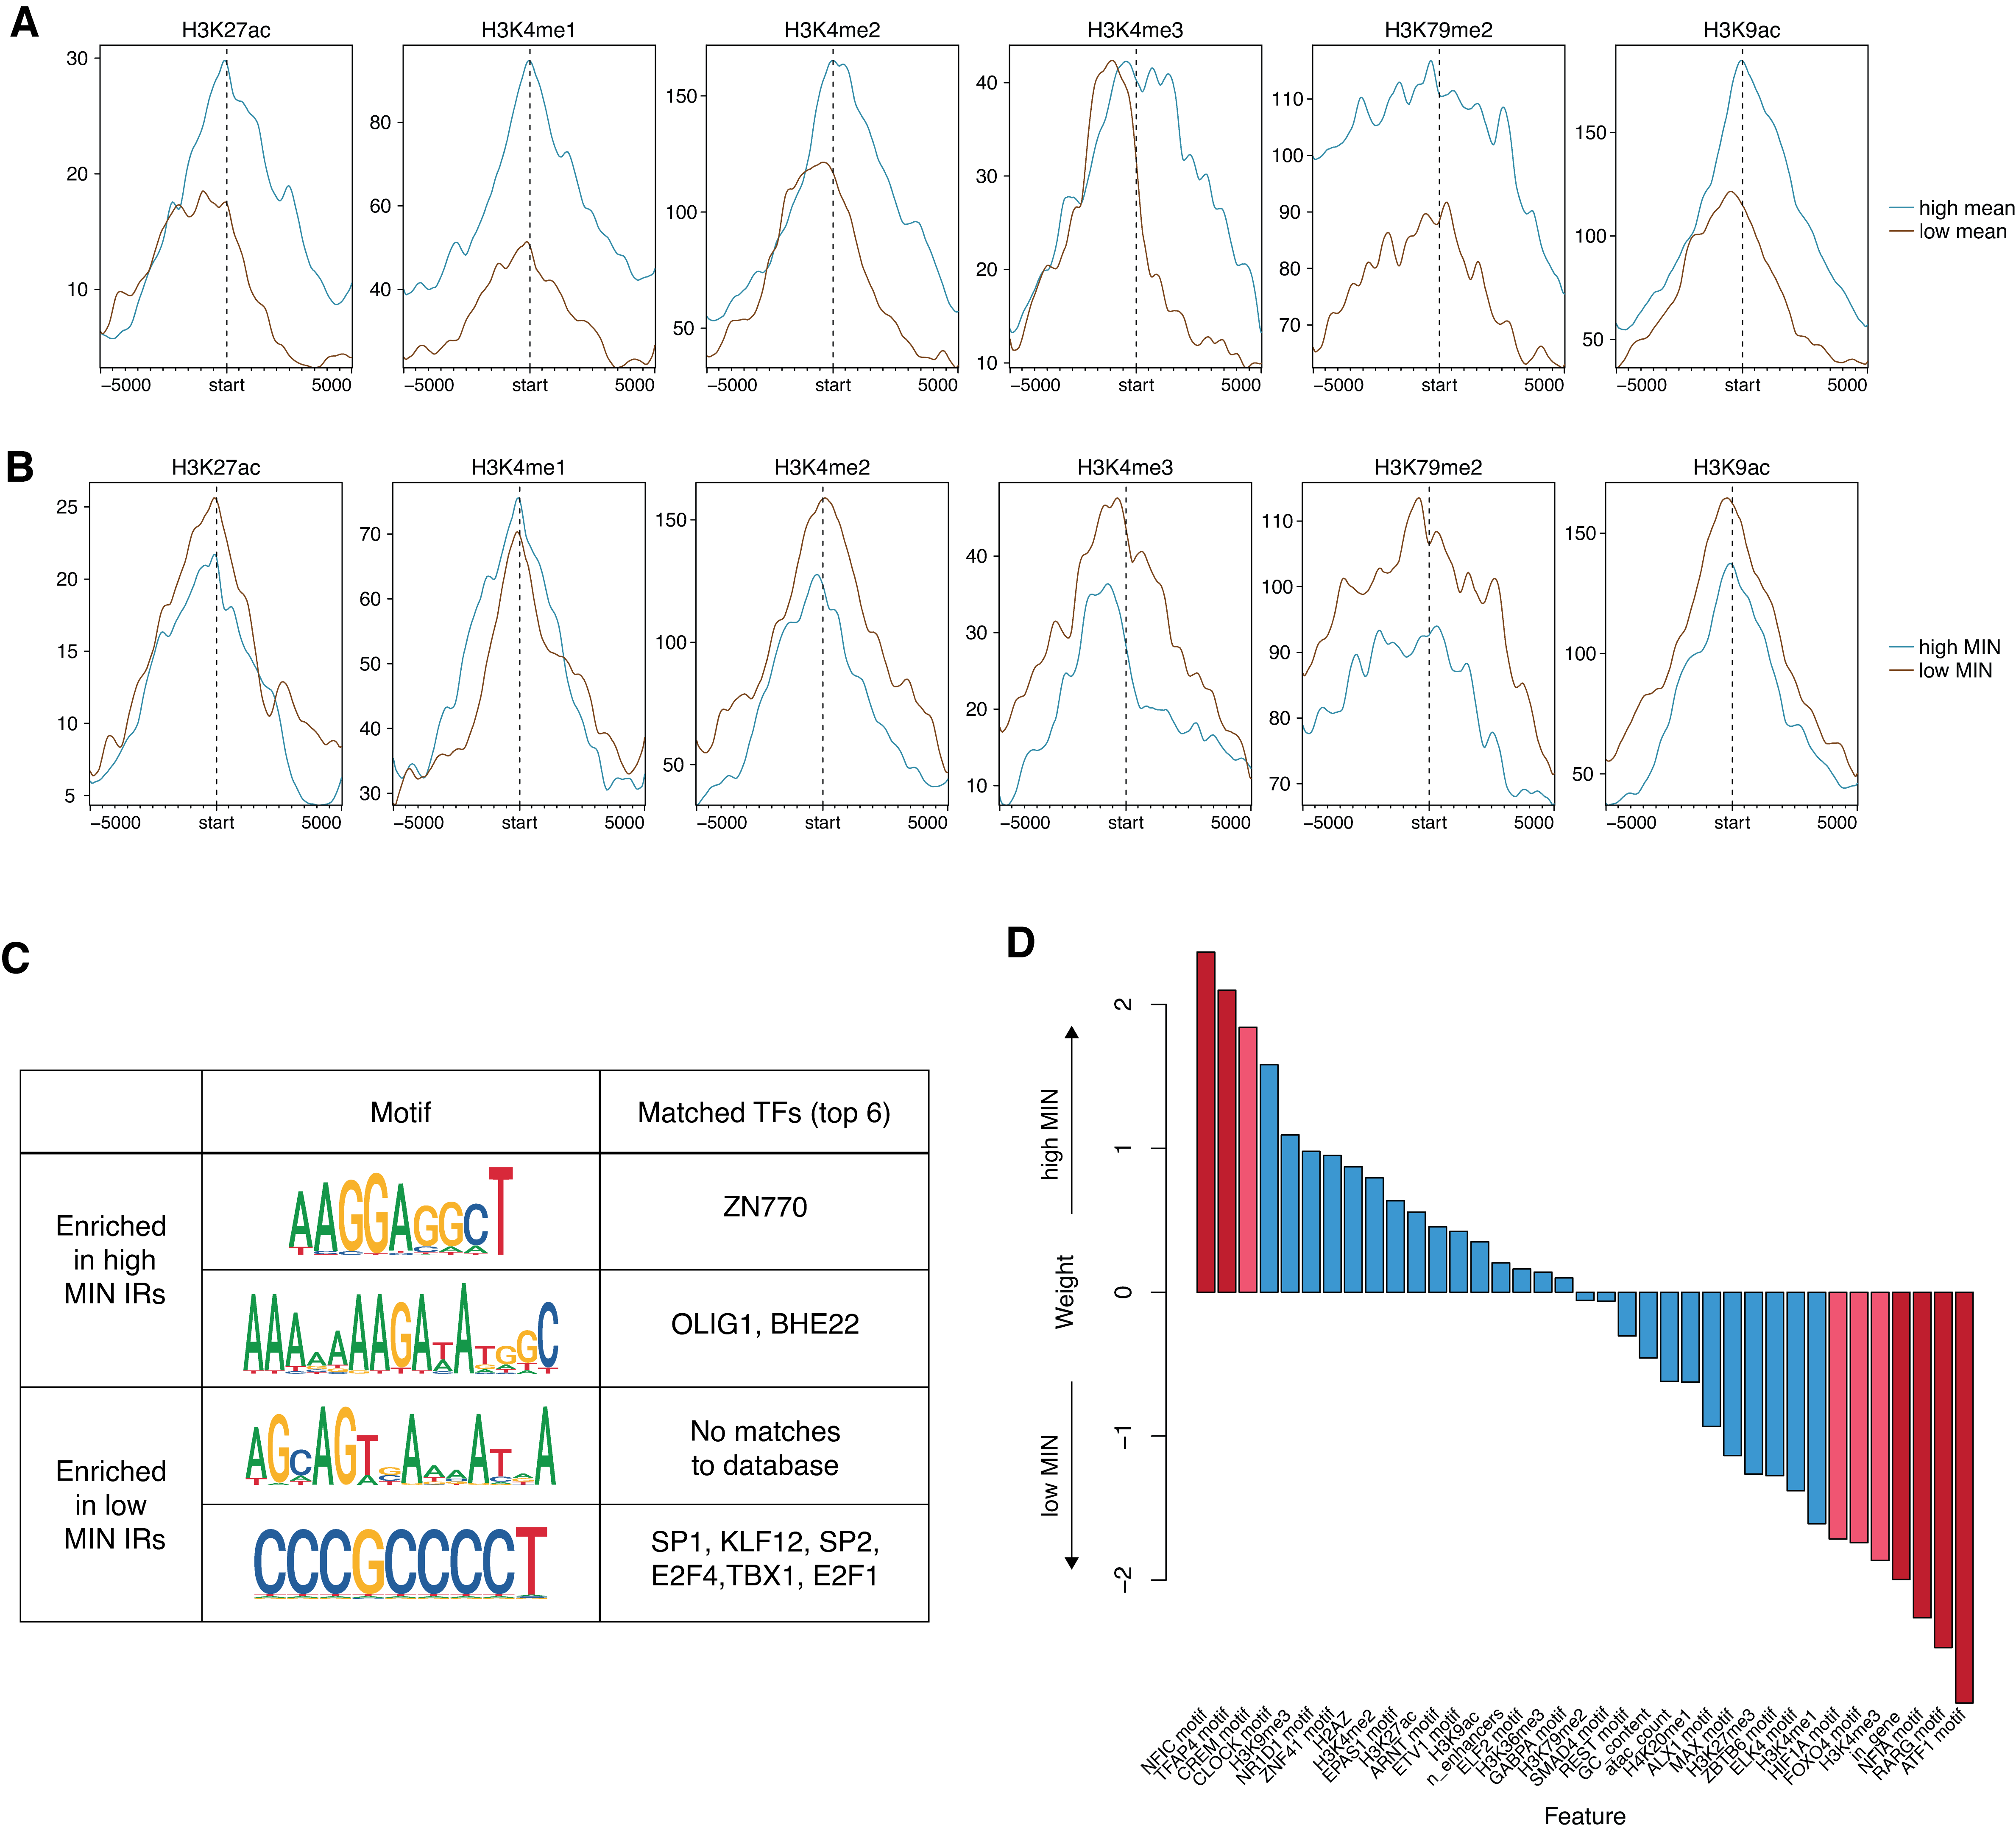
\includegraphics[width=\linewidth]{figures/cas_figure3.ai}
    \caption[Chromosomal features associated with expression mean and noise.]{%
        \textbf{Expression mean and noise are associated with different chromosomal features.}
        \subref{fig:cas_figure3a}
        Active histone modifications associated with high or low mean IRs. Start indicates the location of the IR, and each location was extended 5kb on either side.
        \subref{fig:cas_figure3b}
        Active histone modifications associated with high or low MIN IRs are different from those associated with mean.
        \subref{fig:cas_figure3c}
        Motifs enriched in high or low MIN IRs respectively, and potential TFs that match these discovered motifs.
        \subref{fig:cas_figure3d}
        Logistic regression weights of various intrinsic features associated with high or low MIN IRs. Red bars: \textit{p}-value $<$ 0.05; Pink bars: 0.05 $<$ \textit{p}-value $<$ 0.1 from the logistic regression model.  
    }
    \label{fig:cas_figure3}
\end{figure}

The binding of TFs also impacts noise in gene expression. To identify TFs that might affect noise, we identified TFs whose occupancy is enriched near either high or low MIN IRs. Sequences at low MIN IRs are enriched for transcriptional activators such as SP1 and E2F4, while sequences at high MIN IRs are enriched for other TFs including TFs containing basic helix-loop-helix (bHLH) domains (\fref{fig:cas_figure3c}), suggesting that the cofactors recruited by different TFs have separable effects on expression mean and noise. 

To assess the power of genomic features to predict the MIN of IR locations we trained a logistic regression model using chromatin modifications and DNA sequence features to classify high and low MIN locations and achieved an accuracy of 76\%. When applied to data from a different pool, the trained model achieved 67\% accuracy. The features with significant weights are the H3K4me3 mark, TF motifs (RARG, FOXO4, HIF1A, TFAP4, CREM, ATF1, NFIC, and NFIA) and whether the IR location was inside a gene (\fref{fig:cas_figure3d}). Being inside a gene reduced the probability of being a high noise lR location, which could be due to local regulatory elements that dampen the noisiness of a gene’s expression. Similar to our results above, lower H3K4me3 increased the probability of being a high noise IR location. H3K4me3 is associated with active chromatin and supports the hypothesis that higher activity reduces IR MIN. Our observation is consistent with a previous study showing that H3K4me3 correlates with reduced noise at endogenous genes \cite{faureaj_lehnerb:SystematicAnalysis2017}. With respect to the effects of TFs on noise, the presence of some TF motifs increase the probability of being a high noise IR location (NFIC, CREM, TFAP4, CLOCK), whereas other TFs reduce the probability of being a high noise location (RARG, NFIA, ATF1, FOXO4, HIF1A). 

We used a similar logistic regression framework to identify features that separate IR locations with high or low mean levels of expression and achieved an accuracy of 82\%. When applied to holdout data, the trained model achieved 62\% accuracy. The chromatin features that increase the probability of being a high mean IR location are lower levels of H3K27me3, lower levels of H3K4me2 and a higher number of ATAC-seq peaks, which agrees with the known effects of these features in bulk mean expression. The motifs that increased the probability of being a high mean IR location are higher numbers of motifs of the ZNF76, BACH1 and E2F3 TFs and fewer instances of the E2F7, SMAD3 and SOX5 motifs (\fref{fig:cas_figureS3}). Comparisons of the models explaining either mean or noise again show that different genomic features are correlated with gene expression mean and noise.

\subsection{Intrinsic and extrinsic factors have similar effects on gene expression noise}

Expression noise caused by fluctuations in global factors affects all genes and is referred to as extrinsic noise, whereas intrinsic sources of noise are specific to individual genes \cite{deyss_arkinap:OrthogonalControl2015, stewart-ornsteinj_el-samadh:CellularNoise2012, sancheza_goldingi:GeneticDeterminants2013, raserjm_osheaek:ControlStochasticity2004, zopfcj_maheshrin:CellCycleDependence2013, vallaniaflm_mitrard:OriginConsequences2014}. The correlation between identical reporter genes in the same cell measures the balance between extrinsic and intrinsic noise, with extrinsic factors increasing the correlation \cite{elowitzmb_swainps:StochasticGene2002}. In SARGENT, the correlation between IRs in the same cells is a measure of extrinsic factors that affect noise across IR locations. 

For our analysis of extrinsic noise we first identified IRs in the same clonal cells using the co-occurrence of locBCs between single cells (\fref{fig:cas_figure4a}). We identified 192 clones, with a mean of three integrations per clone (\fref{fig:cas_figureS4a}). Of these 192 clones, 45 contain more than one integration (\fref{fig:cas_figure4b}), making them suitable for an analysis of extrinsic noise. To validate the identified clones, we individually mapped IR barcodes in sixteen clones and found that 94\% of the individually mapped IR locations could be uniquely assigned to an identified clone (\fref{fig:cas_figure4b}). 

%figure4
\begin{figure}[tbp]  
    \centering
    \phantomlabel{fig:cas_figure4a}
    \phantomlabel{fig:cas_figure4b}
    \phantomlabel{fig:cas_figure4c}
    \phantomlabel{fig:cas_figure4d}
    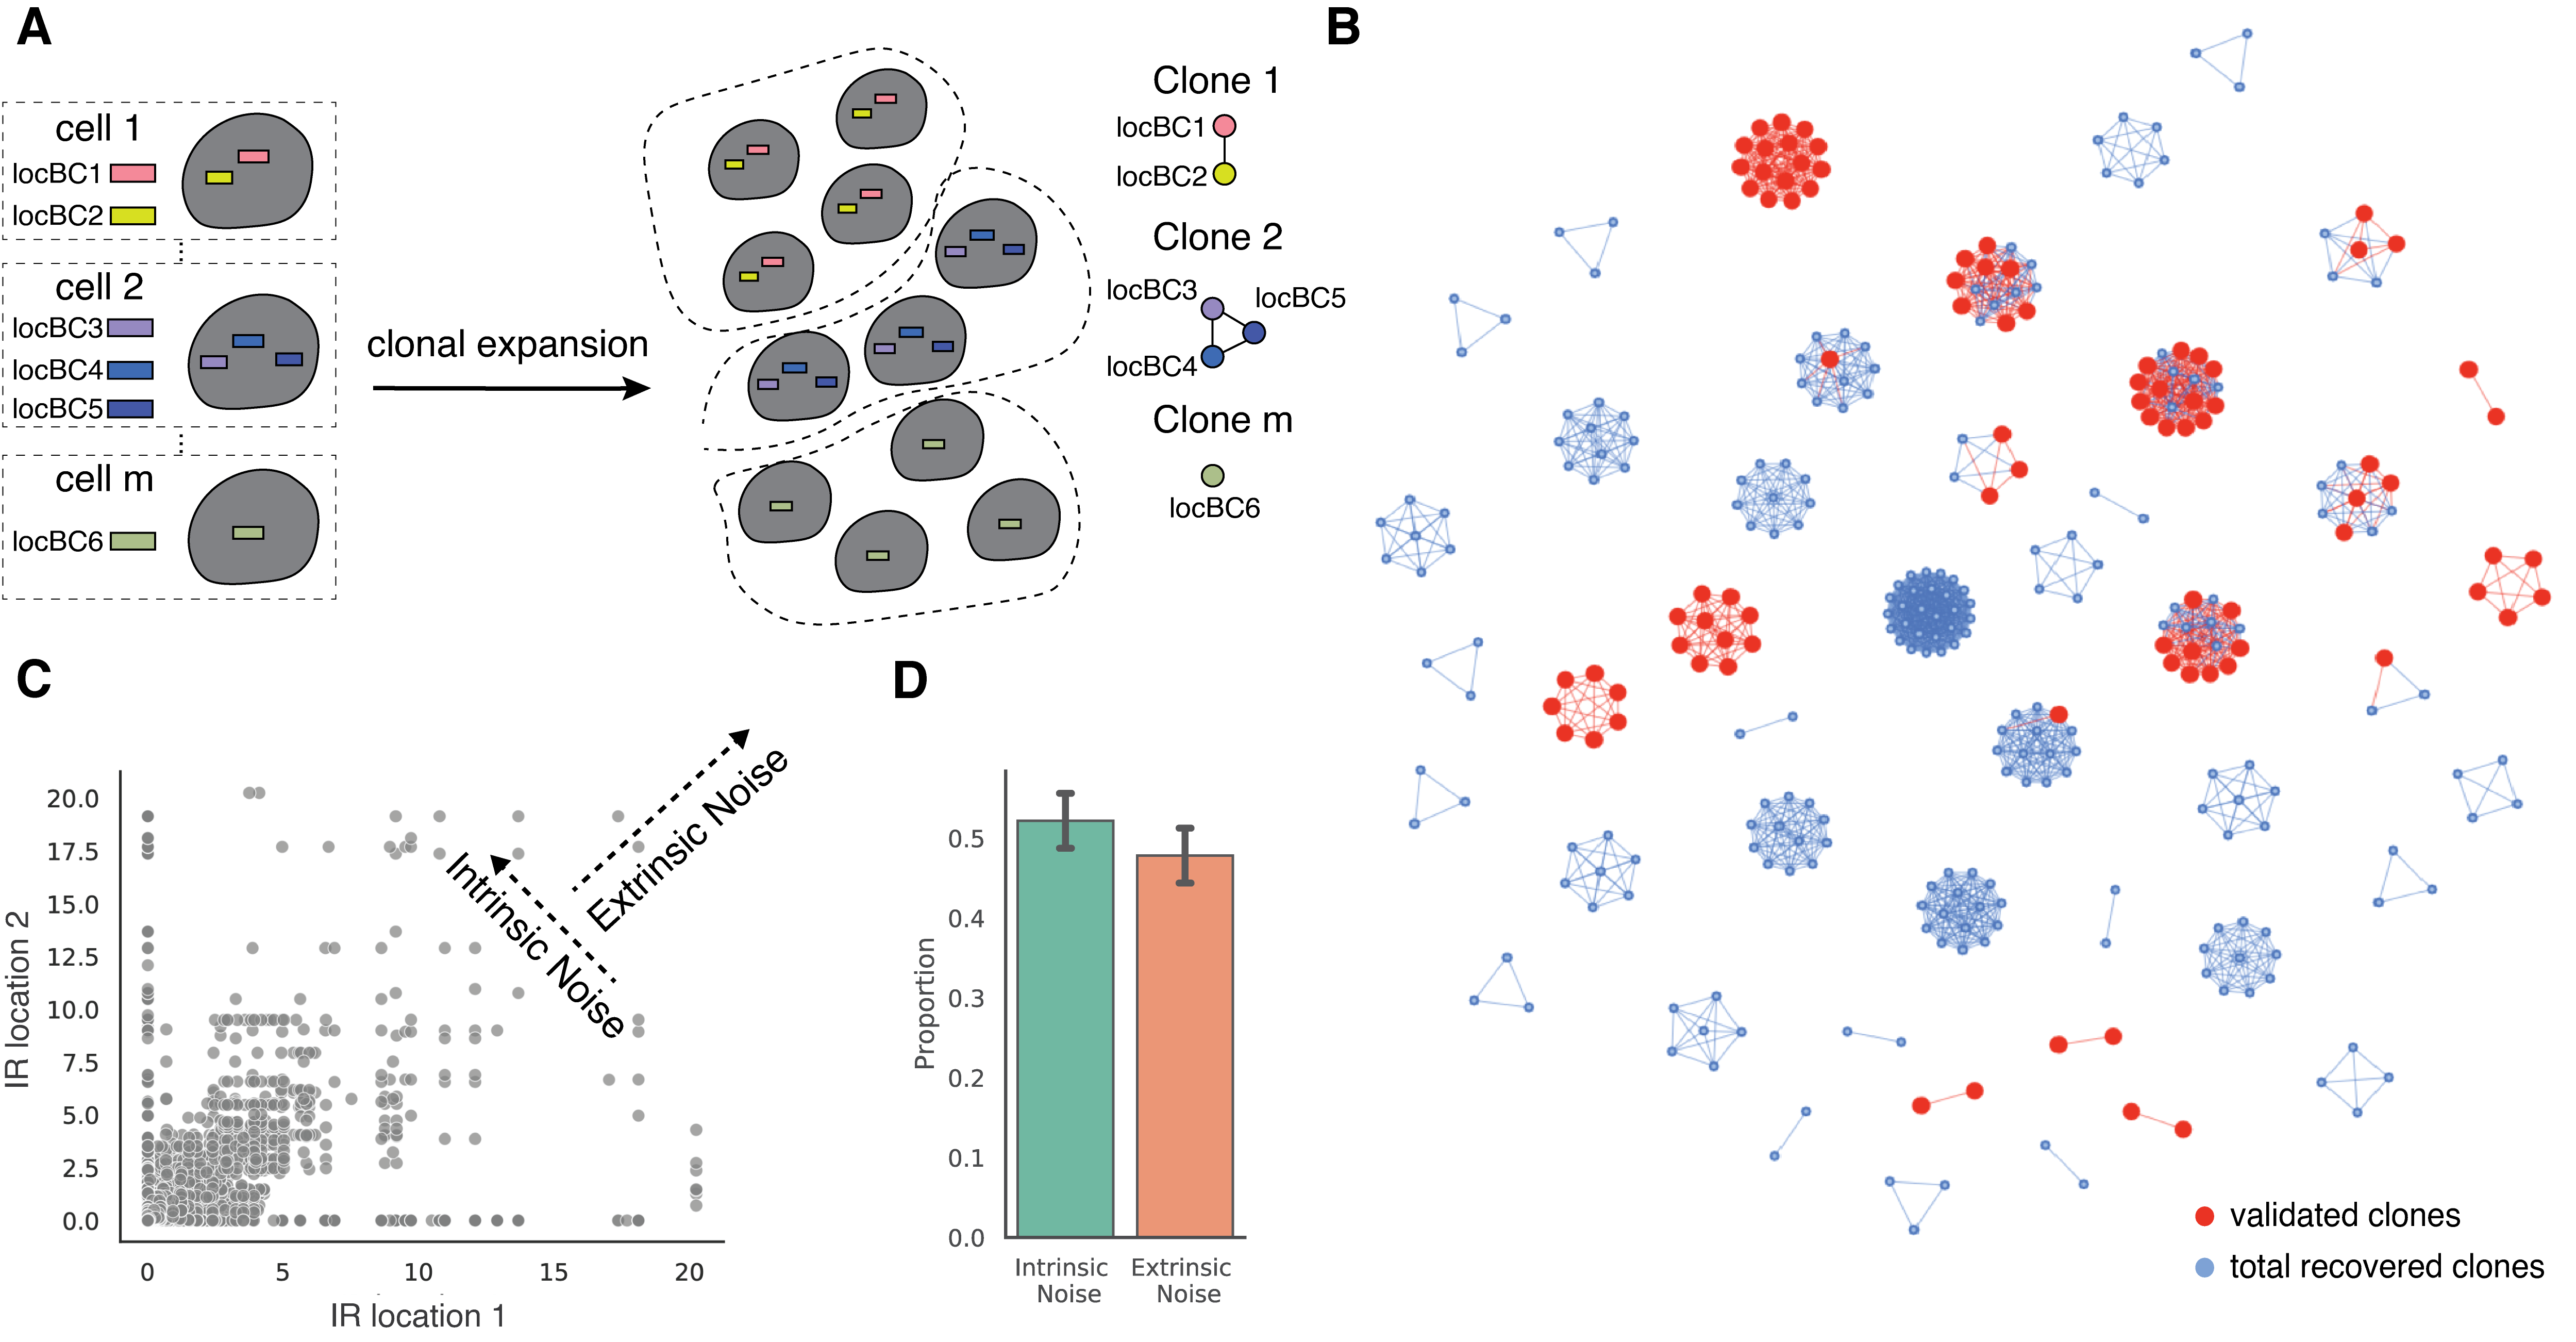
\includegraphics[width=\linewidth]{figures/cas_figure4.ai}
    \caption[SARGENT quantifies the extrinsic portion of expression noise.]{%
        \textbf{SARGENT quantifies the extrinsic portion of expression noise.}
        \subref{fig:cas_figure4a}
        Schematic for identifying different initial TRIP clones.
        \subref{fig:cas_figure4b}
        A network representation of the different clones identified, red nodes indicate IR locations that were independently validated by sequencing individual clones.
        \subref{fig:cas_figure4c}
        Pairwise expression for any two IR locations observed in the same cell. The trend along the diagonal suggests the existence of extrinsic noise, and the anti-correlation indicates the amount of intrinsic noise.
        \subref{fig:cas_figure4d}
        Quantification of intrinsic and extrinsic proportion of noise. Error bars from two technical replicates. 
    }
    \label{fig:cas_figure4}
\end{figure}

We next asked if extrinsic factors also contribute to the observed gene expression noise. For each cell in a clone, we calculated the standard deviation relative to the mean of all IRs in that cell, which we define as the fluctuation index. Lower fluctuation indices indicate that the IRs in a clone fluctuate in sync (high extrinsic noise), while higher fluctuation indexes indicate that each IR varies independently (high intrinsic noise). To simulate intrinsic noise, we first shuffled the cell labels of all the IRs within a clone and computed a distribution of fluctuation indexes for the shuffled population. If all the measured noise was intrinsic, then the measured distribution would perfectly overlap the shuffled distribution. If all the measured noise was extrinsic, then all the cells would have fluctuation indexes of 0 (\fref{fig:cas_figureS4b}). We found that all clones show a distribution of fluctuation indexes that is lower than that of the shuffled distribution and above zero (\fref{fig:cas_figureS4c}). This suggests that some portion of the expression noise can be explained by extrinsic factors that impact all IRs within a cell in different genomic environments.

To quantify the contribution of intrinsic and extrinsic noise in each clone we employed an established statistical framework \cite{fuaq_pachterl:EstimatingIntrinsic2016}. Using the pairwise IR single cell expressions for all clones that contain more than one IR as input, we found that intrinsic noise comprises approximately 54\% of the total noise (\fref{fig:cas_figure4c}-\subcaptionref{fig:cas_figure4d}). This analysis suggests that both the intrinsic chromatin and extrinsic cellular context explains about half of the total noise in each clone. These results show that SARGENT can quantify both intrinsic and extrinsic contributions to expression noise.

\subsection{Cell substates are a source of expression noise}

What cellular mechanisms control expression noise? We hypothesized that differences between cellular substates within isogenic populations are an important source of noise. Isogenic K562 cells transition between \enquote{stem-like} and \enquote{more differentiated} substates \cite{litzenburgerum_changhy:SinglecellEpigenomic2017, moudgila_mitrard:SelfReportingTransposons2020}. The stem-like substate is marked by high CD24 expression and proliferates at a higher rate, which we hypothesized would contribute to extrinsic noise. This hypothesis predicts that the same IRs will have higher MIN in stem-like cells compared to more differentiated cells. To test this prediction we sequenced the single-cell transcriptomes associated with 356 of the 939 genomic locations in parallel with the IRs. Using the transcriptomes we identified clusters of cells with high CD24 expression and confirmed that these clusters had the signatures of high-proliferating cells (\fref{fig:cas_figureS5a}-\subcaptionref{fig:cas_figureS5b}). We then calculated the expression mean and MIN for each IR location separately in the two substates. IR locations in the stem-like substate have higher mean and lower MIN (\fref{fig:cas_figure5a}-\subcaptionref{fig:cas_figure5b}) suggesting that the global differences between the two substates are a source of MIN. 

%figure5
\begin{figure}[tbp]  
    \centering
    \phantomlabel{fig:cas_figure5a}
    \phantomlabel{fig:cas_figure5b}
    \phantomlabel{fig:cas_figure5c}
    \phantomlabel{fig:cas_figure5d}
    \phantomlabel{fig:cas_figure5e}
    \phantomlabel{fig:cas_figure5f}
    \phantomlabel{fig:cas_figure5g}
    \phantomlabel{fig:cas_figure5h}
    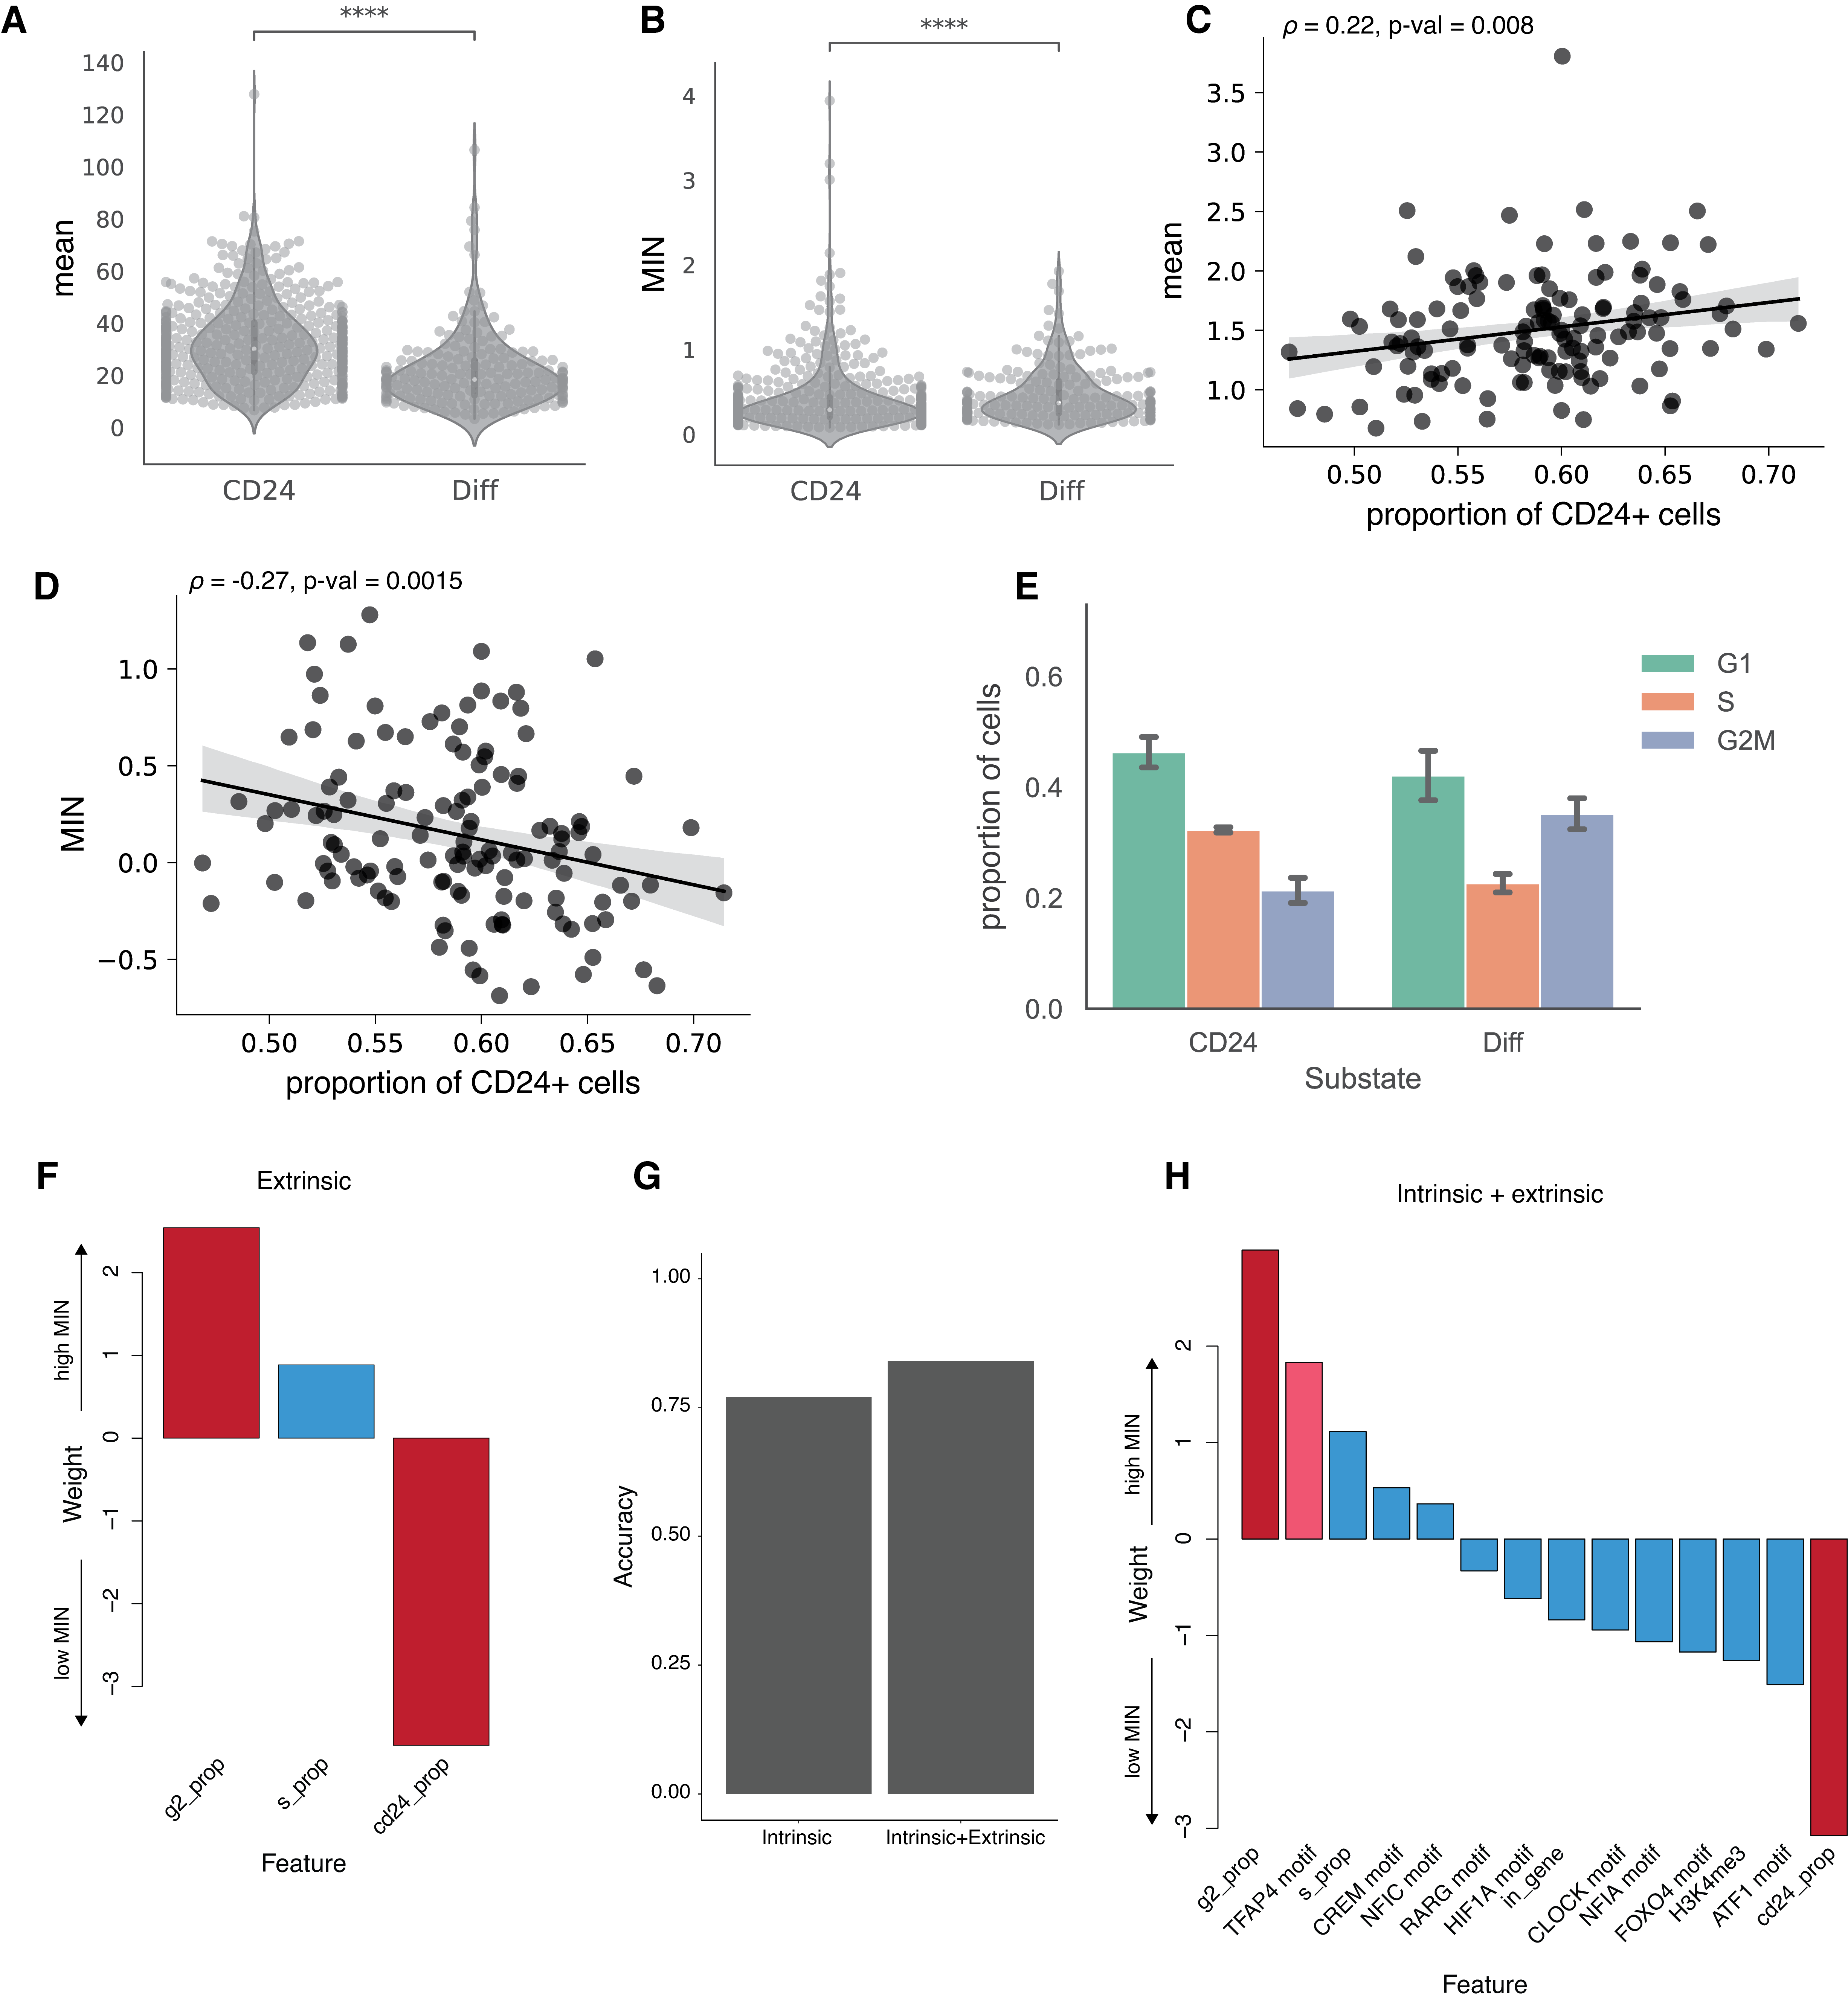
\includegraphics[width=\linewidth]{figures/cas_figure5.ai}
    \caption[Cellular information improves classification of MIN IR locations.]{%
        \textbf{Cellular information improves classification of low vs high MIN IR locations. (A,B)}
        Violin plots of expression mean \subref{fig:cas_figure5a} and MIN \subref{fig:cas_figure5b} at two substates (student t-test, $\ast\ast\ast\ast$: \textit{p} <  0.0001), each dot is an IR location.
        \textbf{(C,D)}
        Scatterplots of proportion of cells in the \enquote{stem-like} substate against mean \subref{fig:cas_figure5c} and MIN \subref{fig:cas_figure5d}. Each dot is the average mean expression or MIN from a clone. Line: linear fit with 95\% confidence interval. 
        \legendcontdnote
    }
    \label{fig:cas_figure5}
\end{figure}

\begin{figure}[t]
    \centering
    \legend{%
        \legendcontdref{fig:cas_figure5}
        \subref{fig:cas_figure5e}
        Barplot of the fraction of cells in different cell cycle phases for cells in the \enquote{stem-like} substate and the \enquote{differentiated} substate (Binomial test: S phase \textit{p} $<$ 2.2e-16, G1 phase \textit{p} $<$ 5.9e-5, G2M phase \textit{p} $<$ 2.2e-16). The error bars are derived from the two replicates.
        \subref{fig:cas_figure5f}
        Weights of logistic regression model using extrinsic (cellular) features alone.
        \subref{fig:cas_figure5g}
        Addition of extrinsic features helps to improve the accuracy of the model.
        \subref{fig:cas_figure5h}
        Weights of logistic regression model using both intrinsic and extrinsic features. The most significant features are still the proportion of cells in the G2 phase and CD24+ phase. Red bars: \textit{p}-value $<$ 0.05; Pink bars: 0.05 $<$ \textit{p}-value $<$ 0.1 from the logistic regression model. 
    }
\end{figure}

Given the differences in mean and MIN between the substates, the MIN of the IR locations in a given clone should be partly explained by the proportion of its cells in each substate. Consistent with this prediction, we found that clones with a higher proportion of cells in the stem-like substate have slightly higher average mean expression (Spearman’s \textit{ρ} = 0.22, \textit{p}-value = 0.008), and lower average MIN (Spearman’s \textit{ρ} = -0.27, \textit{p}-value = 0.0015) across all IRs in the clone (\fref{fig:cas_figure5c}-\subcaptionref{fig:cas_figure5d}). We hypothesized that this was due to the slightly higher proliferation rates of cells in the stem-like phase. As expected, there are more cells in the S phase in the stem-like substate compared to the more differentiated state (\fref{fig:cas_figure5e}). We then examined the differences of mean and MIN in different cell cycle phases and found that expression mean is higher and MIN is lower in the S phase compared to other phases (\fref{fig:cas_figureS5c}-\subcaptionref{fig:cas_figureS5d}). These results suggest that differences in proliferation rates is an important source of extrinsic noise, and that SARGENT is a powerful tool to dissect the extrinsic sources of expression noise. 

\subsection{Cellular information improves classification of low vs high MIN IR locations}

Since extrinsic factors play an important role in determining expression noise, we trained a logistic regression model to predict MIN using three extrinsic features (proportion of cells in S, proportion of cells in G2, and proportion of CD24+ cells). Using only the global features, the model achieved 75\% accuracy (albeit without a holdout set to test on due to the small numbers of locations with associated extrinsic features). This result implies that these cellular features explain a significant portion of the variance in MIN between high and low IR locations. The proportion of cells in G2 and the proportion of cells in the CD24+ state were significant predictors in this model. Being in G2 increases the probability of a high MIN IR location whereas having a higher proportion of CD24 cells reduced the probability of being a high MIN IR location (\fref{fig:cas_figure5f}). When we combined the significant intrinsic features from the previous model with these extrinsic features, the model accuracy increased to 84\% (\fref{fig:cas_figure5g}). In the combined model, the extrinsic features have higher weights than the intrinsic genomic environment features (\fref{fig:cas_figure5h}), suggesting that the cell-state information may play a larger role in regulating MIN compared to genomic environments. 

We observed a similar role for extrinsic features in classifying IR locations with high mean levels from IR locations with low mean levels. The model accuracy for just the extrinsic feature model is 80\% and increases to 89\% for the combined model with both intrinsic and extrinsic features (\fref{fig:cas_figureS5e}). In the combined model, the proportion of cells in the CD24 cell-state is the most highly weighted feature (\fref{fig:cas_figureS5f}). In contrast to the MIN model, the proportion of cells in the CD24 state increases the probability of being a high-mean IR location (\fref{fig:cas_figure5h}, \fref{fig:cas_figureS5f}), which is consistent with our observations in \fref{fig:cas_figure5b} and \subcaptionref{fig:cas_figure5d}. Thus, while cellular information plays an important role in gene expression regulation, these features have orthogonal impacts on expression mean and single-cell variability. 

\subsection{Effects of transgenes integration on endogenous genes}

Finally, SARGENT can be used for purposes beyond studying gene expression noise. One such application is screening for \enquote{safe harbor} loci in the genome. To achieve safe and effective gene therapy, we need to identify genomic locations that have stable expression of the transgene of interest (high mean expression and low noise) and have minimal effects on endogenous gene expression. Historically, transgenes are often integrated into several known \enquote{safe harbor} loci \cite{aznauryane_reddyst:DiscoveryValidation2022}. Those loci are mainly located in the introns of stably expressed genes to prevent silencing. Because SARGENT can be used to measure gene expression mean, noise and endogenous gene expression simultaneously, we can leverage SARGENT to screen for potential safe harbors in a high-throughput manner. 

We examined how our reporter gene integrations altered the expression of the gene into which it integrated. We focused on the 65 IR locations that are integrated into gene bodies. These integrations were distributed across different clones (\fref{fig:cas_figureS6a}) and should not be confounded by clonal effects. We calculated pseudo-bulk expression for each gene from clones that contain the integration and compared that to the expression from other clones that do not have the IR integration (\fref{fig:cas_figure6a}). We found that in most cases (61/65), transgene integration does not alter the endogenous gene expression (\fref{fig:cas_figure6b}). We also randomly shuffled the gene labels to compute the background differential expression, and found that there were no significantly differentially expressed genes once the labels were shuffled (\fref{fig:cas_figureS6b}). Among the locations with significantly differentially expressed genes, 3 out of 4 IR integrations increases gene expression (\fref{fig:cas_figure6c}), consistent with previous studies showing that the integration of a transgene often increases endogenous gene expression \cite{papapetrouep_schambacha:GeneInsertion2016}. Taken together, our results suggest that most endogenous genes are not impacted by the integration of exogenous genes. This result illustrates that SARGENT could be a powerful tool to screen for \enquote{safe harbor} loci for transgene integration.

%figure6
\begin{figure}[tbp]  
    \centering
    \phantomlabel{fig:cas_figure6a}
    \phantomlabel{fig:cas_figure6b}
    \phantomlabel{fig:cas_figure6c}
    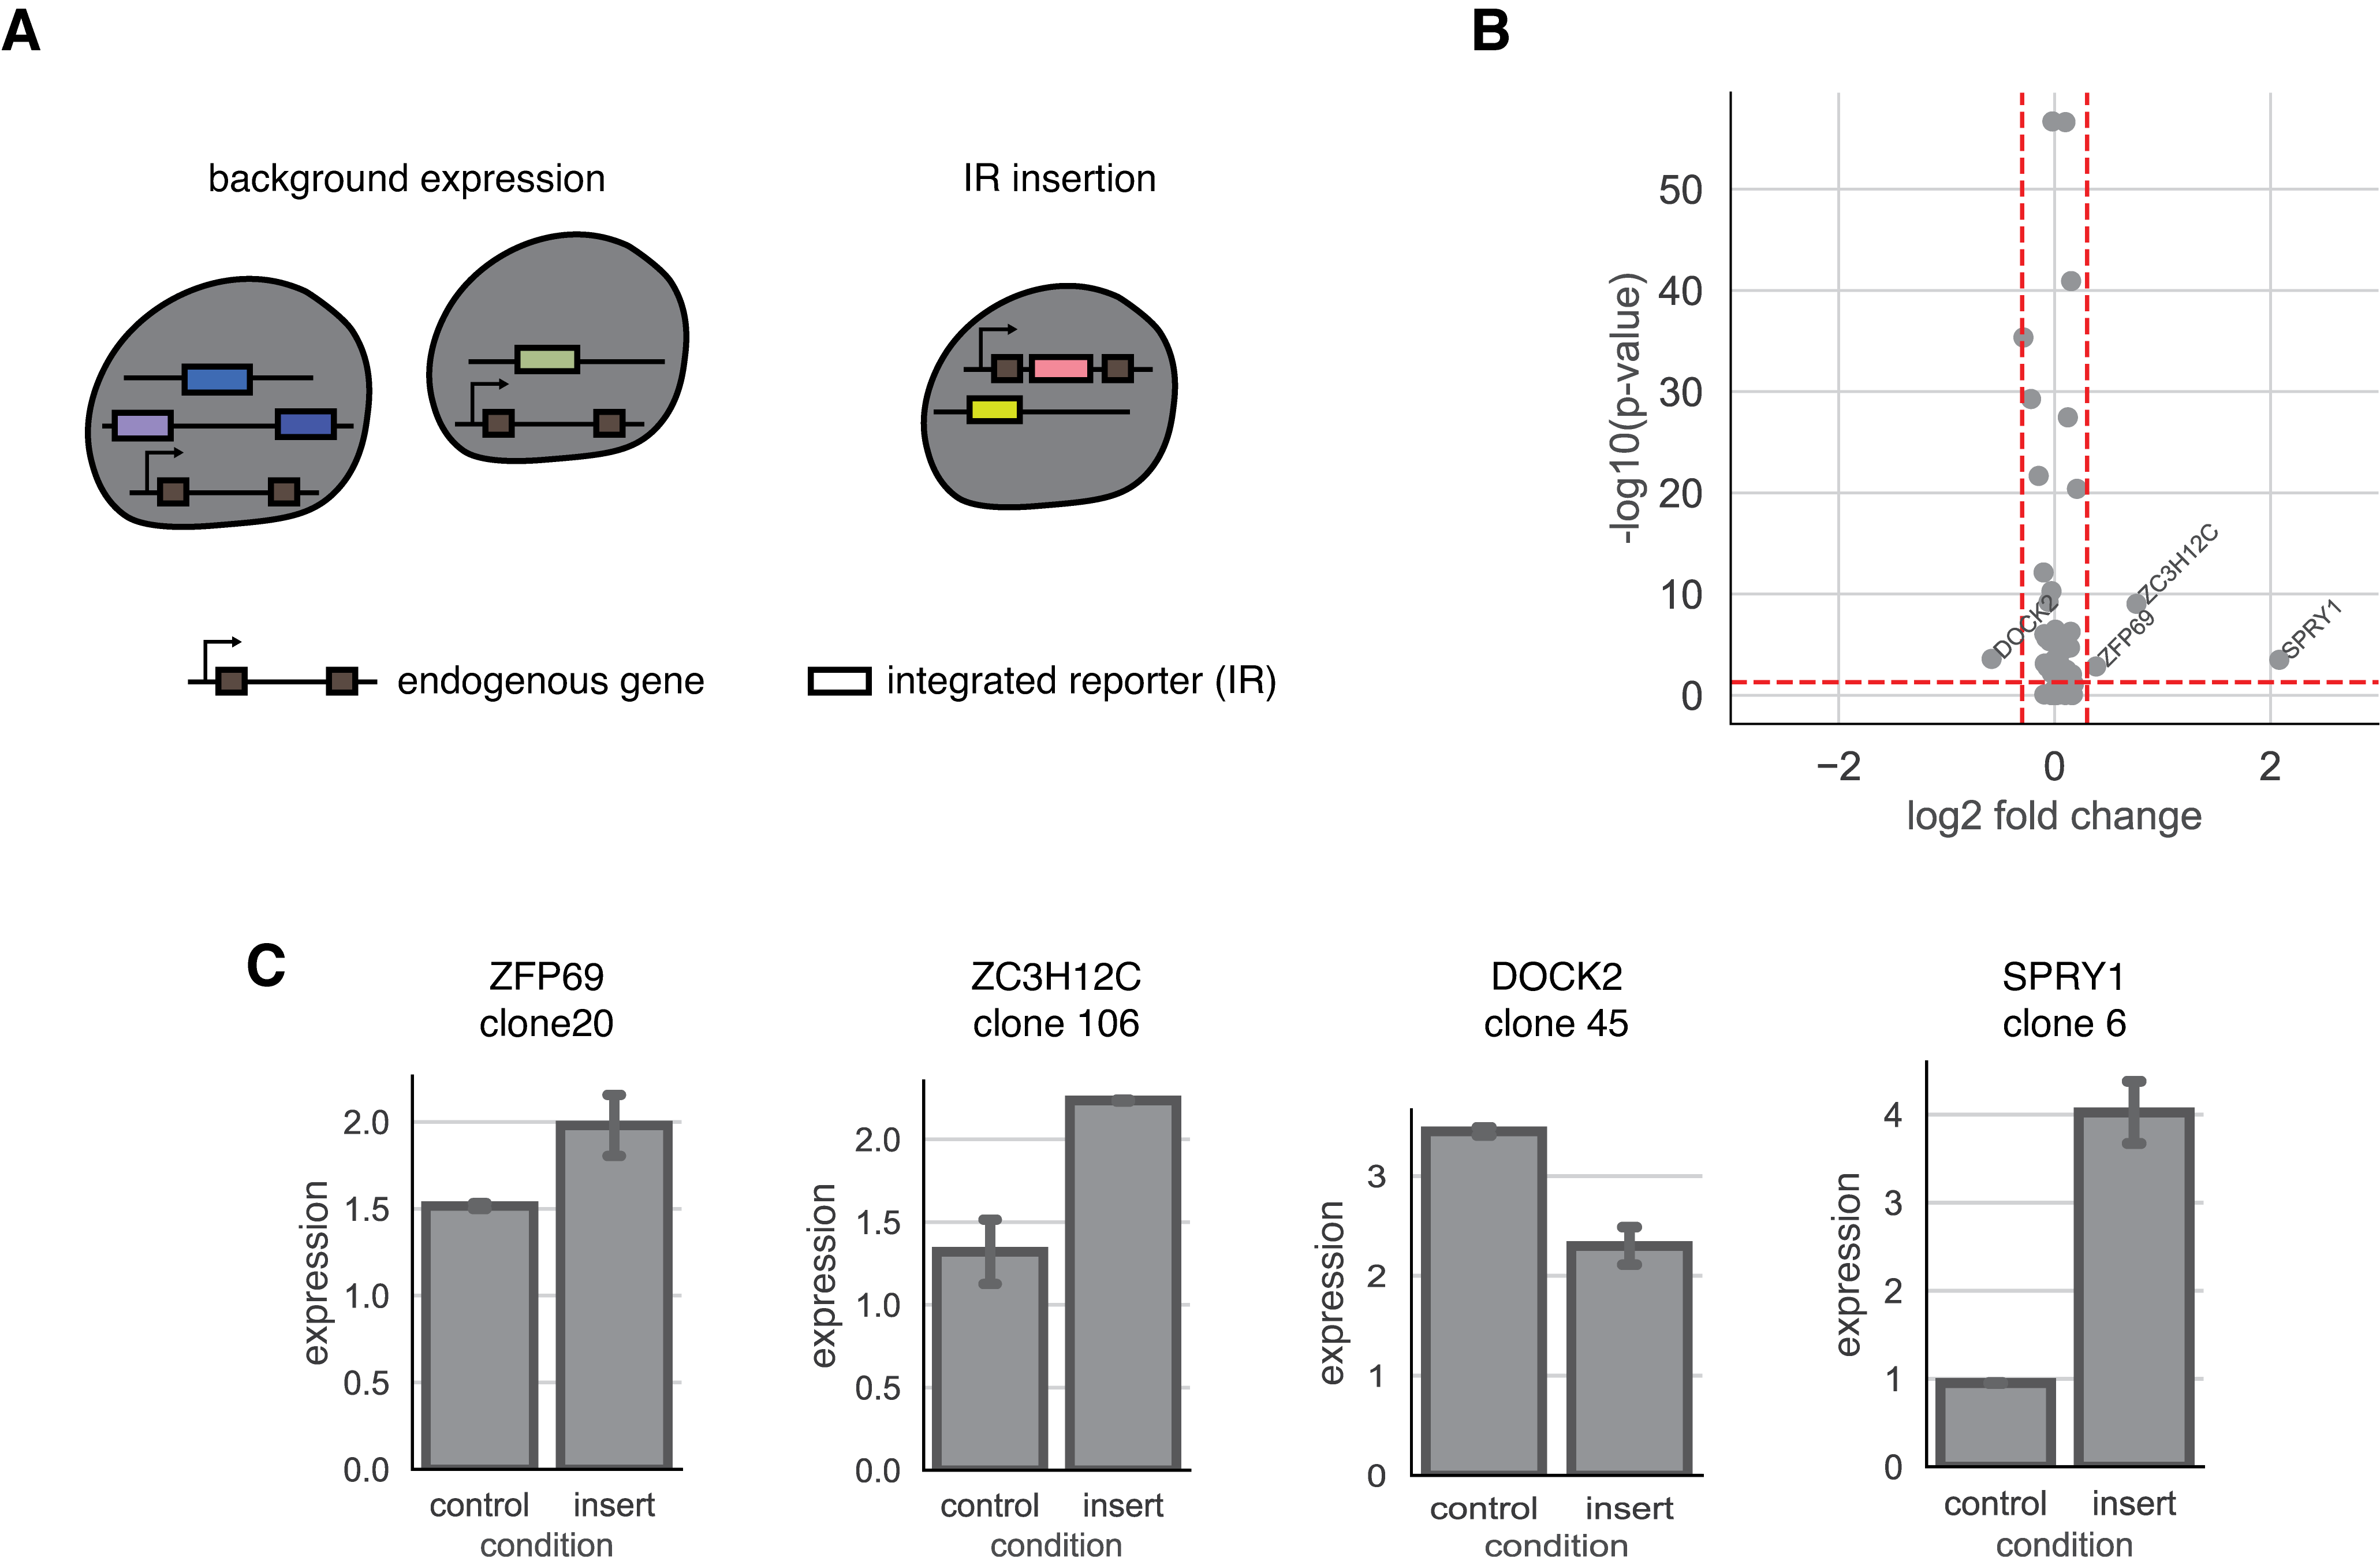
\includegraphics[width=\linewidth]{figures/cas_figure6.ai}
    \caption[SARGENT measures the insertion effect of a transgene.]{%
        \textbf{SARGENT measures the insertion effect of a transgene.}
        \subref{fig:cas_figure6a}
        Schematic for expression change detection in the transcriptome data.
        \subref{fig:cas_figure6b}
        Volcano plot of log\textsubscript{2} fold change and -log\textsubscript{10}(\textit{p}-value) from a Fisher’s Exact Test. Red dotted lines: cut off for fold change (0.5), cut off for \textit{p}-value (0.05).
        \subref{fig:cas_figure6c}
        Barplots of difference of expression between genes without IRs (control) and genes with IRs (insert). The clone where the IR is integrated is indicated. Error bars are derived from two technical replicates.
    }
    \label{fig:cas_figure6}
\end{figure}

\section{Discussion}

Since the early single-cell studies showing the variability of gene expression in isogenic populations \cite{elowitzmb_swainps:StochasticGene2002}, many individual chromatin and sequence features have been suggested to modulate expression noise \cite{raja_vanoudenaardena:NatureNurture2008, raja_tyagis:StochasticMRNA2006,bonnyar_el-samadh:OrthogonalControl2021, desairv_weinbergerls:DNARepair2021}. However, there has yet to be a systematic study of the impact of different genomic features on large numbers of identical genes. 
   
We developed SARGENT, a high throughput method to measure the expression mean and noise at different genomic locations in parallel. One key advantage of SARGENT is that the reporter gene used in all locations is identical, which allows us to isolate the effects of the genomic environments without being confounded by the effects of different promoters. We identified different chromatin marks that are associated with high or low MIN, and used a logistic regression model to identify features of the genomic environments that might control MIN. Our observations indicate that the features that control expression noise are independent of the features controlling expression mean. Several recent studies have developed tools for the orthogonal control of mean and gene expression noise \cite{bonnyar_el-samadh:OrthogonalControl2021,benzingerd_khammashm:PulsatileInputs2018, michaelsys_fulgata:PreciseTuning2019}. To this end, our results suggest potential mechanisms that can be targeted for independent modulation of expression mean and single-cell variability. 

We also quantified the extrinsic portion of expression noise and identified that the oscillation between a \enquote{stem-like} substate and a \enquote{differentiated} substate in K562 cells is an important source of extrinsic noise. Our data suggests that extrinsic noise might be more important in regulating MIN than genomic environments. This indicates that the regulation of noise of individual genes might be at the level of the promoter, rather than through its chromatin or genomic environment.
 
We envision that SARGENT will be a useful tool for other synthetic biology applications. While advances in genome engineering technologies now allow researchers to integrate transgenes at most desired genomic locations, the selection of appropriate sites for transgene overexpression remains non-trivial, with no location in human cells validated as a safe harbor locus \cite{papapetrouep_schambacha:GeneInsertion2016,pavanig_amendolam:TargetedGene2021}. This is mainly due to the lack of methods to systematically screen for loci that have high expression, low variability and do not impact cellular function. Here we showed that SARGENT can be used to read out a transgene’s impact on global expression as well as the endogenous gene that it is integrated into. Surprisingly, most endogenous genes are not impacted by the insertion of reporter genes. With SARGENT, we can quickly screen genomic locations to find the best locations for human transgene integration which will prove useful gene therapy applications.

More broadly, we envision that SARGENT will be a useful technology for many different applications including mechanistic studies of gene expression noise and synthetic biology applications. The 10x Genomics platform used in this study is limited by throughput, but improvements to scRNA-seq technologies will increase the scope of SARGENT. For example, coupling sci-RNA-seq \cite{caoj_shendurej:ComprehensiveSinglecell2017} or SPLiT-seq \cite{rosenbergab_seeligg:SinglecellProfiling2018} to SARGENT would allow for many more locations to be assayed in parallel. A larger goal will be to construct a detailed map of the MIN landscape across the genome, much like the maps of mean expression levels generated by ENCODE. 

\section{Methods}
\label{section:cas_methods}

\subsection*{SARGENT library cloning}

All primers and oligonucleotides used in this study are listed in \tref{tab:cas_tableS1}. To clone the reporter gene for SARGENT, we first cloned a CMV-BFP reporter gene containing the 10x capture sequence 1 (CS1) into a piggyBac vector containing two parts of a split-GFP reporter gene \cite{qiz_mitrard:OptimizedBroadly2017}. When the reporter gene construct is integrated into the genome, the split-GFP combines to produce functional GFP, allowing us to sort for cells that have successful reporter gene integrations. We next added a library of random barcodes to the plasmid by digesting the plasmid with XbaI followed by NEBuilder HiFi DNA Assembly (NEB \#E2621) with a single-stranded oligo containing 16 random N’s (Location barcodes; locBC) and homology arms to the plasmid (CAS P57). 

\subsection*{Generation of cell lines for SARGENT}

K562 cells were maintained in Iscove's Modified Dulbecco′s Medium (IMDM) + 10\% FBS + 1\% non-essential amino acids + 1\% penicillin/streptomycin. We selected two K562 cell lines previously used in our lab that each contain a \enquote{landing pad} at a unique location with a pair of asymmetric Lox sites for recombination (loc1 - chr8:144,796,786, loc2 - chr11: 16,237,204; hg38 coordinates). Using these \enquote{landing pad} cell lines allows us to perform smFISH on the landing pad to directly compare SARGENT and smFISH results. For each cell line, we replaced the original landing pad cassette with the same reporter gene in the SARGENT library so that we can capture the reporters from the landing pad and reporters from other genomic locations in SARGENT using the same primers. Pool 1 was derived from the loc2 cell line, while Pools 2, 3 and 4 were derived from the loc1 cell line.

The SARGENT library and piggyBac transposase were co-transfected into K562 (LP cell lines) cells at a 3:1 ratio using the Neon Transfection System (Life Technologies). For each experiment, we transfected 2.4 million cells with 9μg of SARGENT library and 3μg of transposase. The cells were sorted after 24 hours for GFP-positive cells to enrich for cells that have integrated SARGENT reporters. We reasoned that \textasciitilde100 single cells for each Integrated Reporter (IR) location would be required to obtain a good estimate of mean and variance. Each SARGENT experiment contains many single cell clone expansions: all the cells from the same clone share the same genomic integrations. Since we targeted approximately 20,000 cells per 10x run, the upper limit of the numbers of clones we can test in one experiment is 200. Because 10x also has a high dropout rate, we targeted 100 clones per experiment in order to ensure that we obtained high quality data. Each clone has an average of 5 integrations, which theoretically allows us to assay 500 IR locations in one experiment. Since the clones did not all grow at the same rate, practically we obtained fewer than 500 IRs per experiment.

For Pools 1 and 2, cells were sorted into pools of 100 cells each and allowed to grow until there were sufficient cells for RNA/DNA extraction and SARGENT experiments. Pool 3 contained the same cells as Pool 2, except that single cells were allowed to grow individually and pooled by hand just before the SARGENT experiments. This allowed for a more even representation of each individual clone (which contains unique integrations) in the final pool. For Pool 4, transfected cells were first sorted into 96-well plates with 2 cells/well and allowed to grow individually and 100 wells were manually pooled for SARGENT experiments. We used cells from Pool 4 to compute technical reproducibility.

\subsection*{SARGENT integration mapping}

We harvested DNA from SARGENT pools using the TRIzol reagent (Life Technologies). To map the locations of SARGENT integrations, we digested gDNA for each pool with a combination of AvrII, NheI, SpeI and XbaI for 16 hours. The digestions were purified and self-ligated at 16\dg C for another 16 hours. After purifying the ligations, we performed inverse PCR to amplify the barcodes with the associated genomic DNA region (CAS P59 and P64). For each pool, we performed 2 technical replicates with 8 PCRs per replicate and pooled the PCRs of each replicate for purification. We then used 8ng of each replicate for further amplification with 2 rounds of PCR to add Illumina sequencing adapters (CAS P55 and P65). The sequencing library was sequenced on the Illumina NextSeq platform. 

The barcodes of each read were matched with the sequence of its integration site. The integration site sequences were then aligned to hg38 using BWA with default parameters \cite{lih_durbinr:FastAccurate2009}. Only barcodes that mapped to a unique location were kept for downstream analyses. 

\subsection*{ClampFISH}
 
Single-molecule FISH was performed on the two \enquote{landing pad} locations that were in the original cell lines used for SARGENT (see Generation of cell lines for SARGENT above). ClampFISH probes for the reporter genes were designed using the Raj Lab Probe Design Tool. Each probe was broken into three arms to be synthesized by IDT. The 5’ of the left arm is labeled by a hexynyl group, and the 3’ of the right arm is labeled by NHS-azide. The right arm fragment was purified by HPLC. All three components were resuspended in nuclease-free H\textsubscript{2}O to a concentration of 400μM. The three arms were ligated by T7 ligase (NEB \# M0318), at 25\dg C overnight. then purified using the Monarch PCR \& DNA cleanup Kit (NEB \#T1030) and eluted with 40μl of nuclease-free water. After the ligation, each probe is stored at -20\dg C. ClampFISH was performed according to the suspension cell line protocol of clampFISH \cite{rouhanifardsh_raja:ClampFISHDetects2019}. 0.7 million cells were collected and fixed in 2mL of fixing buffer containing 4\% formaldehyde for 10 min, then permeabilized in 70\% EtOH at 4\dg C for 24 hours. The primary ClampFISH probes were then hybridized for 4 hours at 37\dg C in the hybridization buffer (10\% Dextran Sulfate, 10\% Formamide, 2X SSC, 0.25\% Triton X). After hybridization, cells were spun down gently at 1000 rcf for 2 min. Cells were washed twice with the washing buffer (20\% formamide, 2X SSC, 0.25\% Triton X) for 30 min at 37\dg C. The secondary probes were then hybridized to cells at 37\dg C for 2 hours and the cells were then washed twice with washing buffer for 30 min at 37\dg C. The primary and secondary probes are \enquote{clamped} in place through a click reaction (CuSO4 75μM, BTTAA 150μM, Sodium Ascorbate 2.5 mM in 2X SSC) for 20 min at 37\dg C. The cells were then washed twice in the washing buffer at 37\dg C for 30 min each wash. Then, the cells were hybridized with the hybridization buffer with tertiary probes for 2 hours at 37\dg C. We complete 6 cycles of hybridization for all our experiments. After the final washes, cells were incubated at 37\dg C with 100mM DAPI for 20 min, washed twice with PBS, resuspended in the anti-fade buffer, and spun onto a \#1.5 coverslip using a cytospin cytocentrifuge (Thermo Scientific), mounted onto a glass slide, sealed with a sealant, and stored at 4\dg C. 

\subsection*{SARGENT library using the 10x Genomics platform}

\subsection*{Cell preparation}

We used the Chromium Single Cell 3’ Kit (v3.1) from 10x Genomics for SARGENT. We followed the manufacturer’s instructions for preparing single-cell suspensions. We used a cell counter to measure the number of cells and viability, and used cell preparations with greater than 95\% cell viability. 

\subsection*{Cell barcoding and reverse transcription}

We followed the manufacturer’s instructions with the following modifications in Pools 1-3: no 10x template switching oligo (PN3000228) was added to the Master Mix (Step 1.1). To correct for the missing volume, 2.4μl of H2O was added to the master mix per reaction. For pool 4, the template switching oligo was included as written. For the cDNA amplification (Step 2.2), no 10x provided reagents were used. Instead, a custom primer (CAS P20) was used with 14 cycles of amplification with the provided 10x protocol (Step 2.2 d). For the pool where we also sequenced transcriptomes (Pool 4), we followed the 10x protocol as written for cDNA amplification. 

\subsection*{Barcode PCR and library preparation}

We performed nested PCRs to amplify barcodes from 10x cDNA. For pools 1-2, PCR library construction was split into two pools for amplification of transcripts captured by capture sequence 1 and poly(A) respectively. Both PCR reactions were done with 2μl purified cDNA, 2.5μl 10μM reporter-specific forward primer (CAS P45), 2.5μl 10 uM poly(A) (CAS P20) or capture sequence adapter-specific primers (CAS P32), and 25μl Q5 High Fidelity 2X Master Mix (NEB \#M0492) in 50μl total volume with 10 cycles amplification. The PCRs were then purified with Monarch PCR \& DNA Cleanup Kit (NEB \#T1030) and Illumina adapters were added in another 2 rounds of PCR, with a PCR purification step with the Monarch kit between PCRs. For poly(A) amplicons, we used CAS P42 and CAS PP2, followed by CAS P48 and CAS PP4. For capture sequence amplicons, we used CAS P41 and CAS CS2, followed by CAS P48 and CAS CS4. The reactions were then pooled and purified with SPRIselect Beads (Beckman Coulter) at 0.65x volume. For pool 4, we performed the PCRs for the poly(A) fraction using 2μl purified cDNA as described above, but not the capture sequence transcripts.

\subsection*{SARGENT data processing}
\subsection*{Read parsing}

We first identified the reads that match the constant sequence in our reporter gene. We used two versions of constant sequence to match against, depending on if the read was captured using the poly(A) sequence on the mRNA or the capture sequence specific to the 10x beads. We used a fuzzy match algorithm to capture reads that have a mismatch at these positions due to sequencing error. From each read, we parsed out the cell barcode, 10x UMI and locBC. We then collapsed reads with identical cell barcodes, UMI and locBCs into one \enquote{trio} and kept track of the number of reads supporting each trio. For downstream analysis, we filtered out trios with low numbers of supporting reads since these are likely to be enriched for PCR artifacts. We next processed the trios to error correct the cell barcodes and locBCs before estimating the mean and variance. 

\subsection*{Barcode error correction}

To correct for PCR artifact and sequencing errors, a custom script was used to error-correct for 10x cell barcodes. Briefly, we first acquired the empirical distribution of the Hamming distances among observed 10x cell barcodes. We found that more than 99\% of 10x cell barcodes are more than 6 hamming distances away from each other, making error correction a feasible approach to denoise the data. We first identify cell barcodes that match perfectly to the 10x cell barcode whitelist, then we order them based on their abundance. The cell barcodes that are not in the whitelist are then compared to the ordered whitelisted cell barcodes, if the Hamming distance between the non-whitelisted cell barcodes is within 2 Hamming distances of a whitelisted cell barcodes, we correct the unwhitelisted cell barcode. With cell barcode correction, we recovered \textasciitilde12\% of reads that would have been discarded. 

Due to the random synthesis of the locBC, a slightly different approach was taken for error correction for the locBCs. Briefly, all the locBCs are ranked based on abundance. Starting from the most abundant barcode, we look for locBCs that are within 4 Hamming distance to that barcode and correct them. We then remove that barcode and any corrected barcodes, and repeat this process until we have iterated through all locBCs.

\subsection*{Calculating mean and variance of each IR}

We filtered out cells that had less than 5 IR integrations (locBCs) and less than 10 UMIs. We also filtered out locBCs that were seen in less than 5 cells and UMIs that had less than 2 supporting reads. We then computed the number of UMIs per locBC in each cell to calculate the expression level of each locBC. For each locBC, mean expression was calculated as the average UMI count across all cells that expressed that locBC. Expression variance was calculated as the variance in UMI counts across all cells that expressed that locBC. 

\subsection*{Mean-independent noise (MIN) metric}

In order to remove the effect of the mean on the variance we first fit a linear model: $\log_2(\text{variance of IR location}) \sim \log_2(\text{mean of IR location})$ for each experiment al pool and used the residuals of the model as the mean-independent noise metric. For each IR location, the MIN is the residual variance after removing the effect of the mean.
Analyses of genomic environment effects on mean-independent noise

\subsection*{Chromatin environment association with mean/MIN}

We downloaded the Core 15-state chromHMM annotations for K562 cells from the Roadmap Epigenomics Project \cite{kundajea_kellism:IntegrativeAnalysis2015}. We then collapsed similar annotations and overlapped the IR locations with the corresponding annotation using the GenomicRanges R package \cite{lawrencem_careyvj:SoftwareComputing2013}. 

We split the IRs into locations with high vs low mean or high vs low MIN respectively. We then downloaded histone ChIP-seq datasets from ENCODE \cite{mooreje_wengz:ExpandedEncyclopaedias2020} and plotted the signals 10kb surrounding each class of IRs using the ComplexHeatmap package in R \cite{guz_schlesnerm:ComplexHeatmaps2016}. 

To look for enriched TF motifs we first downloaded all human motifs from the HOCOMOCO v11 database. We then filtered the motifs for TFs that are expressed (FPKM $\geq$ 1) in the K562 cell line using whole-cell long poly(A) RNA-seq data generated by ENCODE (downloaded from the EMBL-EBI Expression Atlas). We then used the STREME package \cite{baileytl_baileytl:STREMEAccurate2021} (MEME suite 5.4.1) with sequences of 1kb surrounding each IR to identify enriched de novo motifs in high or low MIN regions, using the other class as the control set of sequences. We then took the top 2 motifs for each bin and matched it against a list of TFs expressed in K562s using TOMTOM \cite{guptas_noblews:QuantifyingSimilarity2007} (MEME suite 5.4.1). We reported the top 6 TOMTOM matches. 

\subsection*{K562 Hi-C}

We performed Hi-C on wild-type K562 cells with the Arima Hi-C kit (A510008) according to the manufacturer's protocols (3 replicates, 870 million reads total). The reads were then processed with the Juicer pipeline \cite{durandnc_aidenel:JuicerProvides2016} to generate HiC contact files for each replicate. We then used the peakHiC tool \cite{bianchiv_laatw:DetailedRegulatory2019} to call loops from each IR with the following parameters: window size = 80, alphaFDR = 0.5, minimum distance = 10kb, qWr = 1. Using these parameters each IR was looped to a median of 3 regions (range 0-7). 

\subsection*{Logistic regression model for intrinsic and extrinsic features associated with MIN}

We used histone ChIP-seq and ATAC-seq datasets from ENCODE \cite{dunham2012n} and overlapped their signals with each IR using used bedtools v2.27.1 \cite{quinlanar_hallim:BEDToolsFlexible2010}. For all features we considered the 20kb upstream and downstream of each IR respectively. For each histone modification, we computed the mean ChIP signal around the IRs. For ATAC-seq, we calculated the total number of peaks with the bedtools map count option. To look for TF motifs we counted the numbers of each motif for TFs expressed in K562s (see above) in each surrounding IR sequence using FIMO \cite{grantce_noblews:FIMOScanning2011} (MEME suite 5.0.4). Because this resulted in a long list of TFs we further filtered the TFs to include only those with a significant correlation with MIN levels in the regression model. To determine the numbers of enhancers interacting with each IR we annotated the loops called from peakHiC above with chromHMM enhancer annotations using the GenomicInteractions R package \cite{harmstonn_lenhardb:GenomicInteractionsBioconductor2015} and counted the number of enhancers. 

For the extrinsic features, we calculated the proportion of cells in the \enquote{stem-like} substate and \enquote{differentiated} substate and different cell cycle phases based on the barcodes that appeared in those substates. We removed IR locations that have less than 30 cells in any of the substates.  

We used the glm function in R (version 3.6.3) to fit logistic regression models. We separated the IR locations into top 20\% MIN and bottom 20\% MIN and used logistic regression to classify locations. We first fit a model with just local sequence features (chromatin modifications, number of TF motifs, number of loops, whether the IR location is in a gene, GC content and the number of ATAC-seq peaks). We used data from one experiment for training the model and used data from another experiment as a holdout set of data to estimate the performance of the classifier. We next fit a model with cellular information for each IR location: proportion of cells with data for the IR location in S phase of the cell cycle, in G2 phase and the proportion of cells that are in the \enquote{stem-like} substate of K562 cells \cite{litzenburgerum_changhy:SinglecellEpigenomic2017}. Lastly, we fit a model that incorporated the extrinsic features and the significant predictors from the intrinsic features model.

\subsection*{Transcriptome analyses associated with SARGENT}

\subsection*{Processing the single-cell transcriptome data}

The single-cell RNAseq data was processed with CellRanger 6.0.1 and SCANPY 1.9.1 \cite{wolffa_theisfj:SCANPYLargescale2018}. Briefly, the raw reads were processed with the standard single-cell expression cell line pipeline line. The resulting expression matrix was then imported into SCANPY for further visualization and clustering. 

\subsection*{Identifying single cell clones}

We identified the individual clones for Pool 4 which contained cells that grew out of 100 two-cell clones. Since most of the clones will have unique integrations into unique genomic locations, the cells that grew out from the same clone will have identical unique sets of locBCs. Due to the dropout rates associated with scRNAseq methods, not all barcodes will be present in all cells, nor will the cell barcodes be uniquely linked to correct sets of locBCs. To identify the barcodes belonging to the same clone, we first recorded locBCs that are linked by a given cell barcode. We then filtered the locBC list associated with a given cellBC based on the number of UMIs associated with these locBC. At this step, we used a knee point detection algorithm \cite{satopaav_raghavanb:FindingKneedle2011} that automatically detects the inflection point of the ordered UMI counts histogram. After filtering for locBCs that appear in more than 5 cells, we constructed a clonal graph by linking locBCs that co-occur in the same cells.

\subsection*{Validation of individual clones}

We extracted gDNA from 16 clones that were grown out from Pool 4. We then amplified the barcodes from each clone using Q5 High Fidelity 2X Master Mix (NEB \#M0492) with primers specific to our reporter gene (CAS P58-59). For each clone, we performed 4 PCRs and pooled the PCRs for purification. 4ng from each clone was then further amplified with 2 rounds of PCR to add Illumina sequencing adapters (CAS P60-63). The barcodes were sequenced on the Illumina NextSeq platform. 

\subsection*{Estimating intrinsic vs extrinsic noise}

To understand how cellular environments affect IR expression, we computed the mean and standard deviation from all IR locations in the same cell. Since standard deviation is expected to increase with mean, we calculated the standard deviation/mean for each cell, which we termed the fluctuation index. To establish the null distributions, we randomly shuffled the cell labels for each clone and computed fluctuation indices for the shuffled cells. 

Intrinsic and extrinsic noise were estimated using the statistical framework developed for the dual-reporter experiment \cite{fuaq_pachterl:EstimatingIntrinsic2016}. In our experiment, single-cell expression differences among IR locations are treated as the intrinsic portion of the noise. We first extracted the pairwise expression level for IR locations in every single cell, then applied the above framework. The derivation is abbreviated and can be found in the original publication. Briefly, let C denote the expression for the first locBC in the cell, Y denote the expression for the second locBC in the cell and n denote the number of cells. 

Let $\eta_{\text {ext}}$ denote the extrinsic noise, and it can be calculated as:
$$
\eta_{\text {ext }}=\frac{1}{a \bar{C} \bar{Y}}\left(\sum_{i=1}^n C_i Y_i-n \bar{C} \bar{Y}\right)
$$
\centerline{where}
$$
% \begin{aligned} 
a=(n-1)\left(1+\frac{1}{n}\right)+\frac{1}{\rho^2} \\
$$
$$
\rho=\frac{\operatorname{Cov}[C, Y]}{\sqrt{\operatorname{Var}[C]} \sqrt{\operatorname{Var}[Y]}}
% \end{aligned}
$$
\\

Similarly, let $\eta_{\text {int}}$ denote the intrinsic noise, and it can be calculated as:
$$
% \begin{aligned}
\eta_{\text {int }}=\frac{1}{2 a \bar{C} \bar{Y}}\left(\sum_{i=1}^n\left(C_i-Y_i\right)^2-n(\bar{C}-\bar{Y})^2\right) 
% \end{aligned}
$$
\centerline{where}
$$
% \begin{aligned}
a=\frac{2 n^3-7 n+6}{2\left(n^2-n\right)}+\frac{2-n}{n^2-n} \frac{\rho}{1-\rho}+\frac{1}{2\left(n^2-n\right)}\left(\frac{\rho}{1-\rho}\right)^2 \\
$$
$$
\rho=\frac{\operatorname{Cov}[C, Y]}{\sqrt{\operatorname{Var}[C]} \sqrt{\operatorname{Var}[Y]}}
% \end{aligned}
$$

\subsection*{Cell substate impact on expression mean and noise}

To compute cell substate specific expression mean and noise at different genomic locations, individual cells were assigned a cell cycle phase of G1, S, or G2/M using a previously reported set of cell-cycle specific marker genes with SCANPY 1.9.1 \cite{wolffa_theisfj:SCANPYLargescale2018}. For the stem-like substate analysis, we clustered cells based on their transcriptomes and assigned cells in the CD24 high cluster as CD24+ cells \cite{litzenburgerum_changhy:SinglecellEpigenomic2017}. To ensure an accurate measurement of expression mean and noise, genomic locations with less than 15 cells in any phase were excluded from the cell cycle analysis. Based on this filtering criterion, 345 out of 939 genomic locations were used for this analysis. To determine the impact of cellular substates on gene expression noise, we calculated the proportion of cells in different cellular substates for each clone. For each clone, we also calculated the average mean and variance of all the IRs in that clone. 

\subsection*{Transgene integration analysis}

To examine whether the integration of a trans-gene alters endogenous gene expression, we first identified IR locations that were integrated into a gene body. Since the IR insertion only occurs in a single clone, we computed pseudobulk expression from cells in the clone using decouplerR 1.1.0 \cite{badia-i-mompelp_saez-rodriguezj:DecoupleREnsemble2022}. We then randomly sampled the same number of cells from all the other clones and used the pseudobulk expression from these cells as wild-type expression. To determine whether the expression in the IR clone is significantly different from wild-type expression, we computed the \textit{p}-value of differential expression using a Fisher’s exact test. 

\section{Supplementary Figures}

\beginsupplement

\begin{suppfigure}[htbp]  
    \centering
    \phantomlabel{fig:cas_figureS1a} 
    \phantomlabel{fig:cas_figureS1b}
    \phantomlabel{fig:cas_figureS1c}
    \phantomlabel{fig:cas_figureS1d}
    \includegraphics[width=\linewidth]{figures/cas_figureS1.ai}
    \caption[smFISH corroborates with SARGENT measurements.]{
        \textbf{smFISH corroborates with SARGENT measurements. (A,B)}
        Mean and noise levels of two IR locations (loc1 \subref{fig:cas_figureS1a} and loc2 \subref{fig:cas_figureS1b}) measured by SARGENT. Values were normalized (Z-scored) for comparison across different experiments.
        \textbf{(C,D)}
        Mean and noise levels of the same two IR locations (loc1 \subref{fig:cas_figureS1c} and loc2 \subref{fig:cas_figureS1d}) measured with smFISH. Error bars represent one std from two biological replicates. 
    }
    \label{fig:cas_figureS1}
\end{suppfigure}

\begin{suppfigure}[htbp]  
    \centering
    \phantomlabel{fig:cas_figureS2a} 
    \phantomlabel{fig:cas_figureS2b}
    \phantomlabel{fig:cas_figureS2c}
    \phantomlabel{fig:cas_figureS2d}
    \includegraphics[width=\linewidth]{figures/cas_figureS2.ai}
    \caption[Measurements of mean-independent noise across different chromosomal environments.]{
        \textbf{Measurements of mean-independent noise (MIN) across different chromosomal environments.}
        \subref{fig:cas_figureS2a}
        IR locations are distributed all throughout the genome. Each black bar above the ideogram represents a separate integration.
        \subref{fig:cas_figureS2b}
        IR locations are distributed across different chromatin types.
        \textbf{(C,D)}
        Expression mean is well correlated with fano factor \subref{fig:cas_figureS2c} and CV\textsuperscript{2} \subref{fig:cas_figureS2d}.  
    }
    \label{fig:cas_figureS2}
\end{suppfigure}

\begin{suppfigure}[htbp]  
    \centering
    \includegraphics[width=\linewidth]{figures/cas_figureS3.ai}
    \caption[Model results for high mean vs low mean.]{
        \textbf{Model results for high mean vs low mean.}
        Weights of features from the gene expression mean model using only intrinsic genomic features. Red bars: \textit{p}-value $<$ 0.05; Pink bars: 0.05 $\leq$ \textit{p}-value $<$ 0.1 from the logistic regression model.  
    }
    \label{fig:cas_figureS3}
\end{suppfigure}

\begin{suppfigure}[htbp]  
    \centering
    \phantomlabel{fig:cas_figureS4a} 
    \phantomlabel{fig:cas_figureS4b}
    \phantomlabel{fig:cas_figureS4c}
    \includegraphics[width=\linewidth]{figures/cas_figureS4.ai}
    \caption[Clonal identification allows for separation of intrinsic and extrinsic noise.]{
        \textbf{Clonal identification allows for separation of intrinsic and extrinsic noise.}
        \subref{fig:cas_figureS4a}
        Histogram of number of integrations per clone.
        \subref{fig:cas_figureS4b}
        Mock histogram showing the expected distributions if noise was either all intrinsic or all extrinsic.
        \subref{fig:cas_figureS4c}
        Histogram of measured fluctuation indices (defined as the standard deviation/mean of all IRs in a cell) for 10 random clones. The shuffled distribution represents the distribution after cell labels have been shuffled, which simulates the case when all noise is intrinsic.   
    }
    \label{fig:cas_figureS4}
\end{suppfigure}

\begin{suppfigure}[htbp]  
    \centering
    \phantomlabel{fig:cas_figureS5a} 
    \phantomlabel{fig:cas_figureS5b}
    \phantomlabel{fig:cas_figureS5c}
    \phantomlabel{fig:cas_figureS5d}
    \phantomlabel{fig:cas_figureS5e}
    \phantomlabel{fig:cas_figureS5f}
    \includegraphics[width=\linewidth]{figures/cas_figureS5.ai}
    \caption[Cell cycle and CD24 states partially explain extrinsic noise.]{
        \textbf{Cell cycle and CD24 states partially explain extrinsic noise.}
        \subref{fig:cas_figureS5a}
        UMAP clustering reveals CD24+ cell population.
        \subref{fig:cas_figureS5b}
        CD24+ cells express stemness and proliferation marker gene GATA1.
        \textbf{(C,D)}
        Violin plots of MIN \subref{fig:cas_figureS5c} and mean \subref{fig:cas_figureS5d} levels in different phases of the cell cycle. \textit{P}-values were calculated using the Mann-Whitney-Wilcoxon test. Legend: $\ast$: 0.01 $<$ \textit{p}-value $\leq$ 0.05, $\ast\ast$: 0.001 $<$ \textit{p}-value $\leq$ 0.01, $\ast\ast\ast$: 0.0001 $<$ \textit{p}-value $\leq$ 0.001, $\ast\ast\ast\ast$: \textit{p}-value $\leq$ 0.0001. ns: not significant.
        \subref{fig:cas_figureS5e}
        Gene expression mean model improves after the addition of extrinsic features.
        \subref{fig:cas_figureS5f}
        Weights of features from the mean model using both intrinsic genomic and extrinsic features. Red bars: \textit{p}-value $<$ 0.05; Pink bars: 0.05 $\leq$ \textit{p}-value $<$ 0.1 from the logistic regression model. 
    }
    \label{fig:cas_figureS5}
\end{suppfigure}

\begin{suppfigure}[htbp]  
    \centering
    \phantomlabel{fig:cas_figureS6a} 
    \phantomlabel{fig:cas_figureS6b}
    \includegraphics[width=\linewidth]{figures/cas_figureS6.ai}
    \caption[IR integrations have little impact on endogenous expression.]{
        \textbf{IR integrations have little impact on endogenous expression.}
        \subref{fig:cas_figureS4a}
        Bar plot number of IRs in endogenous genes per clone.
        \subref{fig:cas_figureS4b}
        Shuffling IR-endogenous gene labels results in no differentially expressed genes.   
    }
    \label{fig:cas_figureS6}
\end{suppfigure}

\clearpage

\section{Supplementary Tables}

\begin{supptable}[htb]
    \centering
    \caption{Primers used in this study}
      \begin{tabular}{lp{13cm}}
      \toprule
      \textbf{Name} & \textbf{Sequence} \\
      \midrule
      CAS P20 & CTACACGACGCTCTTCCGATCT \\
      CAS P32 & GTCAGATGTGTATAAGAGACAG \\
      CAS P41 & GTGACTGGAGTTCAGACGTGTGCTCTTCCGATCTTCTCGCTTCGAGTCTAGA \\
      CAS P42 & GTGACTGGAGTTCAGACGTGTGCTCTTCCGATCTAGCTCTCGCTTCGAGTCTAGA \\
      CAS P45 & TCTCGCTTCGAGTCTAGA \\
      CAS P48 & CAAGCAGAAGACGGCATACGAGATNNNNNNNNNGTGACTGGAGTTCAGAC \\
      CAS P55 & GTGACTGGAGTTCAGACGTGTGCTCTTCCGATCTTAGGACCGGCCTTAAAGC \\
      CAS P57 & GGGGCACAAGCTTAATTGAGAGCTCTCGCTTCGAGTCTAGANNNNNNNNNNNNNNNNCTCGAGTTGTGGCCGGCCCTT \\
      CAS P58 & TGCCTGGCGTCTACTATGTG \\
      CAS P59 & AACGCCAGGGTTTTCCCAA \\
      CAS P60 & CTTTCCCTACACGACGCTCTTCCGATCT(N[1-4])CTCGCTTCGAGTCTAGA \\
      CAS P61 & GTGACTGGAGTTCAGACGTGTGCTCTTCCGATCTGCCAGGGTTTTCCCAAC \\
      CAS P62 & AATGATACGGCGACCACCGAGATCTACACNNNNNNACACTCTTTCCCTACACGACGCT \\
      CAS P63 & CAAGCAGAAGACGGCATACGAGATNNNNNNNNNGTGACTGGAGTTCAGACGTG \\
      CAS P64 & GTACGCATGCCGCATGATTATCTTTAACGTACGTCAC \\
      CAS P65 & ACGACGCTCTTCCGATCTGCTCGA(N[1-4])GTACGTCACAATATGATTATCTTTCTAG \\
      CAS PP2 & ATCTACACTCTTTCCCTACACGACGCTCTTC \\
      CAS PP4 & AATGATACGGCGACCACCGAGATCTACACTCTTTCCCTACA \\
      CAS CS2 & CGAGATCTACACTCGTCGGCAGCGTCAGATGTGTATAAGAGACAG \\
      CAS CS4 & AATGATACGGCGACCACCGAGATCTACACTCGTCG \\
      \bottomrule
      \end{tabular}%
    \label{tab:cas_tableS1}%
  \end{supptable}%
  

\chapter{Discussion}
\label{chap:conclusion}
\tightlists

Recent years have shown that there is a lot of cell-to-cell variability in gene expression. However what does this variability mean? How does a cell respond to signals that are so variable between cells? How are biological processes regulated with high fidelity in the face of such variability. A lot of work has been carried out to answer these questions over the years. My thesis work provides a few more hints about how such systems operate.

In the second chapter of this thesis I looked at variability amongst cells responding to the hedgehog signaling pathway. I found that overexpression of a single transcription factor was able to make more cells respond faster. The cell-to-cell variability in gene expression of this single transcription factor could underlie important developmental decisions. It thus becomes important to understand what underlies the cell-to-cell variability in gene expressionof different genes.

In the second chapter of my thesis I helped develop a new technology to measure the cell-to-cell variability of the same reporter gene inserted in multiple genomic locations. By looking at how the cell-to-cell variability changes with the features of the different genomic locations I was able to understand what are the features that determine high cell-to-cell variability and low cell-to-cell variability. I also found that most of the cell-to-cell variability was determined by the mean level of expression, and removing the effect of the mean leaves a very small amount of variability that we studied.

In this chapter, I will dicuss the implications of these two pieces of work. Specifically, I will first touch on how I think the cell makes decisions in the face of so much cell-to-cell variability. Next, I will discuss whether we should study cell-to-cell variability in gene expression especially when most of the variability can be explained by the mean expression level. Finally, I will touch upon how this work can be expanded upon in the future.

\section{How are cellular decisions made in the face of noise?}

In the first project I showed that the cell-to-cell variability of a single transcription factor Prrx1 can influence whether a cell responds to a perturbation or not. One model that might explain how the cell responds is by using a threshold model for any cellular decision. The threshold model suggests that cells that have a level of protein above a certain level are the ones that are poised to respond. Cells that are below a protein level are the ones that don't respond. When a population of cells are induced to express a certain gene, the mean level of expression increases but often the mean level increase is accompanied by an increase in the cell-to-cell variability. However, the proportion of cells that respond to a stimuli is determined by the proportion of cells that are able to express the gene above a certain level. This model fits with what I observe in Prrx1.

In the model for hedgehog signaling in \label{Chap:hedgehog} we hypothesized that stochastic activity of transcription factors might underlie why some cells are able to respond faster to hedgehog perturbation vs others. We identified a lost of candidate transcription factors that are overexpressed in the fast responding cells and tested five TFs. We found that overexpressing one of the transcription factors Prrx1 is able to increase the proportion of cells that respond faster. In a threshold model of cellular decision making, cells that have sufficient activity of Prrx1, above a certain threshold, are able to respond to the hedgehog stimulation.  When we induce Prrx1 expression, we increase the mean and variance of Prrx1. However the proportion of cells that express Prrx1 above a certain threshold are able to respond. A follow-up question from this study is how many such regulators exist and how might we find them?

We identified the fast responder gene signature consisting of 300 candidates. In theory, there might be some false positives amongst this list of 300 genes. However, in our model a TF that is able to express a sufficient fraction of these 300 genes is able to make the cells respond. When we overexpress Prrx1, we showed that we misexpress 74 of the 300 genes. Could the 74 genes be the ones that matter? I think this question still remains to be answered. It could be that only a small fraction of the 74 genes matters. Or it could be the case that Prrx1 operates through a different mechanism where it turns on Gli2, and that's all that matters for the hedgehog signaling. We tried approaches looking for motifs in the 300 genes, and identifying enriched TFs in the promoter regions of the 300 genes, however we were limited by the number of TFs that we could test for their effect on the hedgehog response. 




My thesis consists of two main parts. 
In the first part I investigated cell-to-cell variability in the hedgehog pathway... We showed
In the second chapter we integrated the same reporter gene and looked at how the cell to cell variability changes across 
different integrations across the genome. .. We did.. we showed.. 

no stochastic activation of hedgehog pathway in 3T3 cells

Prrx1 can induce a faster response. how does it do it. how many other regulators are there.

\subsection{what do these results mean}


\subsection{what can we do by controlling noise}
- gene therapy

\subsection{Future Directions}
In this section I will describe future directions of the two projects that I worked on. I hope this section will provide somewhat useful to anyone studying cell-to-cell variability or graduate students in general.

In the second chapter, I was able to show how hedgehog signaling was faster in cells when I overexpressed a single transcription factor Prrx1. However, it remains unknown how many other transcription factors are able to do this. And is there a way to predict the genes that reduce this variability from the 300 candidates that we have computationally instead of testing them out one by one experimentally. We used approaches like cell-oracle \cite{cell-oracle} to predict which TF perturbation might change the cell state from the slow-responder to fast-respodner cell state. These approaches which integrate multiple lines of evidence including cell-state differential expression, transcription factor binding data, and chromatin accessibility data to predict the effects of TF perturbations. However, such approaches are still in their infancy and there is a lot of work that can be done here to develop computational approaches to predict perturbation effects. Data such as what I have generated for this thesis work - RNA-seq data after overexpressing multiple transcription factors either through plasmid transfection or in stably integrated cell-lines can be used to train such computational models. If these models are accurate enough, this would could potentially minimize the number of functional experiments and provide a list of high confidence genes to test.

On the technology side of things, in the second and third chapters we  used single-cell RNA sequencing to look at the cell-to-cell variability of different genes. Single-cell RNA sequencing, as discussed in Chapter 1, in-theory helps to measure the expression of all polyA transcripts within a cell. However, the current methods of transript capture are still far from perfect. Only a small fraction of the overall transcripts within a cell are captured \cite{pachter's postdoc} and it is unclear how random this dropout is amongst transcripts. I am optimistic that these technical challenges will be mostly solved over the next decade, this would further increase the statistical power of the approaches used in this thesis to detect true effects. The fold-changes that we detect in the expression of transcription factors between the slow responders and fast-responders is pretty small. More precise measurements of transcripts could potentially result in a smaller and more high-confidence set of candidate genes that are differentially expressed between sub-states. In Chapter 3, the mean independent noise is a small fraction of the overall noise levels of a gene. Having more precise measurements of noise will also improve our ability to Approaches such as merfish \cite{merfish} which use imaging to measure multiple transcripts within a cell could provide an alternative avenue to sequencing. However imaging approaches are currently very challenging to setup, and harder to scale compared to sequencing. This may very well change in the future.

We've used a computational method for tracking the trajectory that cells take during a cellular process, i.e hedgehog signaling. This approach is far from perfect, and in the future I expect there may be better technologies to trace the series of cell-state changes that a cell undergoes when confronted with a perturbation. Already barcode-based approaches are available \cite{morris lineaage tracing, arnav's paper}, however even these approaches are not fool proof and are largely expensive due to dropout issues. The availability of better lineage tracing technologies will further the study of cell-to-cell variability and shed light on why approaches like reprogramming are inefficient.

In chapter 2, we've integrated the same reporter gene in multiple locations to understand what features are associated with cell-to-cell variability. In the future, ony might imagine integrating different reporter genes or the same gene with different cis-regulatory elements genome-wide and study cell-to-cell variability in a similar approach. Indeed similar approaches have been used to study the impact of genomic location on mean expression \cite{claraice's papers}, however precise single-cell measurements will extend this to studying cell-to-cell variability. This approach would be invaluable for gene-therapy approaches, if there are interactions between a gene and it's local environment, and enable choosing locations with low variability. The same cis-regulatory element might have the same mean at different locations but different cell-to-cell variability, current bulk approaches that study just the mean level of expression are blind to such interesting phenomena.


hedgehog:
molecular barcoding instead of trajectory analysis
increase accessible cholesterol instead of srebf2
How can we identify other TFs that drive noise?



cas:
scaling up to more number of cells using scirnaseq




\begin{SingleSpace}
\printbibliography
\end{SingleSpace}

\appendix

\end{document}
